\documentclass[11pt, a4paper]{article}

% Codificación e idioma
\usepackage[T1]{fontenc}
\usepackage[utf8]{inputenc}
\usepackage[spanish,es-noshorthands]{babel}
\usepackage{csquotes}

% Bibliografía
\usepackage[backend=biber, style=apa]{biblatex}
\addbibresource{referencias.bib}

% Matemáticas
\usepackage{amsmath}
\usepackage{amssymb}

% Tablas y figuras
\usepackage{booktabs}
\usepackage{array}
\usepackage{multirow}
\usepackage{graphicx}
\usepackage{float}
\usepackage{caption}
\usepackage{subcaption}
\usepackage{placeins}

% Listas
\usepackage{enumitem}

% Formato de página
\usepackage[margin=2.5cm]{geometry}

% Enlaces
\usepackage[colorlinks=true, linkcolor=blue, urlcolor=blue, citecolor=blue]{hyperref}

% Diagramas
\usepackage{tikz}
\usetikzlibrary{shapes.geometric, arrows.meta, positioning, fit, backgrounds}
\usepackage{xcolor}
\definecolor{sup}{HTML}{4CAF50}
\definecolor{vlmgen}{HTML}{C62828}
\definecolor{vlcls}{HTML}{1565C0}

\graphicspath{{imagenes/}}

\title{\textbf{Experimentación: Clasificación y Generación de Reportes\\ de Lesiones de Piel con Modelos Visión--Lenguaje}}
\author{Facundo Tomás Gaviola}
\date{\today}

\begin{document}
\maketitle

\noindent\fbox{\begin{minipage}{\dimexpr\textwidth-2\fboxsep-2\fboxrule\relax}
\small
\textbf{Nota de actualización (octubre de 2026).} Las cifras del cuerpo de este documento se obtuvieron
con una partición de HAM10000 \emph{por imagen}, que dejaba el 36\% del test con lesiones vistas en
entrenamiento (fuga de información), y con el ganador del barrido elegido por F1 ponderado. La
experimentación se rehízo con una partición \emph{disjunta por lesión}, el ganador elegido por F1 macro
en validación y tres semillas; la cascada se regeneró con el clasificador nuevo. El cuerpo no se reescribió:
las cifras vigentes, que son las de la tesina, son las de esta tabla.

\smallskip
\centering
\footnotesize
\begin{tabular}{@{}p{0.42\textwidth}ll@{}}
\toprule
\textbf{Resultado} & \textbf{En este documento} & \textbf{Vigente} \\
\midrule
Swin-Tiny: exactitud / F1 macro / sens.\ macro & 0.868 / --- / 0.870 & 0.846 / 0.733 / 0.692 ($\pm$0.025) \\
ConvNeXt-Tiny: exactitud / sens.\ macro & 0.827 / 0.849 & 0.843 / 0.691 \\
Ensamble Swin$+$ConvNeXt: exactitud / sens.\ macro & --- & 0.855 / 0.706 \\
DenseNet121 / ViT-B/16: exactitud (receta de su familia, 3 semillas) & 0.846 / 0.858 & 0.822 / 0.836 \\
Pesos por clase (Swin): sens.\ macro con CE simple $\to$ con pesos & sin ganancia & 0.707 $\to$ 0.783 \\
ECE de Swin-Tiny (sin calibrar) & 0.380 (subconfiado) & 0.040 (sin pesos por clase) \\
Melanoma, Swin: AUC / sens.\ con esp.\ $\geq$0.85 & 0.931 / 0.862 & 0.921 / 0.796 \\
Melanoma, ensamble: AUC / sens.\ con esp.\ $\geq$0.85 & --- & 0.926 / 0.828 \\
DermLIP zero-shot: exactitud / sens.\ macro$^{\dagger}$ & 0.377 / 0.510 & 0.716 / 0.544 \\
DermLIP SVM vs Swin-ImageNet congelado: sens.\ macro & 0.788 vs 0.579 & 0.673 vs 0.466 \\
HIBA, Swin: exactitud / sens.\ macro & 0.585 / 0.532 & 0.546 / 0.424 \\
Ruteo de 3 niveles: cobertura de lo presentado & 0.934 & 0.904 \\
Cascada, consistencia con Swin$^{\ast}$: Mini-VLM / LLaVA-Med / SkinVL & 0.812 / 0.696 / 0.80 & 0.849 / 0.745 / 0.846 \\
Pipeline avanzado$^{\ast}$, Mini-VLM: simple $\to$ avanzado & 0.82 $\to$ 0.94 ($+$0.118) & 0.858 $\to$ 0.901 ($+$0.043) \\
Pipeline avanzado$^{\ast}$, LLaVA-Med: simple $\to$ avanzado & 0.706 $\to$ 0.831 ($+$0.125) & 0.755 $\to$ 0.744 ($-$0.011, n.\,s.) \\
\bottomrule
\end{tabular}

\smallskip
\raggedright
Cambios de interpretación: (1) las pérdidas para desbalance sí suben la sensibilidad macro, a costa de
exactitud y F1 macro; (2) la subconfianza de la calibración venía de los pesos por clase y de ajustar la
temperatura sobre un val solapado con train; (3) la ganancia del pipeline avanzado es menor porque el
clasificador nuevo deja menos casos inciertos (248 en vez de 334); (4) con la métrica oficial, el
pipeline avanzado no mejora el reporte de LLaVA-Med: su ganancia anterior venía de razonamiento
\texttt{<think>} sin cerrar que nombraba los candidatos. $^{\ast}$Métrica oficial: consistencia solo sobre el
reporte (sin \texttt{<think>}, también el que queda abierto), con \emph{matcher} estricto
(\texttt{ensemble\_bootstrap*\_les\_report\_only\_strict.json}, actualizado el 18/10/2026). Las conclusiones
centrales se sostienen. \texttt{full\_uncertainty} y la taxonomía por clase quedan con el anclaje anterior; RAG se
regeneró con el índice por lesión (11/10/2026, Sección~\ref{sec:rag}). $^{\dagger}$Protocolo oficial de Derm1M (ocho plantillas y nombres de clase de los autores, p.\,ej.\ ``nevus''); con ``melanocytic nevus'' los nevos se clasificaban como MEL (24/10/2026, \texttt{resul/dermlip\_zs\_protocolo\_resul\_20261024.md}). La condición de la cascada con diagnóstico de DermLIP (``0.38'') usa las predicciones anteriores.
\end{minipage}}
\bigskip

\begin{abstract}
\noindent
Este documento reporta de forma detallada los experimentos realizados para la tesina, organizados en
torno a dos preguntas centrales: \textbf{(1)} ¿pueden los Modelos Visión--Lenguaje (\emph{Vision--Language
Models}, VLMs) clasificar lesiones de piel con una precisión comparable a la de los clasificadores
visuales tradicionales?, y \textbf{(2)} ¿pueden generar reportes clínicos confiables a partir de la
imagen? El trabajo se desarrolló de manera \emph{iterativa}: cada resultado es analizado y medido, y a
partir de ese análisis se decide cuál es el siguiente experimento. Hasta el momento, la evidencia
sugiere que, en clasificación, los VLMs médicos generales no resultan competitivos frente a los modelos
especializados, y que el factor determinante no parece ser la modalidad ``VLM'' sino la
\emph{especialización de dominio}; en generación, los VLMs producen descripciones ricas pero
diagnósticamente poco confiables, una limitación que un sistema en cascada (clasificador + generador con
\emph{grounding}) mitiga de forma sustancial, y que un \textbf{ensamble consciente de la incertidumbre}
—que además de afirmar cuando hay confianza, ofrece un diferencial o deriva a un especialista cuando no la
hay— mejora todavía más: la fidelidad diagnóstica (\emph{diagnostic consistency}) sube de $0.82$
(\emph{grounding} simple) a $0.94$ sobre los casos no derivados, validado \emph{end-to-end} sobre los
reportes generados. El alcance de estas conclusiones está acotado: se sostienen sobre dermatoscopía de una
población concreta —con una caída documentada al transferir a otra— y sobre métricas automáticas, ya que
la validación por un especialista, cuyo instrumento queda preparado, excede el alcance de esta
experimentación.
\end{abstract}

\tableofcontents
\bigskip

% ============================================================
\section{Introducción}
\label{sec:intro}
% ============================================================
El diagnóstico asistido de lesiones de piel combina dos tareas complementarias: \emph{clasificar} la
lesión (asignarle una categoría diagnóstica) y \emph{describirla} mediante un reporte clínico. Los VLMs
—que acoplan un codificador visual a un modelo de lenguaje— prometen abordar ambas con un solo sistema.
Es por esto que se pone a prueba esa promesa de manera empírica, y este documento detalla el recorrido
experimental, los resultados obtenidos y las conclusiones (parciales) que se desprenden.

\paragraph{Un proceso iterativo.} La experimentación se realizó en un ciclo de
\emph{hipótesis $\rightarrow$ ejecución $\rightarrow$ análisis $\rightarrow$ decisión}: cada resultado
se midió con métricas definidas de antemano y, según ese análisis, se decidió el siguiente experimento.
Este enfoque fue necesario porque varios resultados contradijeron las hipótesis iniciales y obligaron a
re-diagnosticar el problema. El recorrido, que las secciones siguientes desarrollan en detalle, fue:

\begin{enumerate}[leftmargin=1.6em]
  \item \textbf{Baseline de clasificación.} Se entrenaron clasificadores supervisados (redes
  convolucionales y \emph{Vision Transformers}) sobre HAM10000, para tener un punto de comparación
  fuerte (Sección~\ref{sec:clasif}).
  \item \textbf{VLMs en clasificación.} Se evaluaron VLMs médicos generales con cuatro estrategias:
  (i) \emph{zero-shot}, pidiéndole al modelo la clase y leyendo su respuesta; (ii) \emph{likelihood
  scoring}, eligiendo la clase a la que el modelo asigna mayor probabilidad; (iii) razonamiento
  estructurado (\emph{Chain-of-Thought}); y (iv) \emph{fine-tuning} (ajuste fino). Estas estrategias se
  explican en detalle en la Sección~\ref{sec:clasif_diseno}. Los resultados fueron muy inferiores al
  baseline.
  \item \textbf{Primera hipótesis y su refutación.} Se conjeturó que la causa era el \emph{desbalance}
  de clases. Para verificarlo se realizó una iteración de re-entrenamiento orientada a re-balancear y,
  además, se inspeccionaron los datos y las predicciones. La hipótesis no se sostuvo: el bajo
  rendimiento aparece incluso \emph{sin} entrenamiento (en \emph{zero-shot}), los datos de entrenamiento
  no están sesgados hacia las clases problemáticas, y el modelo concentra sus predicciones en clases
  distintas según la configuración. La Sección~\ref{sec:rediag} presenta esta evidencia.
  \item \textbf{Especialización de dominio.} Guiados por el estado del arte, se incorporó un modelo
  visión--lenguaje \emph{específico de dermatología} (DermLIP). Este \emph{recuperó la capacidad de
  discriminar} entre clases —que los VLMs generales habían perdido— acercándose al desempeño de los
  clasificadores supervisados, aunque sin superarlos en exactitud absoluta (Sección~\ref{sec:dermlip}).
  \item \textbf{Generación de reportes y \emph{la contribución metodológica central}.} Se ajustaron los
  VLMs para generar reportes. El análisis reveló un problema de fidelidad diagnóstica y un sesgo en la
  forma de evaluar; a partir de ese diagnóstico se diseñó e iteró un \textbf{ensamble en cascada}
  (clasificador especializado $\rightarrow$ generador con \emph{grounding} —se le \emph{ancla} al VLM el
  diagnóstico del clasificador antes de redactar, en vez de dejarlo generar a ciegas; se define en detalle
  en la Sección~\ref{sec:gen}) que mejoró sustancialmente los
  resultados y constituye la propuesta metodológica del trabajo (Sección~\ref{sec:gen}).
  \item \textbf{Análisis de rigor, robustez y costo.} Alrededor de estos ejes se realizaron análisis
  complementarios —calibración de las probabilidades, significancia estadística, robustez a cambio de
  población (OOD) y de calidad de imagen, interpretabilidad, taxonomía de errores, ablaciones del ensamble
  y costo computacional— que profundizan y ponen a prueba las conclusiones anteriores.
\end{enumerate}

Un eje transversal atraviesa todo el recorrido: el de \textbf{hardware accesible}. Los clasificadores
supervisados usados (Swin-Tiny, ConvNeXt-Tiny, $\sim$28\,M de parámetros) y los VLMs ajustados con LoRA
corren en GPUs de consumo (RTX 4070/4080, $12$--$16$\,GB), no en infraestructura de cómputo dedicada; se
prioriza deliberadamente esta franja de costo por sobre perseguir el máximo desempeño absoluto con modelos
de mayor escala. Este criterio reaparece en la evaluación de melanoma
(Sección~\ref{sec:melanoma}) y se retoma explícitamente en el análisis de costo
(Sección~\ref{sec:costo}) y en la síntesis final.


% ============================================================
\section{Configuración experimental}
\label{sec:config}
% ============================================================
\subsection{Conjuntos de datos}
\label{sec:datasets}
Se utilizaron cinco conjuntos de datos, con roles diferenciados (Cuadro~\ref{tab:datasets}). Es
importante notar que \emph{no todos se usaron para lo mismo}: algunos para entrenar, otros solo para
evaluar, y difieren en la modalidad de imagen.

\begin{table}[H]
  \centering
  \caption{Conjuntos de datos y su rol en la experimentación.}
  \label{tab:datasets}
  \small
  \begin{tabular}{p{2.8cm}p{3cm}p{2.4cm}p{6.1cm}}
    \toprule
    \textbf{Dataset} & \textbf{Modalidad} & \textbf{Rol} & \textbf{Detalle} \\
    \midrule
    HAM10000~\cite{tschandl2018ham10000} & Dermatoscópica & Clasificación (train+test) y evaluación de reportes &
    10.015 imágenes, 7 clases. Fuertemente desbalanceado (Figura~\ref{fig:ham}). Split estratificado
    70/15/15. En clasificación se usa el conjunto completo. \\
    \addlinespace
    SkinCaRe (SkinCAP $+$ SkinCoT)~\cite{shen2025skincare} & Foto clínica & Entrenamiento de generación &
    $\sim$7k pares imagen--texto. SkinCAP aporta descripciones \emph{redactadas} por dermatólogos;
    SkinCoT aporta narrativas de razonamiento diagnóstico paso a paso \emph{generadas} por modelos de
    lenguaje (a partir de la etiqueta verdadera) y luego \textbf{certificadas y filtradas} por
    dermatólogos sobre seis criterios de calidad. Usado para el ajuste del VLM generador. \\
    \addlinespace
    MM-Skin & Clínica/derma\-toscópica/patológica & Evaluación de generación (con referencia) &
    Pares imagen--texto de libros de texto~\cite{zeng2025mmskin}; \emph{benchmark} externo, no de
    entrenamiento. \\
    \addlinespace
    Derm1M & Multi-modal & Pre-entrenamiento de un modelo externo &
    $\sim$1M pares con ontología clínica~\cite{yan2025derm1m}; corpus con el que se pre-entrenó DermLIP
    (Sección~\ref{sec:dermlip}). \\
    \addlinespace
    HIBA~\cite{riccilara2023hiba} & Dermatoscópica & Evaluación OOD (solo test) &
    $1616$ imágenes de pacientes argentinos con fototipos III--VI. Ningún modelo se entrena con HIBA:
    se usa exclusivamente para medir la generalización a una población distinta a la de HAM10000
    (Sección~\ref{sec:robustez}). \\
    \bottomrule
  \end{tabular}
\end{table}

\paragraph{El desbalance de HAM10000.} La Figura~\ref{fig:ham} muestra la distribución de las 7 clases.
La clase ``nevo'' (NV, lesión benigna) representa cerca del $67\%$ de las imágenes, mientras que clases
como dermatofibroma (DF) o vascular (VASC) apenas superan el $1\%$. Este desbalance es central: hace que
la \emph{exactitud} global sea una métrica engañosa (un modelo que prediga siempre ``nevo'' acierta
$\approx 67\%$) y motiva el uso de la \emph{sensibilidad macro} (Sección~\ref{sec:metricas}).

\begin{figure}[H]
  \centering
  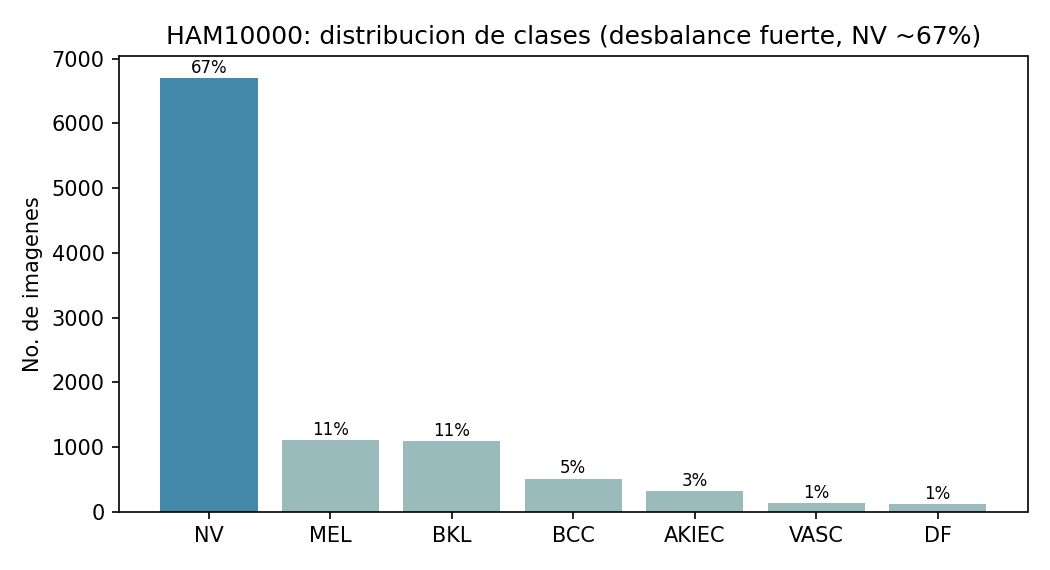
\includegraphics[width=0.7\textwidth]{F0_ham_dist.png}
  \caption{Distribución de clases en HAM10000. El fuerte predominio de la clase NV condiciona la
  elección de métricas y la interpretación de los resultados.}
  \label{fig:ham}
\end{figure}

Cabe adelantar un dato relevante para la Sección~\ref{sec:rediag}: los datos con los que se
\emph{entrena} la generación (SkinCoT) están organizados en $\sim$23 categorías clínicas y
\emph{no} presentan el sesgo NV/MEL de HAM; este hecho será clave al analizar por qué fallan los VLMs.

\subsection{Métricas y por qué se eligen}
\label{sec:metricas}
\paragraph{Clasificación.} Se reportan cuatro métricas. La \textbf{exactitud} (\emph{accuracy}) es la
fracción de aciertos; en esta tesina es poco informativa por sí sola debido al desbalance de HAM. El
\textbf{F1 ponderado} equilibra precisión y exhaustividad pero, al ponderar por frecuencia, también
queda dominado por la clase mayoritaria. El \textbf{F1 macro} promedia el F1 de cada clase sin ponderar,
de modo que penaliza tanto no detectar una clase rara (\emph{recall} bajo) como sobre-predecirla
(precisión baja). La métrica que se prioriza es la \textbf{sensibilidad macro} (promedio del
\emph{recall} por clase, sin ponderar): da el mismo peso a cada clase y, por lo tanto, \emph{mide
directamente si el modelo detecta las clases minoritarias}.

La razón de esa prioridad es concreta. Nevo (NV) es el $67\%$ del conjunto, así que un clasificador
trivial que responde ``nevo'' a todo obtiene \textbf{exactitud $0.669$} y F1 ponderado $0.537$ sin
reconocer una sola lesión maligna; su sensibilidad macro es $1/7 \approx 0.143$ (azar) y su F1 macro
$0.115$. No es un caso hipotético: Mini-VLM ajustado (Cuadro~\ref{tab:clasificacion}) llega a exactitud
$0.660$ con sensibilidad macro $0.141$, porque colapsa a nevo. En un problema así, un número alto de
exactitud puede no significar nada, y la sensibilidad macro lo expone de inmediato. Además, en este dominio
el error más caro es no detectar una clase rara y maligna (melanoma, carcinoma basocelular), que es
exactamente lo que el \emph{recall} por clase mide. El F1 macro se reporta como complemento porque la
sensibilidad macro sola no ve el costo inverso: un modelo que sobre-predice las clases raras sube su
sensibilidad a costa de falsos positivos masivos sobre nevo, y el F1 macro sí lo penaliza. Las dos se leen
juntas; cuando divergen, la diferencia indica justamente ese intercambio entre detectar y sobre-alertar.

\paragraph{Generación de reportes.} La evaluación tiene dos niveles. El \textbf{Nivel 1} (con
referencia) compara el reporte generado contra uno de referencia: BLEU-4, ROUGE-L, METEOR y CIDEr miden
solapamiento textual, y BERTScore mide similitud semántica. En este trabajo de experimentación, el Nivel 1 cuantifica
\emph{cuán parecido es el reporte generado a uno de referencia}, y solo puede aplicarse a
datasets que los traen (MM-Skin, SkinCoT); HAM no los tiene. Conviene precisar el origen de esas
referencias: las de MM-Skin provienen de libros de texto y las de SkinCoT las genera un pipeline de
modelos de lenguaje que luego \emph{certifican} dermatólogos (Sección~\ref{sec:datasets}). Es decir, el
Nivel 1 mide parecido contra un texto de referencia validado, no necesariamente redactado por un
especialista. El \textbf{Nivel 2} (sin
referencia) mide el contenido clínico directamente: \emph{clinical entity recall} (qué proporción de
categorías de términos dermatológicos aparece en el reporte; mide \emph{riqueza}) y \emph{diagnostic
consistency} (qué proporción de reportes menciona el diagnóstico correcto; mide \emph{fidelidad
diagnóstica}). En esta tesina, la \emph{diagnostic consistency} es la métrica más importante de
generación, porque captura lo que clínicamente más interesa: que el reporte acierte el diagnóstico.
\paragraph{Fidelidad diagnóstica no es validez clínica.} Conviene fijar desde acá qué afirma y qué no
afirma esta métrica, porque atraviesa todo el análisis de generación. La \emph{diagnostic consistency}
mide \textbf{fidelidad diagnóstica automática}: si el diagnóstico verdadero (o un sinónimo) aparece en el
texto. Está más cerca de lo clínicamente relevante que el solapamiento léxico, pero no verifica que la
descripción morfológica sea correcta para esa lesión, que no haya afirmaciones falsas junto al
diagnóstico correcto, ni que el reporte sea útil o seguro para quien lo lee. El \emph{clinical entity
recall}, por su parte, mide la presencia de términos, no su pertinencia. Ambas son \emph{proxies}. Por
eso, en este documento, ``fidelidad'' y ``consistencia'' se usan en ese sentido acotado, y
\textbf{ningún resultado se presenta como evidencia de utilidad ni de validez clínica}: establecerlas
requiere la evaluación de especialistas, que excede el alcance de esta experimentación.

% ============================================================
\section{Clasificación diagnóstica}
\label{sec:clasif}
% ============================================================
\subsection{Diseño del experimento}
\label{sec:clasif_diseno}
Se comparan tres familias de modelos (Figura~\ref{fig:tipos}) sobre el conjunto completo de HAM10000.

\begin{figure}[H]
\centering
\begin{tikzpicture}[
  box/.style={rectangle, rounded corners, draw, thick, align=center, minimum height=1.1cm, minimum width=3.4cm, font=\small},
  lbl/.style={font=\footnotesize\itshape, align=center}, >=Stealth]
  \node[box, draw=sup] (a) {CNN / ViT\\ \textbf{supervisado}};
  \node[box, draw=vlmgen, right=1.2cm of a] (b) {VLM \textbf{generativo}\\ (codif.\ + LLM)};
  \node[box, draw=vlcls, right=1.2cm of b] (c) {VL classifier\\ \textbf{CLIP-style}};
  \node[lbl, below=0.12cm of a] {imagen $\rightarrow$ logits\\ \emph{solo clasifica}};
  \node[lbl, below=0.12cm of b] {imagen+texto $\rightarrow$ texto\\ \emph{clasifica y genera}};
  \node[lbl, below=0.12cm of c] {similitud imagen--texto\\ \emph{solo clasifica}};
  \node[font=\scriptsize, below=1.05cm of a, text width=3.6cm, align=center] {DenseNet, ViT, ConvNeXt, Swin};
  \node[font=\scriptsize, below=1.05cm of b, text width=3.6cm, align=center] {LLaVA-Med, Mini-VLM};
  \node[font=\scriptsize, below=1.05cm of c, text width=3.6cm, align=center] {DermLIP (Derm1M)};
\end{tikzpicture}
\caption{Las tres familias de modelos. Un \emph{VL classifier} CLIP-style alinea un codificador de
imagen y uno de texto en un espacio común y clasifica por similitud, pero \emph{no} genera texto.}
\label{fig:tipos}
\end{figure}

\paragraph{Modelos supervisados (baseline).} DenseNet121, ViT-B/16, ConvNeXt-Tiny y Swin-Tiny, ajustados
por \emph{transfer learning} desde ImageNet (optimizador AdamW, \emph{cosine annealing}, \emph{early
stopping}, pérdida con pesos por clase para mitigar el desbalance). Producen directamente una
distribución sobre las 7 clases.

\paragraph{VLMs evaluados.} Se usaron dos VLMs generativos:
\begin{itemize}[leftmargin=1.6em]
  \item \textbf{LLaVA-Med 7B}~\cite{li2024llavamed}: codificador visual CLIP ViT-L/14 + modelo de
  lenguaje Mistral-7B, conectados por una proyección. Es un asistente biomédico general.
  \item \textbf{Mini-VLM}: codificador CLIP ViT-B/16 + modelo de lenguaje Phi-3.5, más pequeño.
\end{itemize}
Ambos son VLMs \emph{generativos}: producen \emph{texto}, no una distribución sobre clases. Para
clasificar con ellos se probaron cuatro estrategias (Figura~\ref{fig:zsvslik}):

\begin{enumerate}[leftmargin=1.6em]
  \item \textbf{Zero-shot por generación.} Se le da la imagen y un \emph{prompt} (``clasifica esta
  imagen en una de: MEL, NV, \dots'') y se \emph{parsea} la clase de su respuesta en texto libre. Su
  debilidad es el \emph{greedy trap}: la respuesta depende de la decodificación y a veces no contiene
  una clase válida (se marca como \emph{desconocido}).
  \item \textbf{Likelihood scoring.} En lugar de leer la respuesta generada, se calcula, para cada
  clase, la probabilidad que el modelo asigna a su \emph{nombre} (y sinónimos) dado la imagen y el
  \emph{prompt}, y se elige la de mayor probabilidad. Evita el \emph{greedy trap} y nunca produce
  ``desconocido''.
  \item \textbf{Chain-of-Thought (CoT).} Se le pide razonar paso a paso (describir rasgos, listar
  diferenciales) antes de concluir; se parsea el diagnóstico final.
  \item \textbf{Fine-tuning.} Se ajusta el modelo a la tarea con LoRA (\emph{Low-Rank Adaptation}, que
  entrena un pequeño conjunto de parámetros adicionales manteniendo congelado el resto), y luego se
  evalúa con \emph{likelihood} o CoT.
\end{enumerate}

\begin{figure}[H]
\centering
\begin{tikzpicture}[
  box/.style={rectangle, rounded corners, draw, align=center, minimum height=0.9cm, font=\footnotesize, inner sep=4pt},
  >=Stealth, node distance=0.55cm and 0.9cm]
  % zero-shot
  \node[box] (zimg) {imagen + \emph{prompt}};
  \node[box, right=of zimg, draw=vlmgen] (zgen) {VLM genera\\ texto libre};
  \node[box, right=of zgen] (zpar) {\emph{parser} $\rightarrow$\\ clase / ``desconocido''};
  \draw[->] (zimg)--(zgen); \draw[->] (zgen)--(zpar);
  \node[left=0.1cm of zimg, font=\scriptsize\bfseries] {(a) zero-shot};
  % likelihood
  \node[box, below=1.0cm of zimg] (limg) {imagen + \emph{prompt}};
  \node[box, right=of limg, draw=vlmgen] (lsc) {VLM puntúa $P(\text{nombre}_c \mid \text{img})$\\ para cada clase $c$};
  \node[box, right=of lsc] (lmax) {$\arg\max_c$\\ (sin ``desconocido'')};
  \draw[->] (limg)--(lsc); \draw[->] (lsc)--(lmax);
  \node[left=0.1cm of limg, font=\scriptsize\bfseries] {(b) likelihood};
\end{tikzpicture}
\caption{Dos formas de clasificar con un VLM generativo. (a) \emph{Zero-shot}: se lee la clase de la
respuesta en texto. (b) \emph{Likelihood scoring}: se elige la clase cuyo nombre el modelo considera más
probable dada la imagen; evita ambigüedades de la decodificación.}
\label{fig:zsvslik}
\end{figure}

\subsection{Resultados y comparación con el baseline}
El Cuadro~\ref{tab:clasificacion} y la Figura~\ref{fig:f1} muestran el resultado. Los clasificadores
supervisados rinden bien (Swin-Tiny~\cite{liu2021swin}: F1 = 0.882, sensibilidad macro 0.870). En
contraste, los VLMs generales \textbf{colapsan} en \emph{likelihood scoring} —la única estrategia
cuantificada en el Cuadro~\ref{tab:clasificacion}—: su sensibilidad macro ($0.137$--$0.181$) está al nivel
del azar ($1/7 \approx 0.143$). \emph{Chain-of-Thought} y \emph{zero-shot} por generación de texto no se
midieron con la misma métrica, pero la evidencia cualitativa (Figura~\ref{fig:colapso}) muestra el mismo
patrón de concentración en pocas clases.

\begin{table}[H]
  \centering
  \caption{Clasificación en HAM10000 (test). Supervisados vs VLMs médicos generales vs un VL classifier
  derm-especializado (DermLIP).}
  \label{tab:clasificacion}
  \begin{tabular}{llccc}
    \toprule
    \textbf{Enfoque} & \textbf{Modelo / método} & \textbf{Acc} & \textbf{F1} & \textbf{Sens.\ macro} \\
    \midrule
    \multirow{4}{*}{Supervisado}
      & DenseNet121      & 0.846 & 0.852 & 0.776 \\
      & ViT-B/16         & 0.858 & 0.862 & 0.797 \\
      & ConvNeXt-Tiny    & 0.827 & 0.861 & 0.849 \\
      & \textbf{Swin-Tiny} & \textbf{0.868} & \textbf{0.882} & \textbf{0.870} \\
    \midrule
    \multirow{4}{*}{VLM general}
      & LLaVA-Med likelihood (ZS) & 0.037 & 0.028 & 0.157 \\
      & Mini-VLM likelihood (ZS)  & 0.189 & 0.268 & 0.181 \\
      & LLaVA-Med likelihood (FT) & 0.179 & 0.198 & 0.137 \\
      & Mini-VLM likelihood (FT)  & 0.660 & 0.532 & 0.141 \\
    \midrule
    \multirow{2}{*}{VL derm-especializado}
      & DermLIP (zero-shot)    & 0.377 & 0.424 & 0.510 \\
      & DermLIP (linear-probe) & 0.741 & 0.762 & 0.739 \\
    \bottomrule
  \end{tabular}
\end{table}

\begin{figure}[H]
  \centering
  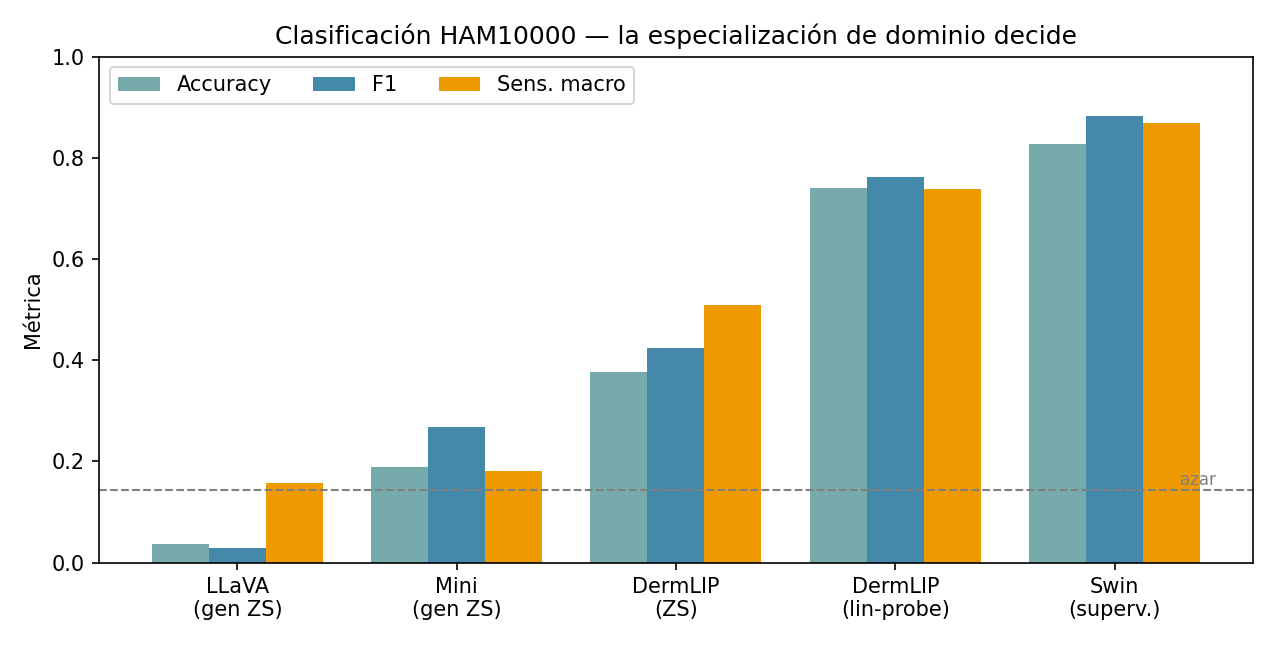
\includegraphics[width=0.9\textwidth]{F1_clasificacion.png}
  \caption{Clasificación HAM10000 por enfoque (línea punteada = azar en sensibilidad macro). Los VLMs
  generales quedan al nivel del azar; DermLIP discrimina incluso en zero-shot.}
  \label{fig:f1}
\end{figure}

\paragraph{Evidencia del colapso.} La métrica baja no es el único indicio. La Figura~\ref{fig:colapso}
muestra, para cada combinación VLM/método, la distribución de las clases \emph{predichas} frente a la
distribución verdadera. Cada combinación concentra casi todas sus predicciones en \emph{una sola} clase
—pero en una clase \emph{distinta} en cada caso (LLaVA en likelihood predice mayoritariamente MEL; Mini
en likelihood, NV; en CoT, MEL)—. En LLaVA con CoT, el 81\% de las respuestas no tiene etiqueta válida
(«desconocido»), y la figura lo muestra como VASC porque el código $-1$ indexó la última clase de la lista. Es decir, la predicción depende mucho más de la
configuración que de la lesión: el contenido de la imagen apenas la mueve, y el modelo tiende a responder
una clase casi constante.

\begin{figure}[H]
  \centering
  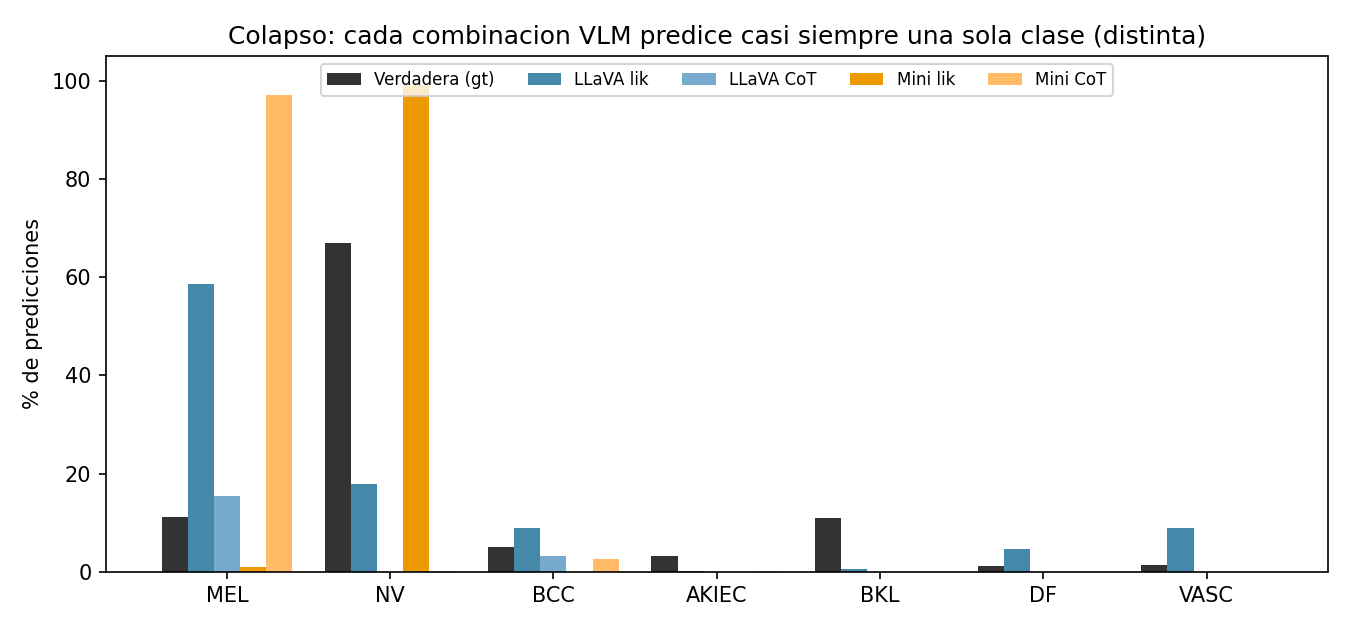
\includegraphics[width=0.95\textwidth]{F_colapso.png}
  \caption{Distribución de las clases predichas por cada combinación VLM (vs la distribución verdadera,
  en gris). Cada configuración colapsa hacia una clase distinta, señal de que la predicción no depende
  de la imagen.}
  \label{fig:colapso}
\end{figure}

\subsection{Comparación con el estado del arte}
\label{sec:clasif_sota}
El Cuadro~\ref{tab:sota_clasif} sitúa los resultados frente a la literatura, incluyendo modelos
supervisados del estado del arte (que en algunos casos alcanzan exactitudes superiores a las nuestras) y
VLMs. Se incluyen también nuestros VLMs tras \emph{fine-tuning} (FT): el caso de Mini-VLM es
ilustrativo —el ajuste eleva la exactitud a $0.66$ pero su sensibilidad macro sigue en $0.14$ (nivel de
azar)—, es decir, el modelo aprende a predecir la clase mayoritaria, no a discriminar. Es justamente el
fenómeno que la siguiente sección analiza.

La comparación también deja ver un \emph{gradiente de especialización}: los modelos derm-específicos
ajustados (PanDerm, un \emph{foundation model} con F1 ponderado $\approx 0.87$; los VLMs SkinVL ajustados
sobre dermatología, con sensibilidad macro $\approx 0.60$) recuperan capacidad de discriminación frente
a los VLMs generales (sensibilidad macro $\approx 0.14$), aunque sin alcanzar a los mejores
clasificadores supervisados. Esta comparación entre trabajos es \textbf{orientativa} —cada fila usa un
protocolo y un dataset distintos (nota del Cuadro~\ref{tab:sota_clasif})— y por sí sola no aísla la causa;
la evidencia más sólida de que la especialización de dominio, más que la mera escala o el carácter
``visión--lenguaje'', es lo que explica el desempeño viene del experimento \emph{controlado} con
\emph{embeddings} congelados de la Sección~\ref{sec:dermlip} (mismo clasificador clásico, misma
arquitectura base, solo cambia el preentrenamiento), donde el gradiente se reproduce sin las diferencias
de protocolo entre papers.

\begin{table}[H]
  \centering
  \caption{Comparación con el estado del arte en clasificación HAM10000 (7 clases). Los valores de los
  VLMs provienen de las evaluaciones sobre HAM10000 de los trabajos citados: Skin-R1 (Tabla~3, basada en
  \emph{prompts}, F1 macro) y MM-Skin (Tabla~4, \emph{fine-tuning} supervisado; su columna de
  sensibilidad es el \emph{recall} macro). ``---'' = no reportado.
  $^{\ast}$SkinSavvy2 se evalúa sobre un dataset aumentado derivado de HAM10000 (no el \emph{test}
  estándar) y reporta exactitud \emph{balanceada}. $^{\dagger}$PanDerm: F1 ponderado sobre HAM10000
  (7 clases) leído de la Fig.~2 del paper. Los protocolos de evaluación difieren entre trabajos, por lo
  que la comparación es orientativa. $^{\ddagger}$SkinVL-Pub/SkinVL-PubMM son los checkpoints
  \emph{publicados} por~\cite{zeng2025mmskin} (SOTA citado, evaluados aquí sobre HAM10000); no deben
  confundirse con SkinVL-MM, el generador de reportes de la misma familia que este trabajo integra al
  ensamble propio (Sección~\ref{sec:skinvl}, Cuadro~\ref{tab:skinvl}) — comparten arquitectura base pero
  son \emph{checkpoints} y evaluaciones distintas.}
  \label{tab:sota_clasif}
  \small
  \resizebox{\textwidth}{!}{%
  \begin{tabular}{llccc}
    \toprule
    \textbf{Modelo} & \textbf{Tipo} & \textbf{Acc} & \textbf{F1} & \textbf{Sens.\ macro} \\
    \midrule
    \multicolumn{5}{@{}l}{\itshape Estado del arte --- supervisados y \emph{foundation models}} \\
    EfficientNetB1+B5 (ens.)~\cite{SkinHealthMate2024} & CNN (FT) & \textbf{0.930} & \textbf{0.930} & --- \\
    PanDerm (foundation ViT)$^{\dagger}$~\cite{yan2025panderm} & Foundation (FT) & --- & 0.870 & --- \\
    Swin-Transformer$^{\ast}$~\cite{SkinSavvy22025} & ViT (FT) & 0.780 & 0.793 & --- \\
    \multicolumn{5}{@{}l}{\itshape Estado del arte --- VLMs} \\
    Skin-R1 (Qwen2.5-VL-7B + RL)~\cite{liu2025skinr1} & VLM (FT+RL) & 0.747 & 0.404 & --- \\
    LLaVA-Med-7B~\cite{liu2025skinr1} & VLM (ZS) & 0.230 & 0.125 & --- \\
    SkinVL-Pub$^{\ddagger}$ (LLaVA-Med+LoRA)~\cite{zeng2025mmskin} & VLM (FT) & 0.793 & --- & 0.602 \\
    SkinVL-PubMM$^{\ddagger}$ (LLaVA-Med+LoRA)~\cite{zeng2025mmskin} & VLM (FT) & 0.790 & --- & 0.626 \\
    \midrule
    \multicolumn{5}{@{}l}{\itshape Este trabajo} \\
    Swin-Tiny & Supervisado & 0.868 & 0.882 & \textbf{0.870} \\
    LLaVA-Med likelihood & VLM (ZS) & 0.037 & 0.028 & 0.157 \\
    Mini-VLM likelihood & VLM (ZS) & 0.189 & 0.268 & 0.181 \\
    LLaVA-Med likelihood & VLM (FT) & 0.179 & 0.198 & 0.137 \\
    Mini-VLM likelihood & VLM (FT) & 0.660 & 0.532 & 0.141 \\
    DermLIP & VL derm (ZS) & 0.377 & 0.424 & 0.510 \\
    DermLIP & VL derm (lin-probe) & 0.741 & 0.762 & 0.739 \\
    \bottomrule
  \end{tabular}%
  }
\end{table}

\subsection{¿Por qué fallan los VLMs generales? Re-diagnóstico}
\label{sec:rediag}
Conviene primero situar nuestros resultados frente a la literatura, porque lejos de contradecirla, la
\textbf{corroboran}. El trabajo de Skin-R1~\cite{liu2025skinr1} evalúa a estos mismos VLMs sobre
HAM10000 (7 clases) y observa el mismo fenómeno que nosotros: reporta que LLaVA-Med-7B obtiene un F1
muy bajo ($\approx 0.12$, Cuadro~\ref{tab:sota_clasif}) y lo atribuye explícitamente a un
\emph{``fuerte sesgo hacia la clase mayoritaria (benigna), con 5563 de 8390 predicciones''}; y describe
que otro VLM (MedGemma) colapsa, en cambio, hacia una clase \emph{rara}. Es exactamente el patrón de la
Figura~\ref{fig:colapso}: cada VLM concentra sus predicciones en una clase distinta. No hay, por lo
tanto, contradicción: tanto nuestros experimentos como la literatura encuentran que los VLMs generales
fallan en la clasificación de grano fino de HAM10000.

\paragraph{Sobre las diferencias de exactitud.} Nuestra exactitud ($0.037$) es aún más baja que la de
esos baselines porque (a) usamos \emph{likelihood scoring} en lugar de generación con parseo, y
(b) nuestra configuración colapsa hacia una clase \emph{minoritaria} (MEL), mientras que un colapso
hacia la clase mayoritaria (NV, $67\%$) produciría una exactitud alta sin discriminar —de hecho,
nuestro propio Mini-VLM alcanza $66\%$ de exactitud colapsando a NV, con sensibilidad macro de apenas
$0.14$—. Por eso la \emph{exactitud} es engañosa y la \textbf{sensibilidad macro} (cercana al azar en
todas las variantes) es la métrica que revela el colapso de fondo.

Establecido que el fenómeno es real y compartido con la literatura, se investigó su causa. La primera
hipótesis —el \emph{desbalance de entrenamiento}— se descartó con cuatro evidencias: (i) el colapso 
aparece en \emph{zero-shot}, antes de todo fine-tuning; (ii) los
datos de entrenamiento del generador no están sesgados a NV/MEL; (iii) cada configuración colapsa a una
clase \emph{distinta} (Figura~\ref{fig:colapso}), incompatible con un sesgo de frecuencia; y (iv) al
evaluar sobre \emph{foto clínica} el VLM \emph{tampoco} discrimina, descartando un problema específico
de la dermatoscopía. \textbf{Conclusión:} el bajo rendimiento es una limitación general de
estos VLMs para la discriminación dermatológica de grano fino: sus predicciones están guiadas por el prior
del lenguaje (qué nombre de clase es más ``esperable'' dado el \emph{prompt}) más que por el contenido
visual. Esto se verificó \textbf{directamente} midiendo $P(\text{clase}\mid\text{prompt})$ con la imagen
reemplazada por una imagen gris neutra (sin contenido visual): privados de la imagen, ambos VLMs siguen
prediciendo con aplomo y \textbf{colapsan al $100\%$ en una única clase fija} —Mini-VLM a melanoma,
LLaVA-Med a dermatofibroma— sin abstenerse nunca, con una exactitud igual a la mera prevalencia de esa clase
($0.111$ y $0.011$). Al reincorporar la imagen las predicciones apenas se dispersan (Mini-VLM pasa de $1$ a
$2$ clases y de exactitud $0.111$ a $0.189$; LLaVA-Med de $1$ a $5$ clases), confirmando que la señal visual
está presente pero es \emph{demasiado débil para discriminar}: el prior domina. La evidencia motiva
incorporar un modelo \emph{especializado en el dominio}.

\paragraph{El desbalance tampoco limita al clasificador supervisado.} Para cerrar la hipótesis del
desbalance también del lado del \emph{clasificador}, se entrenó Swin-Tiny cuatro veces variando
\emph{únicamente} la función de pérdida y dejando fijo todo lo demás (arquitectura, augmentación,
hiperparámetros, semilla), de modo que cualquier diferencia se atribuya a cómo la pérdida trata a las
clases minoritarias. Las cuatro variantes son: \emph{entropía cruzada} (CE) simple, que no distingue
clases; \emph{CE con pesos por clase}, que multiplica el error de cada clase por un peso inverso a su
frecuencia (castiga más equivocarse en una clase rara); \emph{Focal Loss}, que baja el peso de los
ejemplos ya bien clasificados para concentrarse en los difíciles; y \emph{Balanced Softmax}, que corrige
el sesgo de frecuencia dentro del propio softmax (Cuadro~\ref{tab:desbalance}). La métrica de interés es
la \textbf{sensibilidad macro} —promedio no ponderado del recall por clase—, porque le da el mismo peso a
una clase rara que a una frecuente y es, por tanto, la que un método de re-balanceo debería mejorar. Para
que la conclusión no dependa de una sola arquitectura, el experimento se repitió en \textbf{tres modelos}:
Swin-Tiny (transformer), ConvNeXt-Tiny (CNN moderno) y DenseNet121 (CNN clásico) (Cuadro~\ref{tab:desbalance}).

El resultado es consistente: la \textbf{CE simple, sin ningún manejo del desbalance, es la mejor opción
global} en las tres (gana las tres métricas en Swin —sensibilidad macro $0.887$— y en DenseNet, y domina
exactitud y F1-w en ConvNeXt). Los métodos de re-balanceo no compensan: las \emph{class-weights}
\emph{empeoran} en las tres arquitecturas (Swin $0.923\to0.795$ de exactitud, ConvNeXt $0.912\to0.691$,
DenseNet $0.876\to0.563$), y aunque en ConvNeXt la \emph{Focal Loss} sube apenas la sensibilidad macro
($0.824\to0.842$), lo hace a costa de \emph{once puntos} de exactitud ($0.912\to0.803$) —una mejora que no
es gratuita—. La arquitectura y la augmentación ya bastan para discriminar
las clases minoritarias de HAM: el desbalance no es el cuello de botella del clasificador, y por lo tanto
tampoco explica el colapso de los VLMs.

El \emph{porqué} de este comportamiento es coherente con esa lectura. Los métodos de re-balanceo corrigen
un sesgo hacia la clase mayoritaria desplazando la frontera de decisión en favor de las raras. Pero ese
sesgo, en este caso, \textbf{ya estaba compensado} por la augmentación fuerte del \emph{recipe} moderno:
la CE simple alcanza sensibilidad macro $0.887$, es decir, el modelo ya reconoce bien las clases
minoritarias. Al aplicar entonces una corrección adicional, esta no elimina un sesgo sino que
\emph{introduce el opuesto}: el modelo pasa a sobre-predecir clases raras, generando falsos positivos
masivos sobre el nevo —que concentra el $67\%$ del conjunto—, lo que derrumba la exactitud ($0.923 \to
0.795$ en Swin, $0.876 \to 0.563$ en DenseNet) sin ganar sensibilidad macro a cambio. Cuanto más agresiva
la corrección, peor el resultado: las \emph{class-weights}, que reponderan por frecuencia inversa y por
tanto amplifican más las clases de menor prevalencia, son las que más daño hacen en las tres arquitecturas.
En otras palabras, el re-balanceo falla aquí no por estar mal implementado, sino porque \textbf{corrige un
problema que el modelo ya había resuelto por otra vía}.

\emph{Una aclaración de cronología.} Los clasificadores \emph{headline} (Cuadro~\ref{tab:clasificacion})
se entrenaron con \emph{pesos por clase}, una decisión previa a este análisis. El hallazgo de que la CE
simple los iguala o supera es \emph{posterior} —surge de este experimento de re-balanceo—, de modo que los
números \emph{headline} reportados son, si acaso, \emph{conservadores}: un Swin con CE simple alcanza aún
mayor sensibilidad macro ($0.887$ frente a $0.870$). No se re-generó toda la comparación con CE para no
mezclar corridas; la conclusión relevante —que el manejo del desbalance no ayuda— no cambia.

\begin{table}[H]
  \centering
  \caption{Manejo explícito del desbalance sobre tres arquitecturas (Swin-Tiny, transformer; ConvNeXt-Tiny,
  CNN moderno; DenseNet121, CNN clásico), mismo recipe, variando solo la loss; test HAM con
  \emph{test-time augmentation} (TTA: se promedia la predicción sobre varias vistas aumentadas). En las
  tres, el re-balanceo no compensa a la CE simple.}
  \label{tab:desbalance}
  \begin{tabular}{llccc}
    \toprule
    \textbf{Modelo} & \textbf{Pérdida} & \textbf{Acc} & \textbf{F1-w} & \textbf{Sens.\ macro} \\
    \midrule
    \multirow{4}{*}{Swin-Tiny}
      & CE simple (sin manejo) & \textbf{0.923} & \textbf{0.923} & \textbf{0.887} \\
      & Balanced Softmax       & 0.856 & 0.872 & 0.857 \\
      & Focal Loss ($\gamma=2$) & 0.820 & 0.843 & 0.857 \\
      & CE + class-weights     & 0.795 & 0.816 & 0.809 \\
    \midrule
    \multirow{4}{*}{ConvNeXt-Tiny}
      & CE simple (sin manejo) & \textbf{0.912} & \textbf{0.910} & 0.824 \\
      & Focal Loss ($\gamma=2$) & 0.803 & 0.840 & \textbf{0.842} \\
      & Balanced Softmax       & 0.783 & 0.826 & 0.834 \\
      & CE + class-weights     & 0.691 & 0.753 & 0.808 \\
    \midrule
    \multirow{4}{*}{DenseNet121}
      & CE simple (sin manejo) & \textbf{0.876} & \textbf{0.870} & \textbf{0.738} \\
      & Balanced Softmax       & 0.629 & 0.701 & 0.735 \\
      & CE + class-weights     & 0.563 & 0.652 & 0.735 \\
      & Focal Loss ($\gamma=2$) & 0.564 & 0.658 & 0.725 \\
    \bottomrule
  \end{tabular}
\end{table}

\subsection{La especialización de dominio recupera la discriminación}
\label{sec:dermlip}
\paragraph{Qué es DermLIP.} DermLIP~\cite{yan2025derm1m} es un \emph{VL classifier} de tipo CLIP: un
codificador de imagen (ViT-B/16) y un codificador de texto entrenados de forma \emph{contrastiva} para
quedar alineados en un espacio común, de modo que la imagen y la descripción correcta de su diagnóstico
queden ``cerca''. A diferencia de un VLM generativo, no produce texto: clasifica midiendo la
\emph{similitud} entre la imagen y el nombre de cada clase. Su pre-entrenamiento usó Derm1M
($\sim$1M pares imagen--texto dermatológicos con ontología clínica), lo que le da especialización de
dominio.

\paragraph{Evidencia de que recupera la discriminación.} Se evaluó de dos formas: \emph{zero-shot}
(clasificando por similitud, sin entrenarlo en HAM) y \emph{linear-probe} (congelando el codificador y
entrenando solo un clasificador lineal sobre sus \emph{embeddings}, lo que mide la calidad de las
representaciones). Los resultados sostienen la afirmación de tres maneras concretas:
\begin{itemize}[leftmargin=1.6em]
  \item \textbf{Sensibilidad macro muy por encima del azar}: $0.510$ en zero-shot (vs $\approx 0.14$ de
  los VLMs generales y $0.143$ del azar), y $0.739$ con linear-probe (Cuadro~\ref{tab:clasificacion}).
  \item \textbf{No colapsa}: predice las 7 clases con sensibilidades por clase razonables (no concentra
  todo en una), a diferencia de la Figura~\ref{fig:colapso}.
  \item \textbf{Generaliza entre dominios de imagen} (Cuadro~\ref{tab:dermlip_dominio}): discrimina
  tanto en dermatoscopía como en foto clínica, lo que confirma que el factor decisivo es la
  especialización y no la modalidad.
\end{itemize}
Es importante ser preciso sobre el sentido de ``recuperar la discriminación'': en sus modos
\emph{nativos} (zero-shot, linear-probe), DermLIP no supera al mejor clasificador supervisado
(Swin-Tiny: Acc $0.868$ / F1 $0.882$ / sens.\ macro $0.870$); lo que hace es \emph{romper el colapso} de
los VLMs generales y alcanzar, con un simple linear-probe, un F1 ($0.762$) cercano al supervisado. Con
una cabeza no lineal trivial sobre sus \emph{embeddings} congelados (SVM-RBF, se detalla más abajo), el
panorama es más matizado: ese pipeline alcanza Acc $0.881$ y F1 $0.881$ —ambos \emph{por encima} de
Swin— pero sensibilidad macro $0.788$, \textbf{por debajo} de Swin ($0.870$), la métrica que la
Sección~\ref{sec:clasif_diseno} prioriza por el desbalance de clases. Es decir: en las métricas
agregadas (Acc, F1) un SVM barato sobre \emph{embeddings} de DermLIP iguala o supera al supervisado
fine-tuneado; en la métrica prioritaria para este problema desbalanceado, sigue por debajo. En ningún
caso el problema era ``usar un modelo visión--lenguaje'' sino usar uno \emph{no especializado}.

\begin{table}[H]
  \centering
  \caption{DermLIP por dominio de imagen (7 clases HAM). La discriminación se mantiene en dermatoscopía
  y en foto clínica.}
  \label{tab:dermlip_dominio}
  \begin{tabular}{llccc}
    \toprule
    \textbf{Dominio} & \textbf{Modo} & \textbf{Acc} & \textbf{F1} & \textbf{Sens.\ macro} \\
    \midrule
    HAM (dermatoscopía) & zero-shot    & 0.377 & 0.424 & 0.510 \\
    HAM (dermatoscopía) & linear-probe & 0.741 & 0.762 & 0.739 \\
    SkinCAP (clínica)   & zero-shot    & 0.386 & 0.375 & 0.454 \\
    \bottomrule
  \end{tabular}
\end{table}

\paragraph{¿Por qué DermLIP recupera la discriminación?} A diferencia de los VLMs generativos —que se
entrenan para \emph{predecir el siguiente token} sobre corpus biomédicos amplios—, DermLIP es un modelo
\emph{contrastivo} (estilo CLIP) preentrenado sobre Derm1M~\cite{yan2025derm1m}: $\sim$1M de pares
imagen--texto \emph{específicos de dermatología} alineados con una ontología clínica. El objetivo
contrastivo alinea explícitamente la representación visual con la textual de cada concepto, de modo que
las clases de lesiones quedan \emph{separadas en el espacio de embeddings} antes de cualquier ajuste
supervisado. Esto explica por qué discrimina en zero-shot donde los VLMs generales colapsan: no es la
capacidad ``visión--lenguaje'' en abstracto lo que ayuda, sino el \emph{preentrenamiento especializado de
dominio} —a gran escala y con supervisión contrastiva— lo que produce representaciones útiles para el
grano fino dermatológico, en línea con la tendencia actual de los \emph{foundation models} médicos.

\paragraph{Evidencia: la representación ya separa las clases.} Un modelo profundo hace dos cosas: primero
transforma la imagen en un vector de características (el \emph{embedding}) y luego una capa final decide la
clase a partir de ese vector. Para separar ambos aportes se hizo un experimento de \emph{linear probing}:
se congela el modelo preentrenado —no se ajusta ni un peso—, se extrae el embedding de cada imagen y sobre
esos vectores fijos se entrenan clasificadores \emph{clásicos} y livianos (SVM-RBF, Random Forest,
regresión logística, todos con \texttt{class\_weight=balanced}). Si esos clasificadores simples ya
aciertan, la información discriminante está en el embedding; si no, hace falta que la red aprenda
representaciones nuevas. Sobre \emph{embeddings} de DermLIP, el \textbf{SVM-RBF es el mejor clásico}
(Acc $0.881$ / F1 $0.881$ / sens.\ macro $0.788$), seguido por regresión logística ($0.815$/$0.823$/$0.717$);
\textbf{Random Forest queda atrás} (Acc $0.818$ / F1 $0.794$ / sens.\ macro $0.550$), penalizado por la
alta dimensión del embedding. El SVM-RBF supera al \emph{linear-probe} reportado antes (F1 $0.762$,
Cuadro~\ref{tab:clasificacion}): el linear-probe es un clasificador \emph{lineal} (regresión logística sin
balanceo), mientras que el SVM con \emph{kernel} RBF captura estructura \emph{no lineal} del espacio de
embeddings. La diferencia ($0.762 \to 0.881$) indica que las clases ya están \emph{casi} separadas
linealmente y \emph{completamente} separables con una frontera no lineal simple —es decir, la
información discriminante está en la representación, no falta aprenderla—. La misma familia de
clasificadores sobre una representación \emph{genérica} (Swin preentrenado en ImageNet, congelado) rinde
bastante menos —SVM-RBF sens.\ macro $0.579$, Random Forest colapsa a $0.163$—: es decir, las clases de
lesiones ya están \emph{separadas en el espacio de embeddings derm-especializado}, y no tanto en el
genérico: lo determinante es la especialización de dominio de la \emph{representación}, no la
arquitectura ni el clasificador elegido sobre ella.

\subsection{Robustez de las probabilidades y significancia estadística}
\label{sec:calib}
Dos preguntas de rigor completan la evaluación de clasificación: ¿son confiables las \emph{probabilidades}
de los clasificadores?, y ¿son \emph{significativas} las diferencias observadas?

\paragraph{Qué miden estas métricas.} Para la \emph{calibración} se agrupan las predicciones en
\emph{bins} según su confianza (la probabilidad máxima que asigna el modelo) y, en cada bin, se compara
la confianza promedio con la exactitud real. El \textbf{ECE} (\emph{Expected Calibration Error}) es el
promedio —ponderado por la cantidad de muestras de cada bin— de esa brecha $|\text{exactitud}-\text{
confianza}|$; el \textbf{MCE} (\emph{Maximum Calibration Error}) es la brecha \emph{máxima} entre bins; y
el \textbf{Brier score} es el error cuadrático medio entre la distribución de probabilidad predicha y la
etiqueta real (0 = perfecto). En los tres, menor es mejor. Para la \emph{significancia}, el test de
\textbf{McNemar} compara dos modelos sobre las \emph{mismas} imágenes contando solo los casos
\emph{discordantes} (uno acierta y el otro no): si esos desacuerdos se reparten muy desigualmente, la
diferencia entre los modelos no es atribuible al azar (un $p$ bajo).

\paragraph{Calibración.} Un clasificador puede tener buena exactitud pero probabilidades mal calibradas
—afirmar, por ejemplo, 99\% de confianza y acertar mucho menos—, lo cual es peligroso en medicina. Se
midió el \emph{Expected Calibration Error} (ECE), el \emph{Maximum Calibration Error} (MCE) y el
\emph{Brier score} sobre el test de HAM (Cuadro~\ref{tab:calib}, Figura~\ref{fig:calib}). El resultado es
matizado: los clasificadores están mal calibrados (ECE $0.19$--$0.39$), pero \emph{en la dirección
opuesta a la temida}: son \textbf{sub-confiados}, no sobre-confiados. Swin, por ejemplo, tiene confianza
media $0.42$ pero exactitud $0.795$: cuando reporta confianzas en torno al $40\%$ en realidad acierta
$\sim$80\% (su curva queda \emph{por encima} de la diagonal en la Figura~\ref{fig:calib}). Además, \emph{a mayor
exactitud, peor calibración}: los mejores modelos (Swin, ConvNeXt) producen las probabilidades más
difusas, efecto plausiblemente atribuible a la regularización agresiva del \emph{recipe} de entrenamiento
moderno (aumentaciones fuertes, \emph{label smoothing}), que suaviza la salida del \emph{softmax}
independientemente del \emph{test-time augmentation} —estas exactitudes se miden \emph{single-view}, sin
TTA (nota del Cuadro~\ref{tab:calib})—. La implicancia es que la probabilidad cruda no sirve como estimador de certeza sin
calibrar previamente.

\begin{table}[H]
  \centering
  \caption{Calibración de los clasificadores supervisados en HAM (test, $n=1503$). ECE/MCE en $[0,1]$;
  Brier multiclase en $[0,2]$. Menor es mejor. Todos sub-confiados (exactitud $>$ confianza media).
  \emph{Nota de protocolo:} estas exactitudes se computaron \emph{single-view} (sin TTA) sobre los
  checkpoints \emph{modern} disponibles con probabilidades guardadas, por lo que son más bajas que las
  \emph{headline} del Cuadro~\ref{tab:clasificacion} (con TTA y, en Swin/ConvNeXt, el punto óptimo del
  barrido); lo relevante aquí es la calibración \emph{relativa}, no la exactitud absoluta.}
  \label{tab:calib}
  \begin{tabular}{lcccc}
    \toprule
    \textbf{Modelo} & \textbf{Acc} & \textbf{ECE}$\downarrow$ & \textbf{MCE}$\downarrow$ & \textbf{Brier}$\downarrow$ \\
    \midrule
    DenseNet121   & 0.590 & \textbf{0.188} & \textbf{0.289} & 0.606 \\
    ViT-B/16      & 0.668 & 0.273 & 0.397 & 0.623 \\
    Swin-Tiny     & 0.795 & 0.380 & 0.595 & 0.575 \\
    ConvNeXt-Tiny & 0.819 & 0.393 & 0.598 & \textbf{0.555} \\
    \bottomrule
  \end{tabular}
\end{table}

\begin{figure}[H]
  \centering
  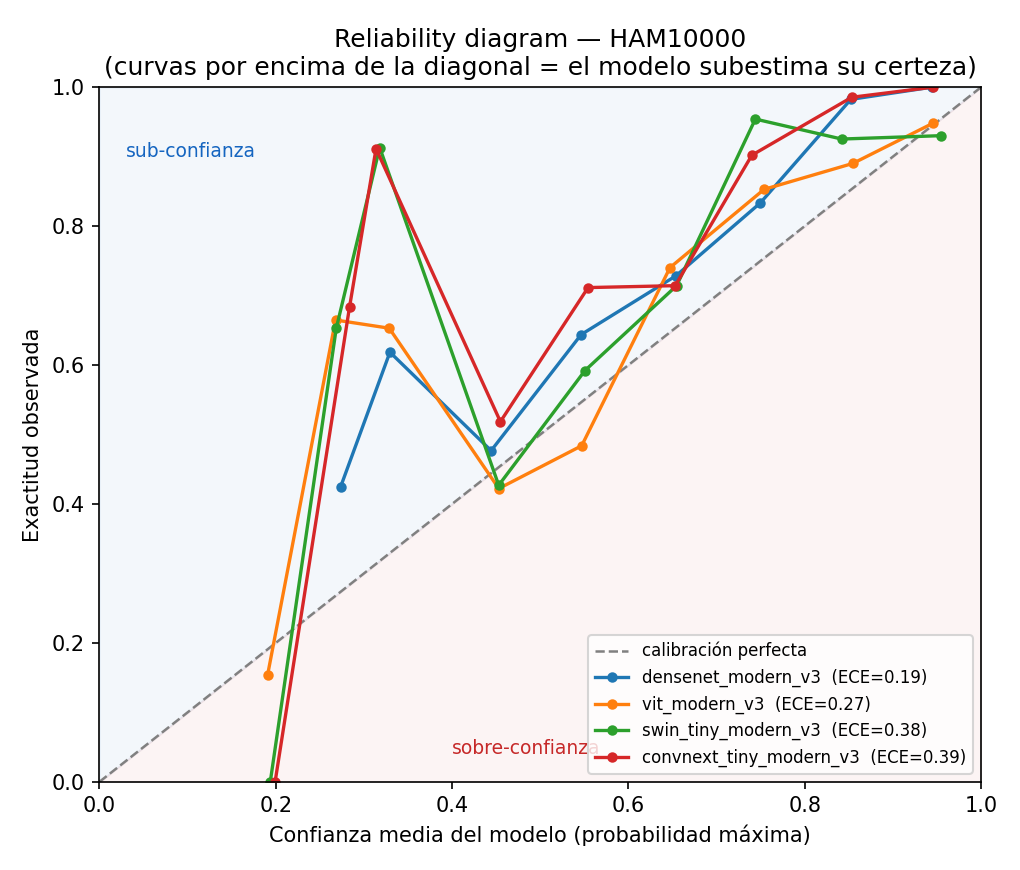
\includegraphics[width=\textwidth]{P01_calibration.png}
  \caption{Reliability diagram: exactitud observada vs.\ confianza media del modelo, una curva por
  clasificador (ECE entre paréntesis). Un modelo perfectamente calibrado seguiría la diagonal; las curvas
  quedan \emph{por encima} de ella (zona azul), es decir, los modelos \emph{subestiman} su certeza
  —``dicen'' menos confianza de la que su exactitud justifica—.}
  \label{fig:calib}
\end{figure}

\paragraph{Significancia estadística.} Para verificar que el orden observado no es ruido se calcularon
intervalos de confianza \emph{bootstrap} (95\%, 2000 remuestreos) y el test de \emph{McNemar} pareado
sobre las 1503 imágenes de test. El gradiente de especialización es \textbf{estadísticamente robusto}:
los IC de sensibilidad macro no se solapan entre Swin ($[0.77,0.85]$), DermLIP ($[0.46,0.56]$) y los VLMs
generales, y todas las diferencias por pares son significativas (McNemar $p<0.001$). Más aún, el colapso
de los VLMs generales queda confirmado con rigor bajo el protocolo \emph{zero-shot por generación}
(respuesta en texto libre, parseada a clase): el IC de sensibilidad macro de Mini-VLM es
$[0.137,0.152]$ y el de LLaVA-Med $[0.145,0.168]$, ambos \emph{abrazando el nivel de azar}
($1/7=0.143$) —es decir, estadísticamente indistinguibles del azar—. Este protocolo es distinto del
\emph{likelihood scoring} del Cuadro~\ref{tab:clasificacion} (donde Mini-VLM ZS alcanza sens.\ macro
$0.181$): ambos colapsan, pero no son el mismo número y no deben leerse como IC el uno del otro.

McNemar y los IC anteriores operan sobre la exactitud global; para contrastar el desempeño
\emph{por clase} —donde el desbalance pesa— se aplicó además un \textbf{test de Wilcoxon de rangos con
signo} sobre el \emph{recall} de las 7 clases, pareado por clase entre cada par de modelos
(Cuadro~\ref{tab:wilcoxon}). La ventaja de Swin-Tiny es significativa frente a los tres modelos
visión--lenguaje ($p \le 0.031$), con diferencias medianas de recall de $+0.24$ sobre DermLIP zero-shot y
de $+0.73$--$0.79$ sobre los VLMs generales. En cambio, \textbf{Mini-VLM y LLaVA-Med son indistinguibles
entre sí} ($p=1.00$, diferencia mediana $0.00$): ambos colapsan por igual, sin que ninguno domine al otro
en ninguna clase. DermLIP se separa de LLaVA-Med ($p=0.047$) pero no alcanza significancia frente a
Mini-VLM ($p=0.109$) con solo 7 pares, la limitación esperable de un test no paramétrico sobre tan pocas
observaciones.

\begin{table}[H]
  \centering
  \caption{Test de Wilcoxon de rangos con signo sobre el \emph{recall} por clase (7 pares, uno por clase de
  HAM10000), pareado entre modelos. ``Dif.\ mediana'' es la mediana de la diferencia de recall a favor del
  primer modelo. Complementa a McNemar, que compara aciertos globales pero no diferencias por clase.
  En negrita, los contrastes significativos ($p<0.05$).}
  \label{tab:wilcoxon}
  \begin{tabular}{lcc}
    \toprule
    \textbf{Comparación (recall por clase)} & \textbf{Dif.\ mediana} & \textbf{$p$} \\
    \midrule
    Swin-Tiny vs.\ DermLIP (ZS)       & $+0.235$ & \textbf{0.016} \\
    Swin-Tiny vs.\ Mini-VLM (ZS)      & $+0.794$ & \textbf{0.031} \\
    Swin-Tiny vs.\ LLaVA-Med (ZS)     & $+0.733$ & \textbf{0.031} \\
    DermLIP (ZS) vs.\ LLaVA-Med (ZS)  & $+0.329$ & \textbf{0.047} \\
    DermLIP (ZS) vs.\ Mini-VLM (ZS)   & $+0.471$ & 0.109 \\
    Mini-VLM (ZS) vs.\ LLaVA-Med (ZS) & $0.000$  & 1.000 \\
    \bottomrule
  \end{tabular}
\end{table}

\subsection{Robustez a condiciones de adquisición}
\label{sec:robustez}
Un clasificador entrenado sobre HAM10000 puede degradarse por dos vías al usarse en el entorno real:
porque cambia la \emph{población} de pacientes o porque cambia la \emph{calidad de imagen} de la cámara.
Ambas se evaluaron por separado.

\paragraph{Cambio de población (HIBA).} Se re-evaluaron los clasificadores —sin reentrenar— sobre
\textbf{HIBA} (Sección~\ref{sec:datasets}): $1616$ imágenes ($1270$ dermatoscópicas y $346$ clínicas) de pacientes argentinos con
fototipos III--VI, una población distinta a la de HAM10000 (mayoritariamente europea). Es una prueba
\emph{out-of-distribution} (OOD): mide cuánto cae el modelo cuando la piel y las condiciones de
adquisición no coinciden con las del entrenamiento.

\emph{Cómo se comparan HAM y HIBA (espacio diagnóstico).} La comparación se hace bajo el \textbf{mismo
espacio de 7 clases} de HAM10000. El mapeo de etiquetas HIBA$\to$HAM es \textbf{1:1 para 6 de las 7
categorías}; la única salvedad es el carcinoma espinocelular (SCC), que HAM no tiene como clase propia y se
\textbf{mapea a AKIEC} ($158$ imágenes afectadas), introduciendo algo de ruido de anotación en esa clase.
No se eliminan clases: todas las imágenes de HIBA se evalúan contra las 7 clases de HAM. Por eso es
importante ser cauto en la lectura: la caída puede provenir \emph{tanto} del cambio de población y de
equipo (\emph{domain shift} real) \emph{como} de esas diferencias de anotación/composición de clases —no
son totalmente separables con estos datos—.

Con esa salvedad, todos los modelos pierden entre $27$ y $40$ puntos de exactitud al pasar de HAM10000 a
HIBA (Swin-Tiny $\approx 0.87 \to 0.58$), un \emph{domain shift} marcado. Es la limitación más seria para
el despliegue clínico y justifica la evaluación de robustez que sigue.

\paragraph{Cambio de calidad de imagen.}
Se probaron cuatro perturbaciones —compresión JPEG, ruido gaussiano, desenfoque gaussiano y bajada de
resolución—, cada una en cinco \textbf{niveles de severidad} crecientes (sev1$\to$sev5). \emph{Cómo se
aplican, para que quede claro:} cada perturbación se aplica \textbf{por separado} (no se combinan entre
sí) y de forma \textbf{determinística} (no aleatoria): fijado el tipo y el nivel, se toma \emph{todo} el
test de HAM10000 ($n=1503$) y se le aplica ese único filtro con ese único parámetro, generando una
\emph{versión degradada completa} del test; luego se vuelve a correr el clasificador sobre ella y se mide
la sensibilidad macro. Es decir, se evalúan $4 \times 5 = 20$ versiones del conjunto de test (más el
original sin perturbar), una por cada combinación (perturbación, nivel). El parámetro de cada nivel varía
de forma monótona: calidad JPEG de $70$ a $5$, desviación del ruido $\sigma$ de $8$ a $64$, radio de
desenfoque de $1$ a $6$~px, y factor de resolución de $0.75$ a $0.15$ (se reduce la imagen y se re-escala
al tamaño original, perdiendo detalle). sev1 simula una degradación apenas perceptible y sev5 una imagen
muy dañada; la Figura~\ref{fig:robustez_ej} lo ilustra sobre dos imágenes de ejemplo. Lo relevante es la
\emph{degradación relativa}: el baseline se mide aquí \emph{single-view} (sin TTA), por lo que la
sensibilidad macro sin perturbar ($0.74$) es algo menor que la \emph{headline} con TTA ($0.87$).

Tres observaciones: (i) el \textbf{ruido} es la perturbación
más dañina —la sensibilidad macro de Swin cae de $0.74$ a $\approx 0.38$ ya con ruido moderado—; (ii) la
\textbf{resolución} es lo más tolerado (se mantiene $\approx 0.53$ aun con degradación severa: la
clasificación dermatoscópica no depende del detalle fino de píxel); y (iii) la degradación es
\emph{gradual} —a perturbación leve los modelos se mantienen sólidos ($0.65$–$0.83$), sin caer al azar
salvo bajo ruido o JPEG extremos—. ConvNeXt-Tiny resulta algo más robusto que Swin.

\begin{figure}[H]
  \centering
  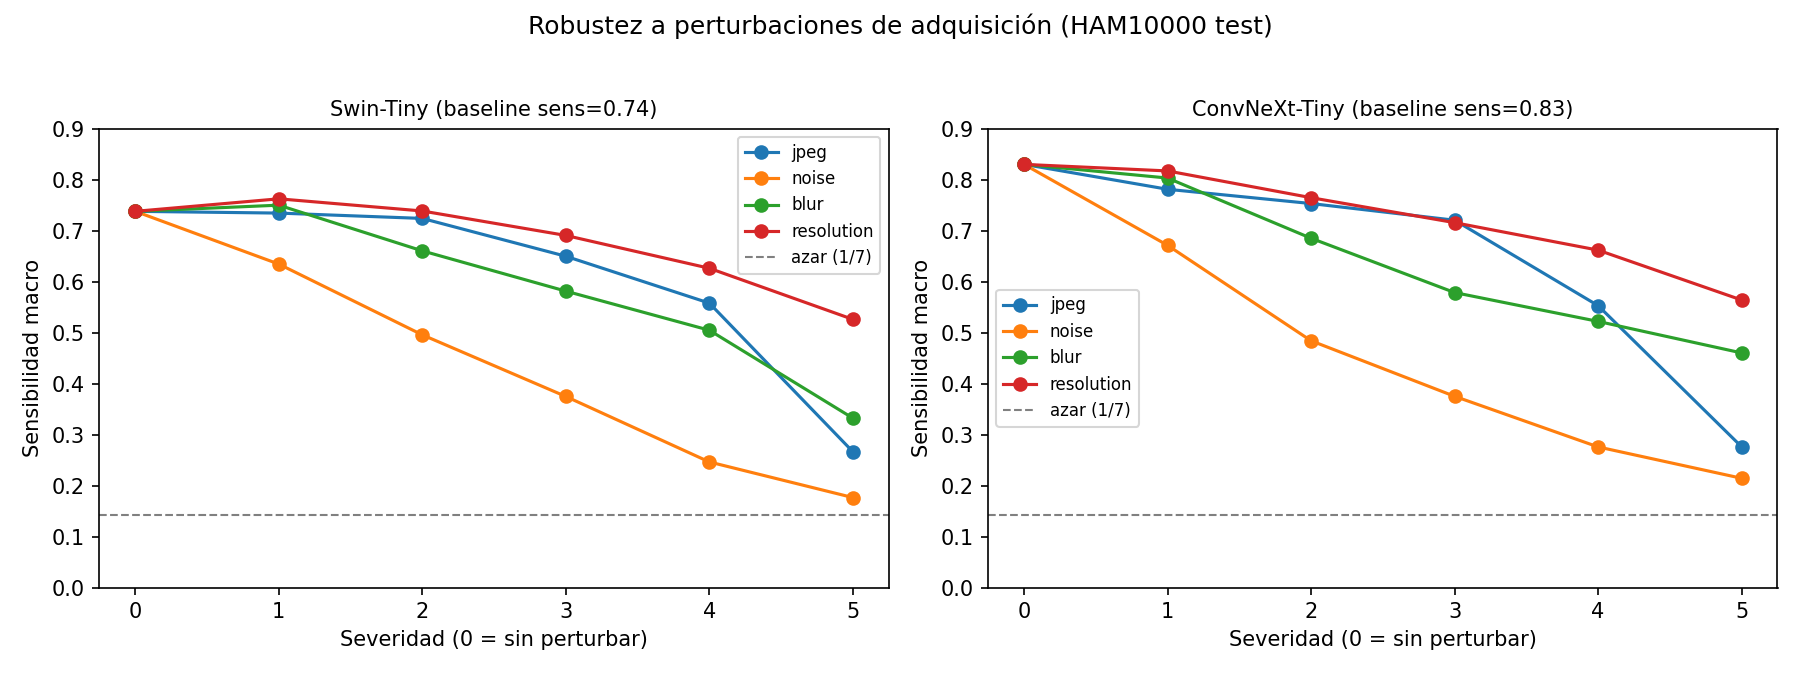
\includegraphics[width=\textwidth]{P24_robustness.png}
  \caption{Sensibilidad macro vs.\ severidad de perturbación (HAM10000 test). El ruido degrada más rápido;
  la resolución es la perturbación mejor tolerada. Línea punteada = azar ($1/7$).}
  \label{fig:robustez}
\end{figure}

Para hacer tangible el efecto, la Figura~\ref{fig:robustez_ej} muestra \emph{dos ejemplos} sometidos a
las cuatro perturbaciones en sus cinco niveles, con la predicción de Swin en cada caso: se aprecia cómo la
imagen se degrada y en qué punto la predicción pasa de correcta (verde) a incorrecta (rojo) —en ambos
casos el ruido y el JPEG severo son los que antes hacen fallar al modelo, coherente con las curvas
agregadas de la Figura~\ref{fig:robustez}—.

\begin{figure}[htbp]
  \centering
  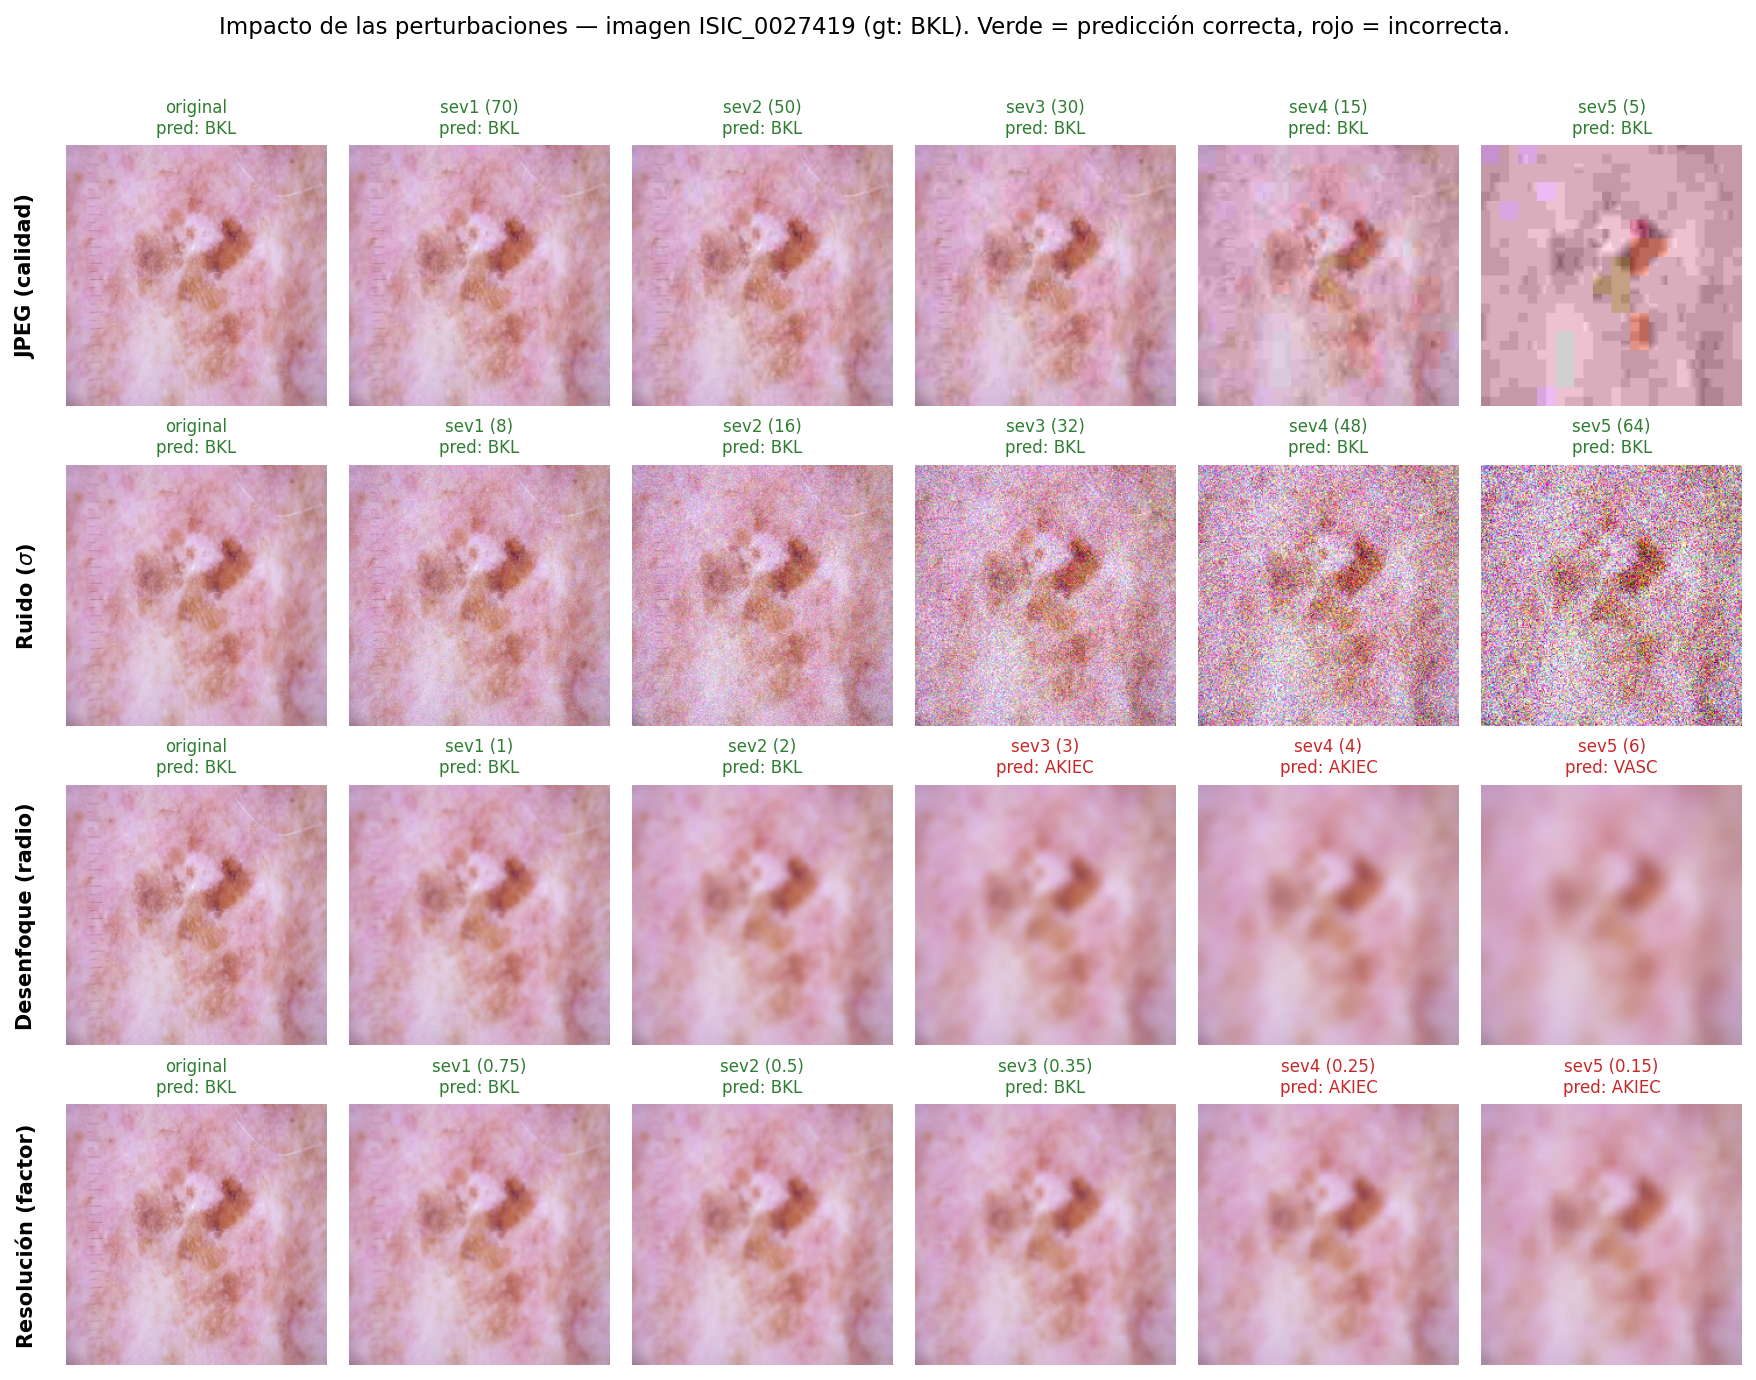
\includegraphics[width=\textwidth]{P24_robustness_examples.png}
  \caption{Impacto de cada perturbación sobre dos imágenes de test (dos casos de benign keratosis),
  elegidas por reflejar la tendencia agregada de la Figura~\ref{fig:robustez}. Filas: las cuatro
  perturbaciones; columnas: imagen original y severidades sev1--sev5 (entre paréntesis, el
  valor del parámetro). El título de cada panel indica la predicción de Swin-Tiny, en \textbf{verde} si
  coincide con el \emph{ground truth} y en \textbf{rojo} si no. En los dos casos, el ruido vuelca la
  predicción primero (sev1--sev3) y el JPEG severo también falla, mientras que desenfoque y resolución se
  toleran mucho mejor (fallan recién en sev5 o directamente no fallan).}
  \label{fig:robustez_ej}
\end{figure}

\subsection{Interpretabilidad: ¿el modelo mira la lesión?}
\label{sec:interpret}
Además de resistir degradaciones de imagen, conviene verificar que el modelo atiende información
clínicamente relevante y no artefactos incidentales de la fotografía. Un modelo puede acertar por la razón equivocada —fijándose en el fondo, en una regla milimétrica o en un
marcador de tinta en lugar de la lesión—. Para explorarlo se calcularon \textbf{mapas de saliencia}, que
señalan qué píxeles influyeron más en la decisión. Conviene enmarcar esto correctamente: se trata de un
\textbf{análisis cualitativo complementario} de la atención espacial del modelo, \emph{no} de una prueba de
que su razonamiento sea clínicamente correcto —eso requeriría la evaluación de un especialista—. Se usaron dos técnicas complementarias
(Figura~\ref{fig:interpret}). \emph{Grad-CAM} sobre Swin-Tiny: retropropaga el gradiente de la clase
predicha hasta el último bloque convolucional y pondera cada canal de activación por ese gradiente,
produciendo un mapa de calor de baja resolución donde las zonas \textbf{cálidas (rojas)} son las que más
empujaron la predicción. \emph{Saliencia por gradiente} sobre DermLIP: como es un clasificador por
similitud imagen--texto, se retropropaga la similitud imagen--diagnóstico hasta los píxeles de entrada;
la magnitud del gradiente en cada píxel indica cuánto altera esa similitud. En ambos modelos las zonas
destacadas se concentran \textbf{sobre la lesión} —no sobre piel sana ni artefactos—, siendo los mapas de
Swin más focalizados y los de DermLIP más difusos, con un patrón de \textbf{rejilla/puntos periódico}
visible en varios casos (Figura~\ref{fig:interpret}) —probablemente un artefacto de la tokenización en
parches del \emph{Vision Transformer} subyacente (ViT-B/16), no una señal clínica—. Un caso ilustrativo: en un basocarcinoma, Swin atiende
la región correcta pero lo clasifica como melanoma —mira lo correcto y aun así confunde clases
visualmente similares: un error de \emph{discriminación}, no de atención—.

\begin{figure}[htbp]
  \centering
  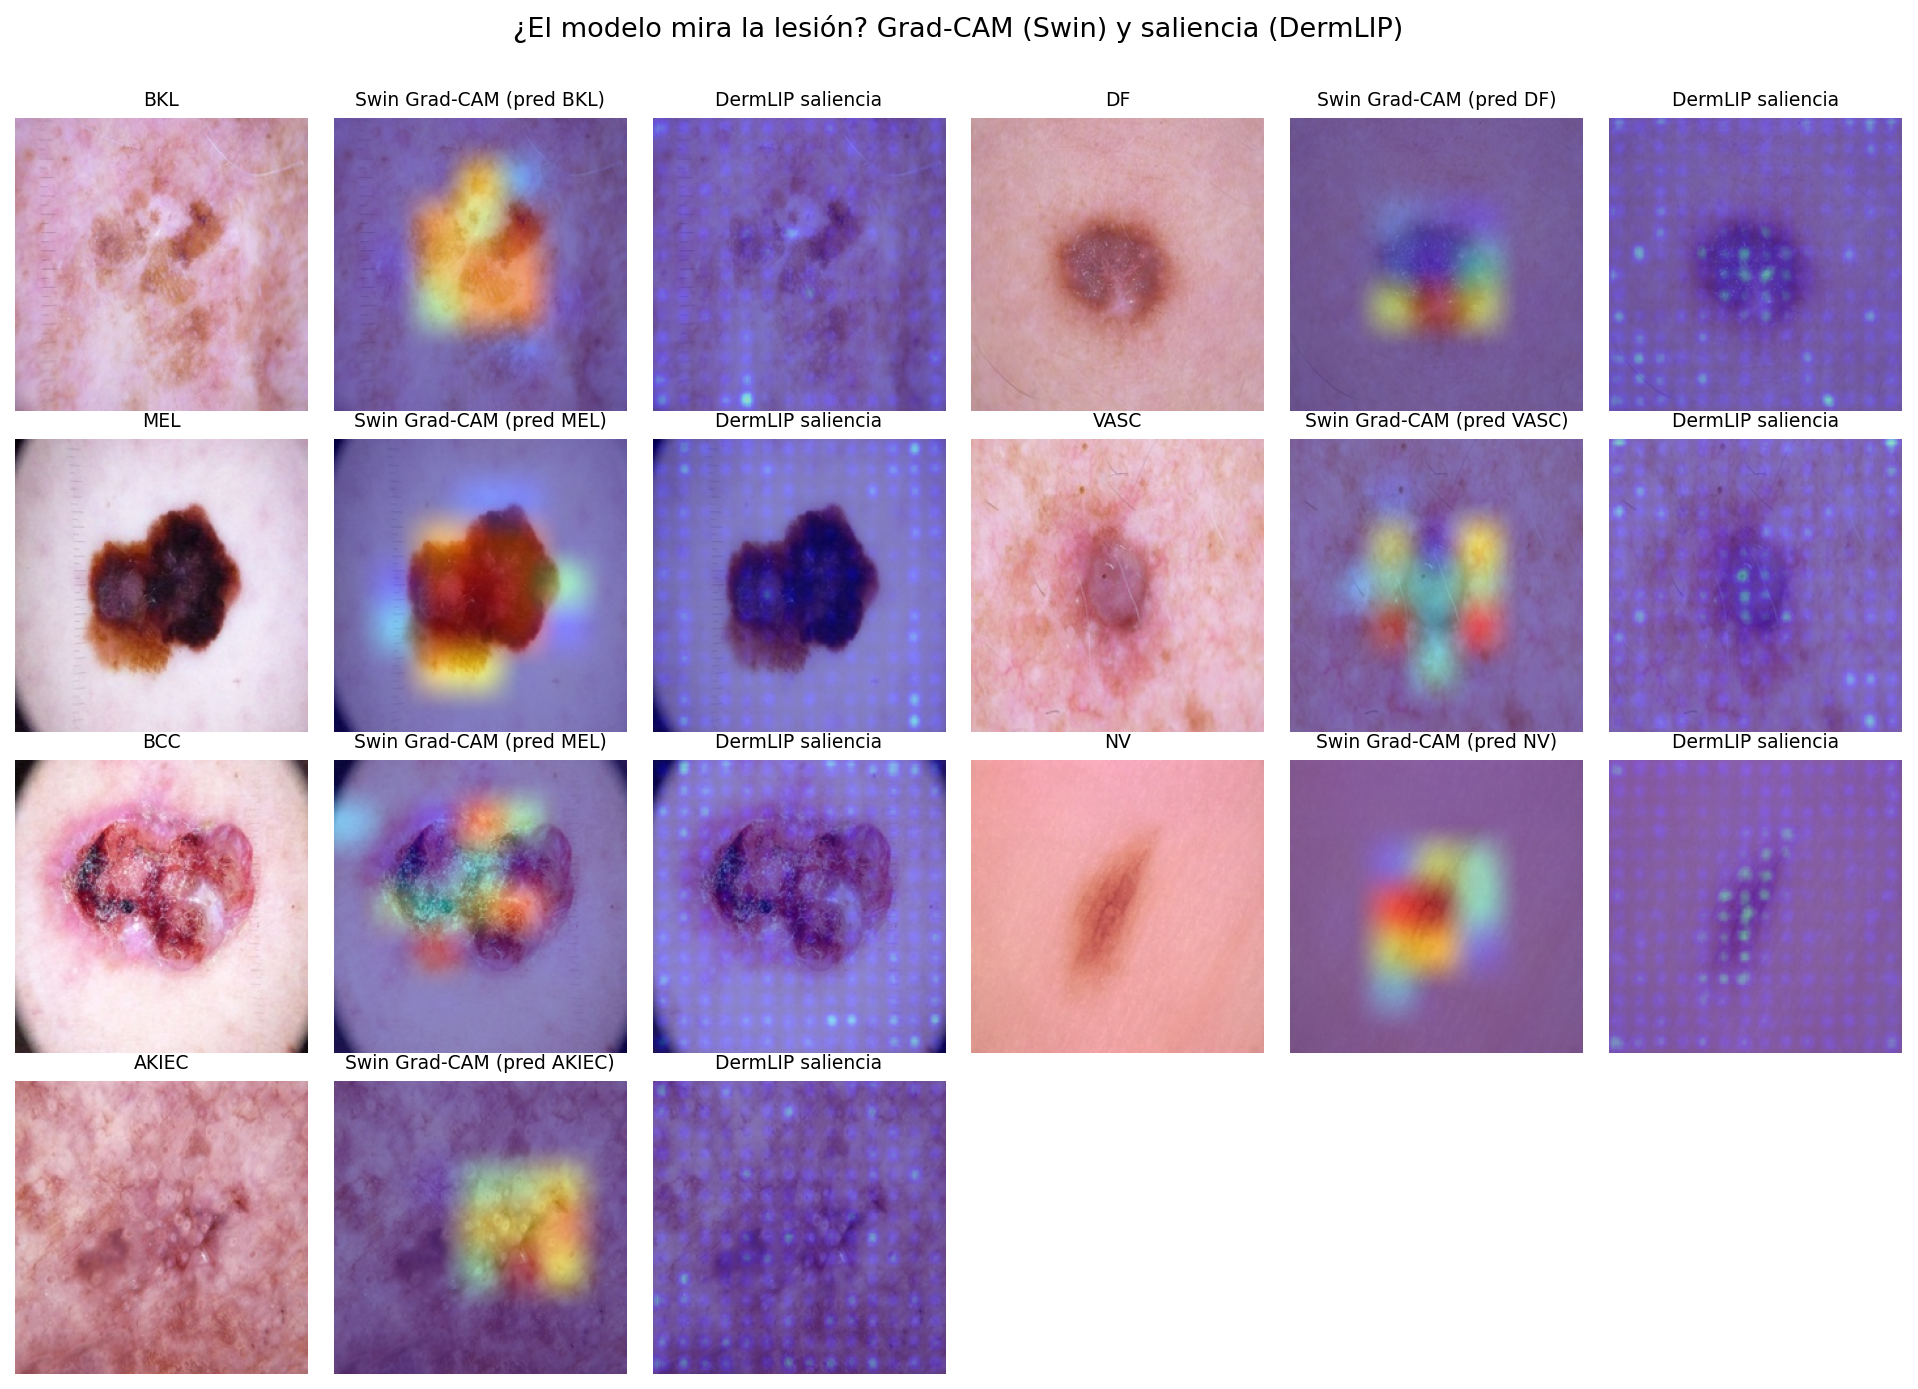
\includegraphics[width=\textwidth]{P25_interpretability.png}
  \caption{Mapas de saliencia, dos clases por fila; cada clase ocupa tres paneles: imagen original,
  Grad-CAM de Swin-Tiny (rojo = mayor contribución a la clase predicha) y saliencia por gradiente de
  DermLIP. En ambos modelos las zonas cálidas caen sobre la lesión y no sobre el fondo. Es evidencia
  cualitativa complementaria de que el modelo atiende la región relevante, no una prueba de validez
  clínica (que requeriría un especialista).}
  \label{fig:interpret}
\end{figure}

\subsection{Detección de melanoma: evaluación clínica binaria}
\label{sec:melanoma}
El caso del basocarcinoma que Swin confunde con melanoma (Sección~\ref{sec:interpret}) —mirando la región
correcta y aun así equivocándose— anticipa la pregunta de esta sección: dentro de la clasificación
multiclase, ¿qué tan bien se resuelve específicamente el caso más grave? Hasta aquí la evaluación fue
\emph{multiclase} (7 categorías), que es la formulación más exigente. Pero
un evaluador clínico se hace una pregunta más específica: \emph{¿qué tan bien detecta el sistema el
melanoma?} —la lesión cuyo diagnóstico tardío es más grave—. Esto conecta con un punto terminológico:
el título de la tesina habla de \emph{detección}, mientras que los resultados anteriores son de
\emph{clasificación}. No hay contradicción: la \emph{detección} en el sentido de \emph{localización}
(¿dónde está la lesión?) viene resuelta por el protocolo de adquisición —las imágenes de HAM10000 y HIBA
son dermatoscópicas \textbf{ya recortadas y centradas en una única lesión}, no hay múltiples lesiones que
localizar—, por lo que el trabajo se concentra en el diagnóstico; y la \emph{detección de melanoma} en el
sentido de \emph{cribado} (¿es melanoma o no?) se operacionaliza precisamente como la \textbf{clasificación
binaria melanoma-vs-resto} que se reporta a continuación. En ese sentido, el binario \emph{es} la detección
de melanoma.

Además de los clasificadores individuales se evalúa un \textbf{ensamble por voto suave} (promedio de las
probabilidades de Swin-Tiny y ConvNeXt-Tiny, ambos con TTA). Conviene situar su aporte: en la tarea
\emph{multiclase} de 7 clases su ganancia es \textbf{modesta} —sensibilidad macro $0.846$ frente a $0.827$
del mejor individual (ConvNeXt-Tiny), es decir $+0.019$, y $+0.004$ en F1 ponderado— a costa de
\textbf{duplicar} el tiempo de inferencia por usar dos modelos.\footnote{Medido con los checkpoints
\emph{modern\_v3} locales y TTA para que la comparación ensamble-vs-individual sea bajo el mismo protocolo;
por eso estos valores no coinciden con los \emph{headline} del Cuadro~\ref{tab:clasificacion}, obtenidos
con el checkpoint del barrido.} Para el problema \emph{in-distribution} ya casi saturado, apilar modelos
resulta una palanca más cara que el TTA sobre un único modelo especializado. En la detección binaria de
melanoma, en cambio, ese mismo ensamble sí aporta el mejor AUC-ROC, como se ve a continuación.

Se evaluaron dos tareas binarias sobre las probabilidades del clasificador (con TTA): \textbf{melanoma-vs-resto}
(score $=P(\text{MEL})$) y \textbf{maligno-vs-benigno} (maligno $=$ \{MEL, BCC, AKIEC\}). Se reporta la suite
clínica estándar: AUC-ROC, PR-AUC, sensibilidad, especificidad y valor predictivo negativo (VPN)
(Cuadro~\ref{tab:melanoma}), junto con la \textbf{tasa de falsos negativos (FN) de melanoma}, que es el
complemento de la sensibilidad en el punto de operación y por eso se discute en el texto en lugar de
tabularse. El punto de operación de las
variantes optimizadas se fija en el \emph{split de validación} y se aplica al test (sin sesgo optimista).

\begin{table}[H]
  \centering
  \caption{Detección de melanoma sobre HAM10000 test ($n=1503$), en dos tareas binarias (las filas en
  cursiva son encabezados de bloque, no datos). AUC-ROC y PR-AUC son independientes del umbral;
  ``esp$\ge$85'' fija el punto de operación en validación exigiendo especificidad $\ge0.85$ (prioriza no
  perder melanomas); Espec.\ y VPN son los valores efectivamente alcanzados en test bajo ese punto de
  operación. La tasa de falsos negativos es el complemento de Sens.\ (esp$\ge$85), por lo que no se tabula
  aparte. ``---'' = no disponible.}
  \label{tab:melanoma}
  \small
  \resizebox{\textwidth}{!}{%
  \begin{tabular}{lcccccc}
    \toprule
    \textbf{Modelo} & \textbf{AUC-ROC} & \textbf{PR-AUC} & \textbf{Sens.\ (argmax)} & \textbf{Sens.\ (esp$\ge$85)} & \textbf{Espec.} & \textbf{VPN} \\
    \midrule
    \multicolumn{7}{@{}l}{\itshape Tarea A --- Melanoma-vs-resto (prevalencia $0.11$)} \\
    Swin-Tiny        & 0.931 & 0.705 & 0.731 & 0.862 & 0.858 & 0.980 \\
    ConvNeXt-Tiny    & 0.949 & \textbf{0.811} & 0.731 & 0.910 & \textbf{0.862} & 0.987 \\
    Ensamble (voto)  & \textbf{0.954} & 0.799 & \textbf{0.760} & \textbf{0.928} & 0.860$^{\ast}$ & \textbf{0.990} \\
    \midrule
    \multicolumn{7}{@{}l}{\itshape Tarea B --- Maligno-vs-benigno (prevalencia $0.20$)} \\
    Swin-Tiny        & 0.936 & 0.823 & --- & 0.857 & $\ge0.85$ & --- \\
    ConvNeXt-Tiny    & 0.959 & \textbf{0.898} & --- & \textbf{0.942} & $\ge0.85$ & --- \\
    Ensamble (voto)  & \textbf{0.961} & 0.891 & --- & 0.922 & $\ge0.85$ & --- \\
    \bottomrule
  \end{tabular}%
  }
  \\[2pt]
  {\footnotesize $^{\ast}$El punto de operación del ensamble se fija sobre su propio score (voto), por lo
  que la especificidad efectiva puede diferir levemente de la de los modelos individuales aun exigiendo el
  mismo $\ge0.85$ en validación. Espec.\ y VPN de maligno-vs-benigno no se registraron por modelo más allá
  de la restricción de diseño ($\ge0.85$); Sens.\ (argmax) tampoco se calculó para esa tarea.}
\end{table}

Tres lecturas: (i) la capacidad de \emph{discriminación} de melanoma es \textbf{alta} —AUC-ROC
$0.93$--$0.95$ y macro-AUC one-vs-rest $0.94$--$0.96$—, mayor de lo que sugerían la exactitud o el F1
(el AUC no depende del umbral); (ii) el \textbf{argmax por defecto es clínicamente peligroso}: pierde el
$\approx$27\% de los melanomas (tasa de FN $0.27$), efecto de optimizar la exactitud global sobre un
problema desbalanceado; (iii) \textbf{optimizar el punto de operación} —tolerando más falsos positivos para
no perder melanomas— baja la tasa de FN a $\mathbf{0.07}$--$0.14$ (hasta $0.072$ en el ensamble;
$0.07$--$0.09$ en los mejores modelos, ConvNeXt y el ensamble) con VPN $\approx0.99$, un punto de
operación que prioriza el error clínicamente más costoso. Todo esto con clasificadores \emph{Tiny} ($\sim$28\,M de parámetros) en GPU de
consumo, en línea con el eje de hardware accesible de la tesina (Sección~\ref{sec:intro}).

El Cuadro~\ref{tab:sota_melanoma} sitúa el AUC-ROC de melanoma-vs-resto frente a la literatura de detección
binaria: el ensamble ($0.954$) queda a la par de la referencia SOTA más citada para esta tarea
(Kreouzi~\cite{Kreouzi2024}, DenseNet121 sobre DermNet, AUC $0.951$), lograda con una fracción del cómputo
(clasificadores \emph{Tiny} vs.\ un modelo de propósito específico). La comparación es \textbf{orientativa}:
los protocolos y datasets difieren (HAM10000 vs.\ DermNet/ISIC), y el trabajo de Kreouzi no reporta AUC para
su variante de mayor exactitud (ensamble de tres redes, $97.67\%$ Acc. sobre ISIC, no comparable
directamente con el AUC de este trabajo).

\begin{table}[htbp]
  \centering
  \caption{Detección de melanoma vs.\ estado del arte (tarea binaria melanoma-vs-resto). Este trabajo:
  HAM10000 test ($n=1503$), umbral fijado en validación (esp.\ objetivo $\ge0.85$). Las referencias del
  SOTA se evalúan sobre datasets distintos (DermNet/ISIC) y en binario puro, por lo que la comparación es
  \textbf{orientativa}. Mejor de este trabajo en negrita.}
  \label{tab:sota_melanoma}
  \resizebox{\textwidth}{!}{%
  \begin{tabular}{llcrrr}
    \toprule
    \textbf{Referencia} & \textbf{Modelo} & \textbf{Dataset} & \textbf{AUC-ROC} & \textbf{Sens.\ (\%)} & \textbf{Acc.\ (\%)} \\
    \midrule
    \multicolumn{6}{@{}l}{\itshape Estado del arte} \\
    \cite{Kreouzi2024} & DenseNet121 & DermNet & 0.951 & --- & 92.30 \\
    \cite{Kreouzi2024} & DenseNet121$+$ResNet50$+$EffNetB3 (ens.) & ISIC & --- & --- & 97.67 \\
    \midrule
    \multicolumn{6}{@{}l}{\itshape Este trabajo (HAM10000, umbral fijado en validación)} \\
    & Swin-Tiny ($\sim$28\,M)      & HAM10000 & 0.931 & 86.2 & --- \\
    & ConvNeXt-Tiny ($\sim$28\,M)  & HAM10000 & 0.949 & 91.0 & --- \\
    & Ensamble (Swin$+$ConvNeXt)   & HAM10000 & \textbf{0.954} & \textbf{92.8} & --- \\
    \bottomrule
  \end{tabular}%
  }
\end{table}

\paragraph{Conclusión parcial (clasificación).} Para clasificar lesiones conviene un modelo
\emph{especializado}: un CNN/ViT supervisado (mejor exactitud) o un VL classifier derm-específico
(fuerte incluso sin entrenamiento sobre el dataset objetivo). Los VLMs generativos generales no son
competitivos en esta tarea, hecho que la literatura también constata (Sección~\ref{sec:rediag}). Y, para
el problema clínicamente crítico —la detección de melanoma— un clasificador chico bien calibrado en su
punto de operación alcanza sensibilidad $\approx0.93$ con tasa de FN $\approx0.07$ (Sección~\ref{sec:melanoma}).

% ============================================================
\section{Generación de reportes}
\label{sec:gen}
% ============================================================
La segunda parte de la tesina evalúa si un VLM puede \emph{describir} la lesión en un reporte clínico.
Antes de los resultados, conviene ver la \emph{forma} de los reportes generados. La
Figura~\ref{fig:estructura} muestra un ejemplo típico: el modelo describe rasgos morfológicos (color,
forma, bordes, superficie, localización) y —en el mejor caso— concluye con un diagnóstico.\footnote{Los
reportes generados se muestran en su idioma original (inglés), tal como los produce el modelo.}

\begin{figure}[H]
\centering
\fbox{\parbox{0.96\textwidth}{\footnotesize
\begin{minipage}[c]{0.24\textwidth}
  \centering
  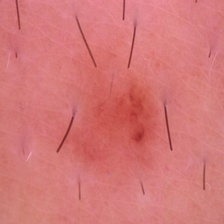
\includegraphics[width=\textwidth]{ej_ISIC_0024321.jpg}\\[2pt]
  {\scriptsize ISIC\_0024321\\ \emph{gt}: nevo}
\end{minipage}\hfill
\begin{minipage}[c]{0.70\textwidth}\itshape
``The diagnosis is a nevus, a benign pigmented lesion. Key features: (1) color brownish-red to
reddish-brown; (2) shape irregular, asymmetrical, with a lobulated border; (3) surface rough and
slightly elevated; (4) located on the lower leg, a common site for nevi. The absence of rapid growth or
ulceration helps rule out malignancy.''
\end{minipage}
}}
\caption{Ejemplo de la estructura típica de un reporte generado sobre una imagen de nevo: descripción
morfológica seguida de una conclusión diagnóstica.}
\label{fig:estructura}
\end{figure}

\subsection{Diseño del experimento y resultados directos}
\label{sec:gen_diseno}
\paragraph{Ajuste en dos etapas.} El VLM generador se entrenó en dos etapas: \emph{(1) alineamiento
visual--textual}, ajustando la proyección entre el codificador visual y el modelo de lenguaje con las
descripciones de SkinCAP; y \emph{(2) ajuste de instrucciones} con LoRA, usando las narrativas de
SkinCoT para que el modelo aprenda a producir un reporte a partir de la imagen. Se entrena con SkinCaRe
(foto clínica, que \emph{sí} trae texto asociado) porque HAM \emph{no} tiene reportes de referencia,
solo etiquetas.

\paragraph{Cómo se evalúa.} Una vez entrenado, el modelo \emph{genera} reportes para imágenes de prueba.
Se emplean los dos niveles de evaluación definidos en la Sección~\ref{sec:metricas}: el \textbf{Nivel 2}
mide la \emph{fidelidad clínica} sin necesidad de un reporte de referencia —\emph{diagnostic consistency}
(¿el reporte nombra el diagnóstico correcto?) y \emph{clinical entity recall} (¿menciona las entidades
clínicas esperadas?)—, mientras que el \textbf{Nivel 1} mide la \emph{calidad textual} comparando contra
un reporte de referencia (BLEU/ROUGE/METEOR de solapamiento y BERTScore de similitud semántica).
\emph{En HAM} la evaluación es de \emph{Nivel 2}, justamente porque HAM no tiene reportes de referencia
pero sí etiquetas diagnósticas con las que verificar la fidelidad. \emph{En SkinCoT}
(Sección~\ref{sec:skincot}) la evaluación es de \emph{Nivel 1} (con referencia). Esta separación explica por qué se \emph{entrena} con SkinCoT pero se
\emph{evalúa la fidelidad} sobre HAM: cada dataset aporta lo que el otro no tiene.

\paragraph{Resultado directo.} El Cuadro~\ref{tab:generacion_v1v2} compara dos iteraciones del ajuste de
la segunda etapa. La diferencia entre ellas es la \emph{duración del entrenamiento}: la v1 usó 3 épocas
y la v2, 10 épocas (con los mismos hiperparámetros del mejor punto del barrido), buscando mejorar la
convergencia; además, la v2 incorporó una instrucción de generación corregida. De v1 a v2, el
\emph{recall} de entidades sube (reportes más ricos) pero la \emph{diagnostic consistency}
\textbf{empeora}: el modelo describe mejor, pero acierta menos el diagnóstico —es decir, más
entrenamiento no resolvió el problema, lo que orientó el análisis hacia su verdadera causa.

\begin{table}[H]
  \centering
  \caption{Generación de reportes en HAM10000 (Nivel 2), \emph{sobre el texto completo}. El ajuste v2
  enriquece los reportes pero la consistencia diagnóstica empeora. \emph{Nota:} estos valores se computan
  sobre el texto completo (antes de la corrección de la Sección~\ref{sec:reprazon}), por lo que la
  consistencia está \emph{sobreestimada} respecto de los cuadros posteriores, que se miden solo sobre el
  reporte; por eso el baseline aquí (LLaVA $0.634$, Mini $0.229$) difiere del de la
  Sección~\ref{sec:res_ensamble}, medido sobre el reporte y con otro \emph{prompt}.}
  \label{tab:generacion_v1v2}
  \begin{tabular}{lcccc}
    \toprule
    \textbf{Modelo} & \multicolumn{2}{c}{\textbf{Diagnostic consistency}} & \multicolumn{2}{c}{\textbf{Clinical entity recall}} \\
    & v1 & v2 & v1 & v2 \\
    \midrule
    LLaVA-Med & \textbf{0.718} & 0.634 & 0.457 & \textbf{0.824} \\
    Mini-VLM  & \textbf{0.353} & 0.229 & \textbf{0.607} & 0.546 \\
    \bottomrule
  \end{tabular}
\end{table}

La causa, como se analiza a continuación, es que el modelo enumera diagnósticos diferenciales sin
\emph{comprometerse} con uno. A este comportamiento lo llamamos \textbf{\emph{hedging}}: el reporte
``se cubre'' en lugar de concluir.

\subsection{Hallazgo metodológico: reporte vs.\ razonamiento}
\label{sec:reprazon}
\paragraph{Por qué surge la diferencia.} El conjunto de la segunda etapa es SkinCoT, cuyo nombre
proviene de \emph{Chain-of-Thought}: sus textos de referencia \emph{son}, deliberadamente, narrativas de
razonamiento diagnóstico paso a paso, no reportes concluyentes. En ellos, los pasos de razonamiento se
delimitan con bloques \texttt{<think>\dots</think>}. Al entrenar con esos textos completos, el modelo
\emph{aprende a reproducir el razonamiento} —incluidos esos bloques—, mezclando ``razonamiento'' y
``reporte'' en una sola salida.

\paragraph{El razonamiento no es solo un problema.} Conviene matizar: los bloques \texttt{<think>} tienen
valor —permiten \emph{auditar el proceso} por el que el modelo llega a un diagnóstico, lo que es
deseable para la interpretabilidad clínica—. El problema no es que el modelo razone, sino que (a) el
razonamiento se \emph{mezcla} con el reporte, y (b) ese razonamiento es donde ocurre el \emph{hedging}.

\paragraph{Por qué importa para la evaluación.} La \emph{diagnostic consistency} busca el diagnóstico
correcto en el texto. Si se evalúa el texto \emph{completo}, las menciones que el modelo hace
\emph{dentro} de su razonamiento (donde hipotetiza varias clases) cuentan como aciertos, lo que
\textbf{infla} la métrica. Lo medimos sobre los mismos reportes (LLaVA-Med, condición controlada),
comparándolos con y sin los bloques \texttt{<think>}: la consistencia pasó de $0.60$ sobre el texto
completo a $0.30$ al evaluar únicamente el \emph{reporte}. Casi la mitad de la ``fidelidad'' provenía del
razonamiento. Por ello, en adelante todas las métricas de
generación se computan \textbf{sobre el reporte}, separándolo del razonamiento.

\subsection{Por qué un ensamble en cascada}
\label{sec:porque_ensamble}
A esta altura hay \emph{dos problemas independientes}: (i) los VLMs no clasifican bien
(Sección~\ref{sec:clasif}); y (ii) cuando generan, no se comprometen con un diagnóstico. La estrategia
propuesta es un \textbf{ensamble en cascada} (Figura~\ref{fig:cascada}) que \emph{desacopla} las tareas:
un \textbf{clasificador especializado} decide el diagnóstico, y un \textbf{VLM generativo} redacta el
reporte \emph{condicionado} a ese diagnóstico. A inyectar el diagnóstico del clasificador en la
instrucción del generador lo llamamos \textbf{\emph{grounding}} (anclaje).

\begin{figure}[H]
\centering
\begin{tikzpicture}[
  box/.style={rectangle, rounded corners, draw, thick, align=center, minimum height=1.1cm, font=\small},
  >=Stealth, node distance=0.85cm]
  \node[box] (img) {Imagen};
  \node[box, draw=vlcls, right=of img] (clf) {Clasificador\\ (Swin / DermLIP)};
  \node[box, fill=gray!8, right=of clf] (dx) {diagnóstico\\ predicho};
  \node[box, draw=vlmgen, right=of dx] (gen) {VLM generativo\\ (\emph{grounded, noreasoning})};
  \node[box, right=of gen] (rep) {Reporte\\ comprometido};
  \draw[->] (img)--(clf); \draw[->] (clf)--(dx); \draw[->] (dx)--(gen);
  \draw[->] (img.south) to[bend right=20] (gen.south);
  \draw[->] (gen)--(rep);
\end{tikzpicture}
\caption{Ensamble en cascada: el clasificador aporta el diagnóstico, que se inyecta (junto con la
imagen) en el \emph{prompt} del generador; este produce un reporte que afirma ese diagnóstico.
\emph{Noreasoning}: variante de \emph{prompt} que prohíbe explícitamente razonar antes de concluir
(se justifica en el párrafo siguiente).}
\label{fig:cascada}
\end{figure}

\paragraph{Cómo funciona y por qué ayuda.} El clasificador (que \emph{sí} discrimina) entrega un
diagnóstico; el generador lo recibe en el \emph{prompt} y produce un reporte que debe afirmarlo. Esto
ataca directamente las dos fallas: el diagnóstico ya no depende del juicio colapsado del VLM, y el
generador tiene un diagnóstico concreto al que comprometerse en lugar de \emph{hedear}. Además es modular (no
requiere re-entrenar ni fusionar modelos) y de bajo costo.

\paragraph{Limitaciones del enfoque.} El ensamble no es gratis: (a) \emph{hereda los errores del
clasificador} —si este se equivoca, el reporte se compromete con un diagnóstico incorrecto
(Sección~\ref{sec:res_ensamble})—; (b) usa \emph{dos modelos} en lugar de uno, con mayor costo de
cómputo y orquestación; y (c) no es un sistema \emph{end-to-end}. Frente a alternativas: un VLM
\emph{más grande} podría, en principio, clasificar y generar a la vez, pero los VLMs grandes generales
mostraron la misma limitación de discriminación (Sección~\ref{sec:clasif_sota}), por lo que ``más
parámetros'' no resuelve por sí solo el problema; y un modelo \emph{supervisado} clasifica mejor pero no
genera texto. El ensamble es un punto intermedio pragmático: combina lo mejor de cada familia sin
entrenar un modelo nuevo.

\paragraph{El \emph{grounding} debe forzar el compromiso: la variante \emph{noreasoning}.} Inyectar el
diagnóstico no basta: por su prior de razonamiento, el modelo tiende a ``pensar en voz alta'' y a veces
a contradecir el diagnóstico provisto. Se iteró el \emph{prompt} (usando el diagnóstico correcto, para
aislar el mecanismo) midiendo la consistencia \emph{sobre el reporte} (LLaVA-Med, \emph{grounding} oracle):
un \emph{prompt} suave logró $0.30$; uno que prohíbe enumerar diferenciales, $0.70$; y la variante
\textbf{\emph{noreasoning}} —que prohíbe explícitamente producir razonamiento o bloques \texttt{<think>} y
exige solo el reporte final— alcanzó $0.85$. Esta es la variante adoptada; son mediciones de \emph{ajuste
de prompt} sobre el oracle, no comparables directamente con las cifras de los cuadros de ensamble.

\subsection{Resultados del ensamble}
\label{sec:res_ensamble}
\paragraph{Condiciones comparadas.} Para medir el aporte del \emph{grounding} se comparan cuatro
condiciones, todas con el mismo generador y el \emph{prompt} \emph{noreasoning}:
\begin{itemize}[leftmargin=1.6em]
  \item \textbf{Baseline}: el generador \emph{sin grounding} (instrucción genérica ``describe esta
  lesión''). Es el punto de referencia o ``piso''.
  \item \textbf{Oracle}: \emph{grounding} con la etiqueta verdadera (\emph{ground truth}, \emph{gt}) de
  la imagen, es decir, el diagnóstico \emph{correcto}. No es un sistema usable en un entorno real (allí
  no se conoce la etiqueta de antemano); es un experimento de control que da la \emph{cota superior} del
  \emph{grounding}, aislando su efecto de los errores del clasificador.
  \item \textbf{Swin} y \textbf{DermLIP}: \emph{grounding} con la predicción de un clasificador
  \emph{real} (imperfecto). Representan el ensamble efectivamente utilizable; su distancia respecto al
  oracle es el costo de los errores de clasificación.
\end{itemize}
(\emph{gt} = \emph{ground truth}, la etiqueta diagnóstica real de la imagen.)

El Cuadro~\ref{tab:ensamble} y la Figura~\ref{fig:f2} muestran los resultados. La
Figura~\ref{fig:f2}(a) grafica la \emph{diagnostic consistency} y la (b) el \emph{recall}, por condición
(eje horizontal) y modelo (barras de color). Se observa:
\begin{enumerate}[leftmargin=1.6em]
  \item \textbf{El \emph{grounding} mejora drásticamente la fidelidad}, sobre todo en Mini-VLM
  ($0.246 \rightarrow 0.812$ con Swin), sin sacrificar la riqueza (el \emph{clinical entity recall} se
  mantiene $\approx 0.77$; como este cuadro tabula solo la consistencia, ese valor se reporta en los
  Cuadros~\ref{tab:rag} y \ref{tab:plantilla}).
  \item \textbf{La fidelidad crece con la calidad del clasificador}: un clasificador más exacto produce
  reportes más fieles (oracle $>$ Swin en ambos modelos, en consonancia con su exactitud 1.00 y 0.80). La
  progresión es \emph{monótona} en Mini-VLM (baseline $<$ DermLIP $<$ Swin $<$ oracle); en LLaVA-Med, en
  cambio, un clasificador \emph{débil} (DermLIP, 0.38) cae \emph{por debajo} de su propio baseline —lo que
  anticipa el punto siguiente—.
  \item \textbf{Un clasificador débil puede empeorar}: con DermLIP zero-shot (exactitud 0.38), LLaVA
  baja a $0.454$, por debajo de su baseline ($0.645$), porque el reporte se compromete con el
  diagnóstico \emph{equivocado}. Esto cuantifica el costo de propagación de error.
  \item \textbf{El techo del \emph{grounding} depende del generador}: con el diagnóstico \emph{correcto}
  inyectado, Mini-VLM lo enuncia casi siempre ($0.999$) pero LLaVA-Med se queda en $0.852$, es decir,
  \emph{omite el diagnóstico que se le dio} en uno de cada siete reportes. La causa es el prior de
  razonamiento del modelo más grande, ya cuantificado en la Sección~\ref{sec:porque_ensamble}: sobre
  LLaVA-Med con oracle, el ajuste de \emph{prompt} llevó la consistencia de $0.30$ (prompt suave) a $0.85$
  con la variante \emph{noreasoning}, y ese $0.85$ es exactamente el valor que reaparece aquí. Dicho de
  otro modo, $0.852$ no es una limitación del \emph{grounding} sino \textbf{el techo alcanzable por
  ingeniería de prompt} en un modelo que tiende a deliberar: incluso prohibiéndole razonar y dándole la
  respuesta, a veces divaga hacia diferenciales en lugar de comprometerse. Mini-VLM, más escueto y literal,
  se limita a transcribir el diagnóstico recibido, lo que explica su techo casi perfecto.
\end{enumerate}

Estas diferencias son \textbf{estadísticamente significativas}: un \emph{bootstrap} pareado ($2000$
remuestreos, sobre las mismas $1503$ imágenes) sobre Mini-VLM da un salto de $\Delta=+0.567$
$[0.536,\,0.596]$ entre \emph{baseline} y \emph{grounding} con Swin, y una ventaja de $\Delta=+0.315$
$[0.285,\,0.343]$ de Swin sobre DermLIP; la brecha residual respecto del oracle es $\Delta=0.187$
$[0.168,\,0.207]$ (el costo de los errores de clasificación). Los tres intervalos de confianza del $95\%$
excluyen el cero.

\begin{table}[H]
  \centering
  \caption{Ensamble (clasificador $\rightarrow$ generador \emph{noreasoning}). \emph{Diagnostic
  consistency} (sobre el reporte) en HAM10000 por condición y modelo, sobre el \textbf{test split completo
  ($n=1503$)}. La columna ``Acc.\ clasif.'' es la exactitud del checkpoint de Swin efectivamente usado
  como ancla en el pipeline de generación ($0.80$, single-view), distinta del \emph{headline} con TTA
  ($0.868$, Cuadro~\ref{tab:clasificacion}).}
  \label{tab:ensamble}
  \begin{tabular}{llcc}
    \toprule
    \textbf{Grounding} & \textbf{Acc.\ clasif.} & \textbf{LLaVA-Med} & \textbf{Mini-VLM} \\
    \midrule
    Baseline (sin grounding) & ---  & 0.645 & 0.246 \\
    DermLIP (ZS)             & 0.38 & 0.454 & 0.497 \\
    Swin (supervisado)       & 0.80 & \textbf{0.696} & \textbf{0.812} \\
    \midrule
    \textit{Oracle (gt) --- cota superior} & \textit{1.00} & \textit{0.852} & \textit{0.999} \\
    \bottomrule
  \end{tabular}
\end{table}

\begin{figure}[H]
  \centering
  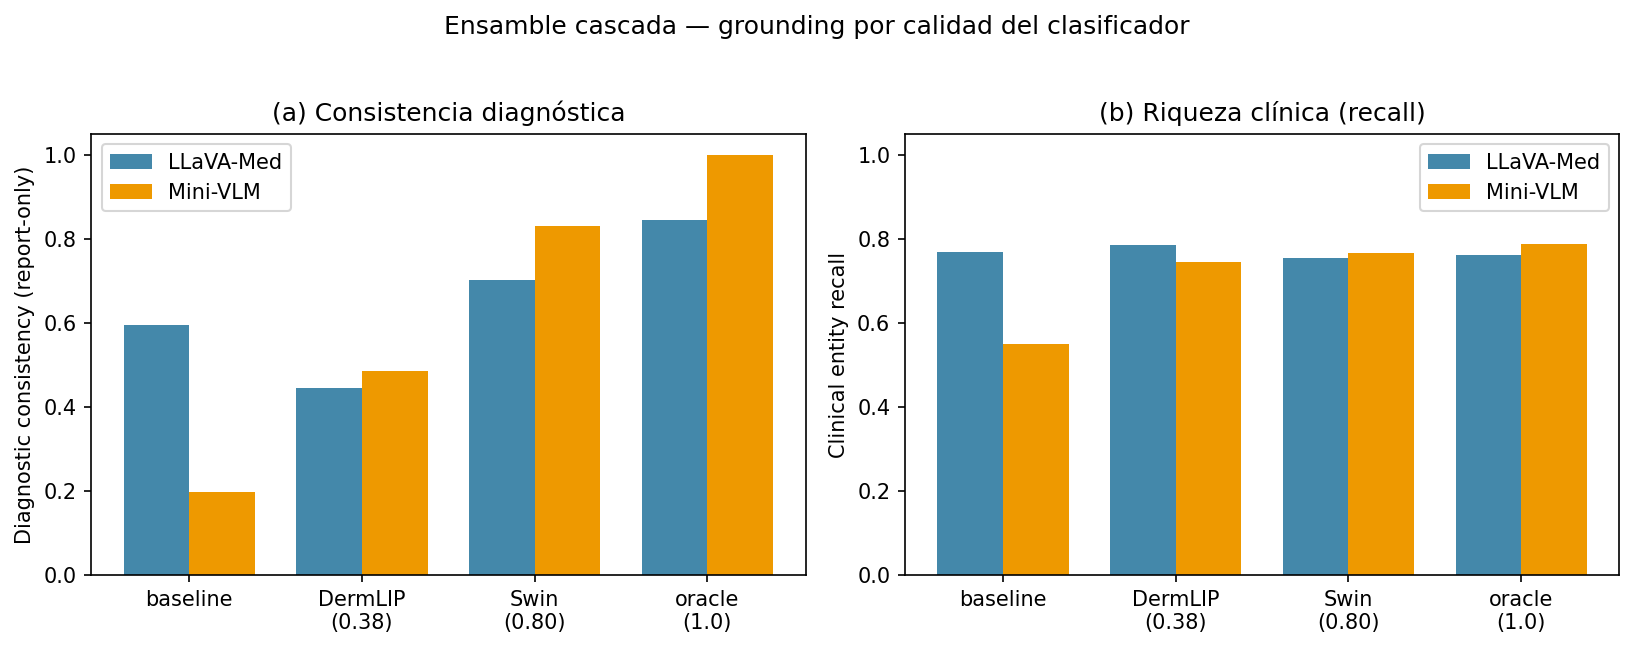
\includegraphics[width=\textwidth]{F2_ensamble.png}
  \caption{Ensamble cascada: (a) \emph{diagnostic consistency} (fidelidad) y (b) \emph{clinical entity
  recall} (riqueza), por condición de \emph{grounding} y modelo. La fidelidad crece con la calidad del
  clasificador; la riqueza se mantiene.}
  \label{fig:f2}
\end{figure}

\paragraph{Ejemplos.} La diferencia entre comprometerse y no hacerlo se ve claramente en el texto. El
\emph{baseline} \emph{hedea} (no concluye), mientras que con \emph{grounding} el mismo modelo afirma el
diagnóstico:

\begin{figure}[H]
\centering
\fbox{\parbox{0.96\textwidth}{\footnotesize
\begin{minipage}[c]{0.24\textwidth}
  \centering
  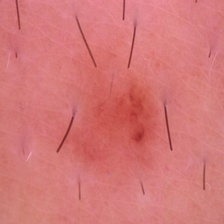
\includegraphics[width=\textwidth]{ej_ISIC_0024321.jpg}\\[2pt]
  {\scriptsize ISIC\_0024321\\ \emph{gt}: nevo}
\end{minipage}\hfill
\begin{minipage}[c]{0.70\textwidth}
\textbf{Sin grounding (baseline)} \textemdash\ \itshape ``To analyze the case I will follow a structured
approach\dots\ \textbf{1. High-Level Decision}: the category likely falls under \emph{inflammatory
conditions}\dots'' \upshape (razona, no concluye, y se desvía a una categoría incorrecta).\\[4pt]
\textbf{Con grounding (oracle, noreasoning)} \textemdash\ \itshape ``\textbf{The diagnosis is a nevus},
a benign pigmented lesion. Key features: color brownish-red, irregular lobulated border\dots'' \upshape
(afirma el diagnóstico y lo sustenta).
\end{minipage}
}}
\caption{Efecto del \emph{grounding}+\emph{noreasoning} sobre la misma imagen (un nevo, el mismo caso
ISIC\_0024321 de la Figura~\ref{fig:estructura}): de un reporte ambiguo a uno comprometido con el
diagnóstico correcto.}
\label{fig:ej_grounding}
\end{figure}

\subsection{Análisis por clase: ¿en qué clases ayuda el \emph{grounding}?}
\label{sec:porclase}
El promedio global oculta un comportamiento por clase muy informativo (Figura~\ref{fig:perclase}). El
\emph{grounding} ayuda \textbf{más en las clases minoritarias} donde el modelo sin anclaje casi nunca
nombraba el diagnóstico: en Mini-VLM, la consistencia de \emph{queratosis actínica} pasa de $0.00$ a
$0.83$, la de \emph{queratosis benigna} de $0.07$ a $0.77$ y la de \emph{carcinoma basocelular} de $0.08$
a $0.76$ (con el clasificador Swin). Mini-VLM se beneficia de forma casi uniforme —su \emph{baseline} era
muy pobre, había mucho margen—, mientras que LLaVA-Med, que ya tenía sesgo a nombrar melanoma y nevo,
gana sobre todo en las minoritarias. Un hallazgo clave es el reverso: un \textbf{clasificador débil
(DermLIP, $0.38$) daña justo las clases donde el generador ya era bueno} —en LLaVA-Med, melanoma cae de
$0.85$ a $0.69$ y nevo de $0.62$ a $0.43$— porque inyecta un diagnóstico equivocado que el modelo adopta.
Es la propagación de error, ahora resuelta clase por clase.

\begin{figure}[H]
  \centering
  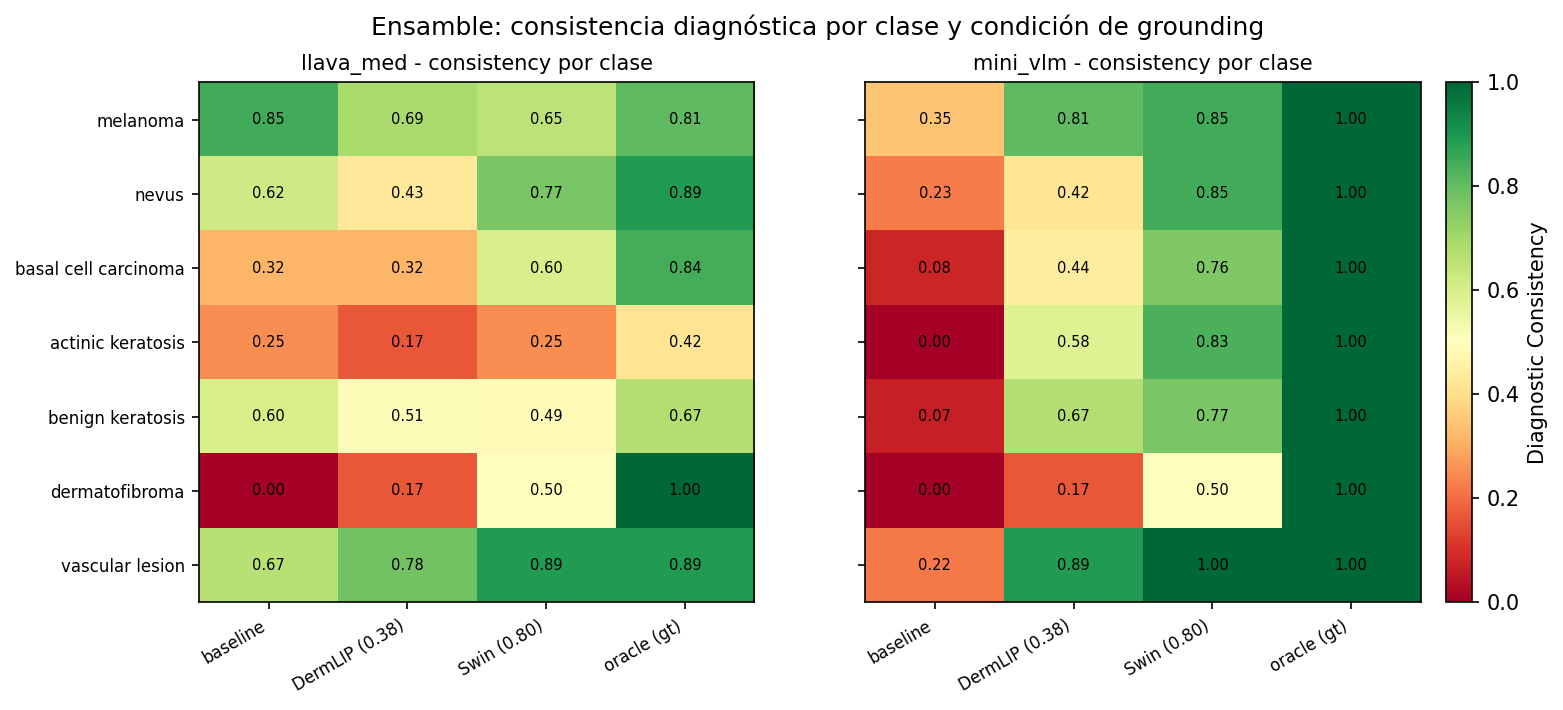
\includegraphics[width=\textwidth]{P03_perclass.png}
  \caption{Consistencia diagnóstica \emph{por clase} y condición de \emph{grounding} (verde alto, rojo
  bajo). El anclaje rescata sobre todo las clases minoritarias; un clasificador débil (DermLIP) puede
  degradar las clases que el generador ya nombraba bien.}
  \label{fig:perclase}
\end{figure}

\subsection{Taxonomía de errores}
\label{sec:taxonomia}
Para ir más allá de ejemplos aislados, se \emph{cuantificó} el análisis cualitativo: cada reporte
generado se clasificó automáticamente, con reglas determinísticas (búsqueda de menciones de clases y de
marcadores lingüísticos), en su \textbf{tipo de error principal}. Las categorías, con un ejemplo de cada
una, son:
\begin{itemize}[leftmargin=1.6em]
  \item \textbf{ok}: menciona el diagnóstico correcto y no dispara otras banderas. \emph{Ej.\ (gt
  melanoma):} ``\emph{Diagnosis --- Melanoma. Supporting features: irregularly shaped, pigmented nodules
  with a violaceous hue\ldots}''.
  \item \textbf{dx incorrecto} (\emph{dx} $=$ diagnóstico): no menciona el diagnóstico correcto pero sí
  \emph{otro}. \emph{Ej.\ (gt
  nevo):} ``\emph{Diagnosis: Dermatofibroma. Supporting features: a well-circumscribed brown nodule\ldots}''
  ---afirma con seguridad una clase equivocada---.
  \item \textbf{contradicción}: nombra \emph{dos o más} diagnósticos distintos en el mismo reporte.
  \emph{Ej.\ (gt nevo):} ``\emph{\ldots reveals homogeneous pigmentation with no signs of melanoma. The
  diagnosis is a benign nevus\ldots}'' ---nombra melanoma y nevo---.
  \item \textbf{hedging}: lenguaje de incertidumbre sin comprometerse (``\emph{could be\ldots}'',
  ``\emph{the category likely falls under inflammatory conditions\ldots}'').
  \item \textbf{repetición}: texto degenerado, con frases repetidas en bucle (p.ej.\ el reporte de la
  Figura~\ref{fig:ej_rep}, que repite ``\emph{\ldots irregular borders\ldots a hallmark of melanoma}'').
  \item \textbf{insuficiente}: reporte demasiado corto o sin contenido morfológico (una o dos frases
  genéricas, sin describir la lesión).
  \item \textbf{otros}: no encaja en las anteriores (p.ej.\ enuncia una enfermedad ajena a las 7 clases,
  como el ``tinea corporis'' de SkinVL).
\end{itemize}

\paragraph{No todos los errores pesan igual.} A efectos clínicos conviene distinguir su \emph{gravedad}.
Los errores de \textbf{\emph{hedging}} y \textbf{contradicción} son \emph{menos graves}: un reporte que
duda o que plantea un diferencial —siempre que describa bien la morfología— puede seguir siendo
\emph{parcialmente útil} (de hecho, ante incertidumbre real, un diferencial honesto es preferible a un
falso aplomo). En cambio, el \textbf{diagnóstico incorrecto} y la \textbf{repetición} son \emph{más
graves}: el primero \emph{introduce un error explícito} (afirma con seguridad una clase equivocada, que un
lector podría creer), y la segunda \emph{no aporta información} (texto degenerado). Esta jerarquía importa
al leer la Figura~\ref{fig:taxonomia}: reducir el \emph{dx incorrecto} vale más que reducir el
\emph{hedging}. Esto matiza —sin contradecir— la estrategia del ensamble: forzar el compromiso
(\emph{grounding}+\emph{noreasoning}) es correcto \emph{cuando el diagnóstico es confiable}, pero cuando no
lo es, ese mismo mecanismo puede convertir un \emph{hedging} inocuo en un \emph{dx incorrecto} afirmado con
falso aplomo —justamente lo que ocurre al anclar con un clasificador débil (DermLIP)—. La lectura correcta
no es ``eliminar el \emph{hedging} siempre'', sino \emph{comprometerse cuando hay confianza y ofrecer un
diferencial cuando no la hay}: un ensamble \emph{consciente de la incertidumbre}, línea que este trabajo
deja planteada.

Contar la \emph{fracción de reportes} de cada categoría, por modelo y condición de grounding
(Figura~\ref{fig:taxonomia}), convierte la intuición cualitativa en una distribución medible —algo poco
frecuente en la literatura de VLMs, que suele quedarse en métricas automáticas—. Emergen tres lecturas:

\textbf{(1) Qué elimina el \emph{grounding} bueno.} Con el oracle, la fracción de reportes con
\emph{diagnóstico incorrecto} cae a $0$ (ya no hay un dx errado que copiar) y la de \emph{contradicción}
baja fuerte, mientras la fracción de reportes \emph{ok} (dx correcto y sin banderas) crece hasta dominar.

\textbf{(2) Qué introduce el \emph{grounding} malo.} Al anclar con un clasificador débil (DermLIP), la
fracción de reportes con \emph{diagnóstico incorrecto} se \emph{dispara}: en Mini-VLM pasa del $30\%$ sin
grounding al $60\%$ con DermLIP —seis de cada diez reportes afirman el diagnóstico equivocado inyectado por el
clasificador débil—, confirmando la propagación de error.

\textbf{(3) Qué persiste aun con el clasificador perfecto.} El \emph{hedging} no desaparece ni con el
oracle (Mini-VLM lo mantiene en el $43\%$): el modelo sigue usando lenguaje de incertidumbre aunque se le
entregue el diagnóstico correcto. Es el error residual que el \emph{grounding} no resuelve, y marca un límite
del enfoque.

\begin{figure}[H]
  \centering
  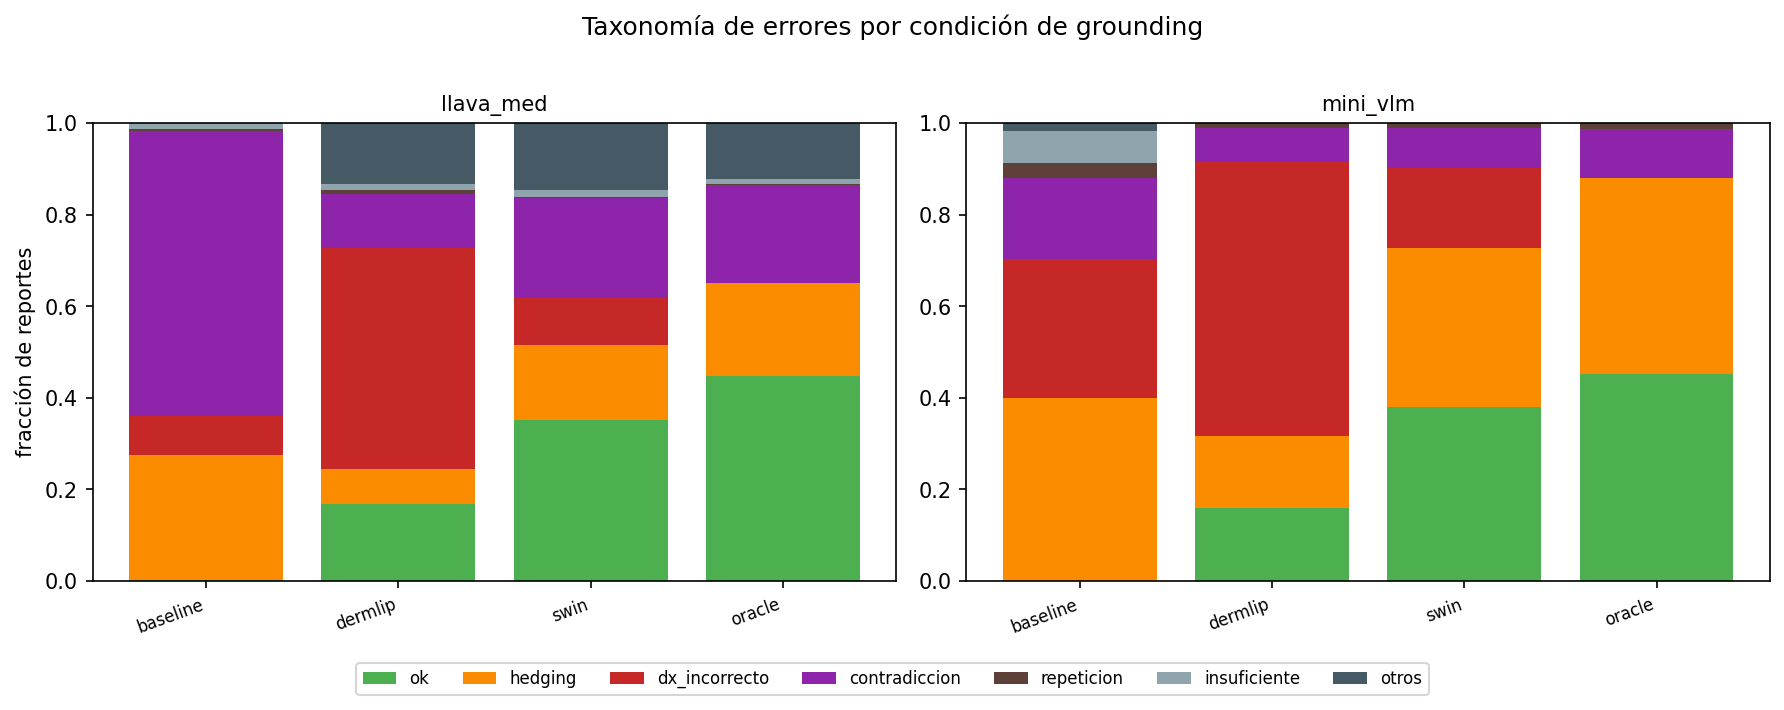
\includegraphics[width=\textwidth]{P05_errors.png}
  \caption{Distribución del tipo de error principal por condición de \emph{grounding}. El \emph{grounding}
  bueno reduce \emph{dx incorrecto} y \emph{contradicción} y aumenta los reportes \emph{ok}; uno malo
  (DermLIP) dispara \emph{dx incorrecto}; el \emph{hedging} persiste aun con el oracle.}
  \label{fig:taxonomia}
\end{figure}

\subsection{Un generador derm-especializado: SkinVL}
\label{sec:skinvl}
¿La especialización que rescató la \emph{clasificación} (DermLIP) ayuda también en la \emph{generación}?
Se integró \textbf{SkinVL-MM} —un VLM derm-especializado (LLaVA-Med v1.5 ajustado sobre MM-Skin), de la
misma familia de modelos que aparece como SOTA de clasificación en el Cuadro~\ref{tab:sota_clasif}
(SkinVL-Pub/SkinVL-PubMM, otros \emph{checkpoints} de~\cite{zeng2025mmskin})— al mismo
ensamble (Cuadro~\ref{tab:skinvl}). Tres observaciones:
\begin{itemize}[leftmargin=1.6em]
  \item \textbf{Sin grounding sufre un \emph{colapso de modo}:} el $72\%$ de sus reportes son
  \emph{idénticos} (solo $72$ respuestas únicas entre las $1503$ imágenes) —una respuesta memorizada de
  su entrenamiento clínico en MM-Skin, p.ej.\ ``tinea corporis''—, por lo que casi nunca menciona la
  clase correcta (consistencia $0.00$). No es que ``genere peor'' que los VLMs generales —que producen
  texto \emph{variado} ($400/400$ reportes únicos)—: es que, aplicado \emph{fuera de su distribución de
  entrenamiento} (MM-Skin clínico $\to$ HAM dermatoscópico) y sin un diagnóstico que lo ancle, se refugia
  en una respuesta constante. La especialización sobre otra distribución de imágenes no transfiere por sí
  sola. \emph{El colapso no es un artefacto del prompt}: al reformular la instrucción (pidiendo
  explícitamente un diagnóstico, o dándole un rol clínico) el modelo sigue colapsando, solo que a un
  diagnóstico distinto —``lichen planus pigmentosus'' en el $33$--$56\%$ de los casos—. Tanto ``tinea
  corporis'' como ``lichen planus pigmentosus'' \emph{no pertenecen a las 7 clases de HAM}: SkinVL emite
  diagnósticos de la distribución de MM-Skin casi sin mirar la imagen, lo que confirma el \emph{mismatch de
  distribución} como causa del colapso.
  \item \textbf{Con grounding alcanza el nivel de Mini-VLM} (Swin $0.80$, oracle $1.00$) y supera a
  LLaVA-Med; la propagación de la calidad del clasificador es monótona.
  \item \textbf{No hace \emph{hedging}} —a diferencia de LLaVA-Med y Mini-VLM, que \emph{hedean} entre el $20$ y
  el $43\%$ de las veces—. Es tentador atribuirlo a que la especialización lo vuelve \emph{decisivo}, pero
  hay una explicación alternativa igual de consistente con la evidencia: el mismo \emph{colapso de modo}
  documentado más arriba (reportes cortos y repetitivos, ajenos a la variedad clínica real) produce, como
  efecto colateral, la ausencia de hedging —un modelo que emite una respuesta fija y escueta no tiene
  margen textual para dudar—. El precio, en cualquiera de las dos lecturas, es que sus reportes son
  \emph{escuetos} (\emph{entity recall} $0.33$–$0.50$ vs $\sim0.77$): esencialmente enuncia el diagnóstico
  sin elaborarlo.
\end{itemize}

\begin{table}[H]
  \centering
  \caption{Diagnostic consistency (report-only) por condición de grounding: SkinVL vs los VLMs generales,
  sobre el \textbf{test completo ($n=1503$)} para los tres. El $\approx$0.00
  del baseline de SkinVL no es un error: es el colapso de modo —solo $3$ de las $1503$ imágenes reciben un
  reporte que menciona la clase correcta (consistency $0.002$)—, porque el modelo repite un diagnóstico
  fijo fuera de las clases de HAM (ver texto). Las exactitudes de clasificación entre paréntesis
  ($0.80$/$0.38$) son las del checkpoint usado como ancla (single-view), como en el Cuadro~\ref{tab:ensamble}.}
  \label{tab:skinvl}
  \begin{tabular}{lccc}
    \toprule
    \textbf{Condición} & \textbf{SkinVL} & \textbf{LLaVA-Med} & \textbf{Mini-VLM} \\
    \midrule
    baseline (sin grounding) & $\approx$0.00 & 0.65 & 0.25 \\
    DermLIP (clasif.\ 0.38)  & 0.43 & 0.45 & 0.50 \\
    Swin (clasif.\ 0.80)     & \textbf{0.80} & \textbf{0.70} & \textbf{0.81} \\
    \midrule
    \textit{oracle (gt) --- cota superior} & \textit{1.00} & \textit{0.85} & \textit{1.00} \\
    \bottomrule
  \end{tabular}
\end{table}

\subsection{¿Cuánto aporta la imagen? Ablaciones del ensamble}
\label{sec:ablaciones}
Dos ablaciones aíslan el rol de cada componente del pipeline. Se aplican a los \textbf{tres generadores}
(SkinVL, LLaVA-Med, Mini-VLM), midiendo en cada caso la \emph{diagnostic consistency}
(Cuadro~\ref{tab:ablaciones}).

\begin{table}[H]
  \centering
  \caption{Ablaciones del ensamble sobre los tres generadores (\emph{diagnostic consistency}). P1.2:
  con grounding \emph{oracle} (dx correcto), con imagen vs.\ con imagen neutra. P1.3: con un dx
  \emph{incorrecto} inyectado, consistencia respecto del GT. SkinVL sobre el test completo ($n{=}1503$);
  LLaVA-Med y Mini-VLM sobre $n{=}400$.}
  \label{tab:ablaciones}
  \begin{tabular}{lccc}
    \toprule
    & \textbf{SkinVL} & \textbf{LLaVA-Med} & \textbf{Mini-VLM} \\
    \midrule
    Oracle, con imagen        & \textbf{1.00} & 0.85 & \textbf{1.00} \\
    Oracle, \emph{sin} imagen & 0.97 & \textbf{1.00} & \textbf{1.00} \\
    \quad$\Delta$ (P1.2 imagen-vs-dx) & $+0.03$ & $-0.15$ & $0.00$ \\
    \addlinespace
    dx-erróneo (P1.3)         & 0.11 & 0.07 & 0.07 \\
    \bottomrule
  \end{tabular}
\end{table}

\paragraph{¿Aporta la imagen una vez conocido el diagnóstico?} Se generó el reporte con \emph{grounding} oracle
pero \emph{reemplazando la imagen por una imagen neutra}. Quitar la imagen \textbf{no mejora la
fidelidad en ninguno} de los tres: SkinVL apenas cae ($\Delta=0.03$), Mini-VLM queda \emph{idéntico}
($\Delta=0.00$) y, de forma reveladora, LLaVA-Med \emph{sube} de $0.85$ a $1.00$ ($\Delta=-0.15$) —dado el
texto del diagnóstico, lo nombra siempre; cuando además \emph{ve} la imagen, la evidencia visual a veces
lo hace dudar y desviarse—. Bajo este protocolo, entonces, la contribución de la señal visual a la
\emph{fidelidad diagnóstica} del reporte es mínima: dado el diagnóstico, la imagen no ayuda a nombrarlo y
en el mejor caso es neutra.

Esto \textbf{no equivale a afirmar que el generador ignore la imagen}, y los mismos reportes permiten
precisar qué sí hace con ella. Sin imagen, todos los reportes de una misma clase son \emph{idénticos}
(similitud de Jaccard intra-clase $1.00$ en ambos modelos: un único texto por diagnóstico); con imagen,
el $99\%$ de los reportes es distinto y la similitud intra-clase cae a $0.36$ (Mini-VLM) y $0.28$
(LLaVA-Med). En Mini-VLM la imagen además sostiene la riqueza del reporte: el \emph{clinical entity
recall} baja de $0.79$ a $0.38$ al quitarla. Es decir, la imagen \textbf{no cambia qué diagnóstico se
redacta, pero sí qué se describe} de cada lesión. Lo que las ablaciones permiten afirmar es acotado: la
señal visual aporta poco a la fidelidad diagnóstica en estas condiciones, no que el modelo carezca de todo
uso de información visual.

\paragraph{¿Qué hace con un diagnóstico erróneo?} Al inyectar un diagnóstico \emph{incorrecto} (una clase
confundible), la consistencia respecto del \emph{gt} se derrumba a $0.07$--$0.11$ en los tres modelos: el
generador \textbf{se compromete con el diagnóstico equivocado} y no lo corrige mirando la imagen
(propagación de error total, universal a los tres generadores).

\paragraph{Una simetría con el diagnóstico del colapso.} Vale conectar este resultado con el de la
Sección~\ref{sec:rediag}, porque ambos usan \emph{el mismo recurso experimental} —sustituir la imagen por
una neutra— y revelan la misma propiedad de fondo, aunque con signos opuestos. En \textbf{clasificación},
quitar la imagen no impidió que el VLM siguiera prediciendo: colapsó al $100\%$ en una clase fija, señal de
que su decisión está dominada por el prior del lenguaje más que por la evidencia visual. En
\textbf{generación}, quitar la imagen tampoco degrada la fidelidad: el modelo nombra igual el diagnóstico
que recibe en el texto. Es, en los dos casos, el mismo hecho: \textbf{en lo que respecta al diagnóstico,
el texto pesa más que la señal visual} en estos VLMs —aunque, como se vio, la imagen sí modula la
descripción—. Lo interesante es que esa única propiedad explica a la vez el fracaso y el éxito del sistema.
Como \emph{clasificadores} los inhabilita —sin discriminación visual suficiente no hay diagnóstico posible—;
como \emph{redactores dentro de la cascada} es precisamente lo que los vuelve confiables, porque garantiza
que transcriban con fidelidad el diagnóstico que se les inyecta en lugar de contradecirlo con una lectura
visual propia y poco fiable. La contracara es la propagación de error de la ablación anterior: esa misma
docilidad textual hace que adopten sin resistencia un diagnóstico equivocado.

\paragraph{Consecuencia.} Ambas ablaciones apuntan a lo mismo: \emph{la fidelidad diagnóstica del
ensamble proviene del clasificador, no de la visión del generador}. El VLM generativo actúa como un
\emph{transcriptor} del diagnóstico a prosa clínica. Un experimento adicional lo confirma directamente: el
Cuadro~\ref{tab:plantilla} compara los VLM con una \textbf{plantilla trivial} (clasificador
$\rightarrow$ dx $\rightarrow$ texto fijo con morfología típica de la clase, sin VLM ni costo de
generación). En consistencia diagnóstica, la plantilla \textbf{iguala o supera} a ambos generadores —con
\emph{grounding} Swin empata a Mini-VLM ($0.828$ vs $0.830$) y supera a LLaVA-Med ($0.703$); con oracle
llega a $1.000$—, aunque pierde en riqueza (\emph{entity recall} $\approx 0.42$ vs $0.75$--$0.79$).

\paragraph{¿Qué aporta entonces el VLM?} Si una plantilla alcanza la misma fidelidad diagnóstica, el aporte
del componente generativo \textbf{no es diagnóstico}, y conviene delimitarlo con precisión porque define qué
agrega realmente cada pieza del sistema. El diagnóstico lo produce el clasificador; el VLM aporta tres cosas
que la plantilla no tiene: (i) \textbf{riqueza clínica} —casi duplica la cobertura de entidades
dermatológicas (\emph{entity recall} $0.75$--$0.79$ frente a $0.41$--$0.44$), es decir, además de nombrar la
clase habla de morfología, color, bordes y hallazgos dermatoscópicos—; (ii) \textbf{especificidad por
caso} —la plantilla emite el mismo texto para todas las lesiones de una clase, mientras que el VLM describe
cada imagen: el $99\%$ de sus reportes son distintos, y es precisamente la imagen la que introduce esa
variación, como mostró la ablación anterior—; y (iii) \textbf{lenguaje y estructura de reporte clínico}.
Ninguno de los tres aportes está validado clínicamente en este trabajo: el \emph{entity recall} mide la
presencia de términos, no que la descripción sea correcta para esa lesión en particular, y verificarlo
requiere un especialista. La lectura precisa es, entonces, que \textbf{el clasificador aporta el
diagnóstico y el VLM aporta la descripción}; la \textbf{contribución metodológica es el pipeline en cascada}
que los combina.

\begin{table}[H]
  \centering
  \caption{Plantilla trivial (clasificador $\to$ texto fijo, costo de generación nulo) vs.\ generadores VLM,
  misma métrica y mismas imágenes ($n=400$).}
  \label{tab:plantilla}
  \small
  \begin{tabular}{llcc}
    \toprule
    \textbf{Grounding} & \textbf{Sistema} & \textbf{Diagnostic consistency} & \textbf{Clinical entity recall} \\
    \midrule
    Swin        & Plantilla   & 0.828 & 0.435 \\
                & LLaVA-Med   & 0.703 & 0.754 \\
                & Mini-VLM    & \textbf{0.830} & \textbf{0.766} \\
    \midrule
    Oracle (gt) & Plantilla   & \textbf{1.000} & 0.412 \\
                & LLaVA-Med   & 0.845 & 0.762 \\
                & Mini-VLM    & \textbf{1.000} & \textbf{0.787} \\
    \bottomrule
  \end{tabular}
\end{table}

\subsection{Grounding por recuperación (RAG)}
\label{sec:rag}
Si la fidelidad la aporta el \emph{diagnóstico} y no la visión del generador, surge una pregunta natural:
¿hace falta un clasificador \emph{entrenado} para producir ese diagnóstico, o alcanza con
\emph{recuperar} casos parecidos? Se probó un \emph{grounding no paramétrico} por recuperación
(\emph{retrieval-augmented generation}, RAG): para cada imagen de test se buscan los $k=3$ casos de
entrenamiento visualmente más cercanos en el espacio de embeddings de DermLIP y se inyecta su diagnóstico
como contexto (``casos similares fueron diagnosticados como\dots''), sin intervención de un clasificador.
El índice contiene solo imágenes de entrenamiento de la partición por lesión; el voto de los tres
vecinos (un \emph{kNN} sobre embeddings DermLIP) acierta el $78\%$ del test.

\emph{Actualización (11/10/2026).} La versión anterior de esta sección usaba un índice construido sobre la
partición por imagen (con fuga: el voto kNN acertaba el $83\%$), el ancla Swin anterior y $n=400$. Se
regeneró (job 1179315, \texttt{rag\_les\_resul\_20261011.md}) con el índice por lesión, el ancla nueva, el
test completo y la métrica oficial (solo reporte, \emph{matcher} estricto).

El Cuadro~\ref{tab:rag} compara, sobre Mini-VLM, el RAG-only y el \emph{grounding} clásico. Tres hallazgos:
(i) el \textbf{RAG-only rescata frente a no anclar pero no reemplaza al clasificador}: lleva la consistencia
de $0.163$ a $0.669$ ($+0.506$ [$+0.476$, $+0.534$]) pero queda $-0.180$ [$-0.206$, $-0.155$] por debajo del
\emph{grounding} con Swin; (ii) \textbf{el generador pierde información de los vecinos}: imprimir el voto kNN
sin generador da $0.781$, y el generador que recibe ese contexto queda $-0.112$ por debajo, porque cuando los
vecinos no coinciden nombra varias clases o una distinta; (iii) \textbf{sumar RAG sobre el clasificador
aporta poco}: $+0.013$ [$+0.007$, $+0.019$], y esa ganancia viene de nombrar la clase de los vecinos además
de la del ancla (la consistencia exclusiva, que exige nombrar solo la clase verdadera, queda $-0.055$ por
debajo de imprimir el diagnóstico de Swin). La versión anterior leía el RAG-only como ``casi igual al
clasificador''; con el índice sin fuga esa lectura no se sostiene.

\begin{table}[H]
  \centering
  \caption{Grounding por recuperación (RAG) vs.\ grounding por clasificador, sobre Mini-VLM ($n=1503$,
  índice y ancla de la partición por lesión; consistencia diagnóstica oficial: solo reporte, \emph{matcher}
  estricto). ``Exclusiva'' exige nombrar la clase verdadera y ninguna otra. Las filas ``impreso'' no usan
  generador: el reporte es solo el diagnóstico.}
  \label{tab:rag}
  \begin{tabular}{lcc}
    \toprule
    \textbf{Condición} & \textbf{Consistencia} & \textbf{Exclusiva} \\
    \midrule
    Baseline (sin contexto)        & 0.163 & 0.045 \\
    RAG-only (recuperación)        & 0.669 & 0.500 \\
    Voto kNN impreso               & 0.781 & 0.781 \\
    Grounding Swin                 & 0.849 & 0.757 \\
    Swin impreso                   & 0.847 & \textbf{0.847} \\
    Grounding Swin + RAG           & \textbf{0.862} & 0.792 \\
    \bottomrule
  \end{tabular}
  \\[2pt]
  {\footnotesize El oracle (recibe el dx verdadero, no es un sistema usable) es la cota superior del
  \emph{grounding} y se excluye de la comparación entre condiciones candidatas.}
\end{table}

\subsection{Ensamble consciente de la incertidumbre}
\label{sec:incertidumbre}
El ensamble en cascada tiene un riesgo estructural: transmite al generador una etiqueta diagnóstica
\emph{dura}, de modo que un error del clasificador se propaga al reporte con falso aplomo
(Sección~\ref{sec:ablaciones}). La calibración (Sección~\ref{sec:calib}) mostró además que la probabilidad
cruda del clasificador no es un estimador de certeza confiable. La respuesta es un ensamble
\textbf{consciente de la incertidumbre} que, en vez de comprometerse siempre con un único diagnóstico,
\emph{modula su salida según cuán seguro está}: afirma cuando hay confianza, ofrece un \textbf{diferencial}
cuando duda, y se \textbf{abstiene (deriva a un especialista)} cuando la ambigüedad es máxima.

\paragraph{Cómo decide, y por qué no con la softmax.} La señal natural para medir confianza sería la
probabilidad del clasificador, pero la Sección~\ref{sec:calib} mostró que \emph{no sirve} como estimador de
certeza: los modelos están mal calibrados (ECE $0.19$--$0.39$) y de forma sistemáticamente sub-confiada, de
modo que el valor absoluto de la softmax no es interpretable como probabilidad de acierto; al usarla para
rutear, la relación entre confianza y exactitud no resulta monótona y el umbral no separa bien los casos
fáciles de los ambiguos. El ruteo usa por eso una señal distinta: el \textbf{acuerdo entre dos
clasificadores especializados baratos}, el supervisado (Swin) y un \emph{kNN} sobre los embeddings de
DermLIP (la recuperación de la Sección~\ref{sec:rag}). Funciona por dos razones. Primero, porque los dos
sistemas tienen \emph{sesgos inductivos y datos de entrenamiento distintos} —Swin ajusta fronteras de
decisión de extremo a extremo sobre HAM10000, mientras que el \emph{kNN} es no paramétrico y opera sobre
una representación contrastiva preentrenada en Derm1M—, de manera que sus errores son en buena medida
independientes: que coincidan es evidencia de que el caso es inequívoco, y que discrepen señala ambigüedad
genuina en vez de ruido de un único modelo. Segundo, y decisivo aquí, porque la señal usa solo las
\emph{decisiones} de ambos y no sus probabilidades, por lo que es \textbf{inmune a la mala calibración}
que invalida a la softmax. Las reglas
(sobre las 1503 imágenes de test, Cuadro~\ref{tab:incertidumbre}; esquema en la
Figura~\ref{fig:incertidumbre}) son: (i)~\textbf{afirmativo} si los dos
coinciden; (ii)~\textbf{abstención} si difieren \emph{y} los tres vecinos recuperados son de clases todas
distintas (sin consenso); (iii)~\textbf{diferencial} en el resto (difieren pero hay consenso parcial),
presentando ambos candidatos. Para cada nivel se reporta la \textbf{cobertura del gt}: la fracción de
casos en los que el diagnóstico verdadero queda cubierto por la salida del nivel —exactitud en el nivel
afirmativo (gt$=$dx) y presencia del gt entre los candidatos en el diferencial.

\begin{table}[H]
  \centering
  \caption{Ensamble consciente de la incertidumbre (3 niveles) sobre HAM10000 test ($n=1503$). ``Cobertura''
  $=$ exactitud (nivel afirmativo, gt$=$dx) o fracción con gt entre los candidatos (diferencial/abstención).}
  \label{tab:incertidumbre}
  \begin{tabular}{lccl}
    \toprule
    \textbf{Nivel} & \textbf{Imágenes} & \textbf{Cobertura del gt} & \textbf{Acción} \\
    \midrule
    Afirmativo (acuerdo)        & 1111 (74\%) & \textbf{0.944} & reporte definitivo \\
    Diferencial (consenso parc.) & 334 (22\%)  & 0.898 & diferencial \{Swin, kNN\} \\
    Abstención (sin consenso)   & 58 (4\%)    & 0.793 & \emph{derivar a especialista} \\
    \midrule
    \textit{Total no derivado}  & \textit{1445 (96\%)} & \textbf{0.934} & (afirmativo $+$ diferencial) \\
    \bottomrule
  \end{tabular}
\end{table}

\begin{figure}[htbp]
\centering
\begin{tikzpicture}[
  box/.style={rectangle, rounded corners, draw, thick, align=center, minimum height=1.4cm,
              font=\small, text width=3.4cm},
  >=Stealth]
  \node[box, fill=gray!8, text width=3.0cm] (sig) {Señal de acuerdo\\ Swin \emph{vs} kNN-DermLIP};
  \node[box, draw=orange!85!black, right=4.6cm of sig] (dif)
       {\textbf{Diferencial} — 22\,\%\\ cobertura $0.898$\\ enuncia \{Swin, kNN\}};
  \node[box, draw=green!45!black, above=0.9cm of dif] (aff)
       {\textbf{Afirmativo} — 74\,\%\\ cobertura $0.944$\\ \emph{reporte definitivo}};
  \node[box, draw=red!70!black, below=0.9cm of dif] (abs)
       {\textbf{Abstención} — 4\,\%\\ cobertura $0.793$\\ \emph{deriva a especialista}};
  \draw[->] (sig.east) to[bend left=18]  node[pos=0.6,above,font=\scriptsize,sloped]{coinciden} (aff.west);
  \draw[->] (sig.east) -- node[midway,above,font=\scriptsize]{consenso parcial} (dif.west);
  \draw[->] (sig.east) to[bend right=18] node[pos=0.6,below,font=\scriptsize,sloped]{sin consenso} (abs.west);
\end{tikzpicture}
\caption{Ensamble consciente de la incertidumbre. El acuerdo entre dos clasificadores especializados
baratos (Swin supervisado y un \emph{kNN} sobre embeddings de DermLIP) rutea cada caso a uno de tres
niveles: afirmar, dar un diferencial o derivar. Porcentajes y cobertura del gt sobre HAM10000 test
($n=1503$, Cuadro~\ref{tab:incertidumbre}). En conjunto, el sistema deja el diagnóstico correcto entre
sus salidas en el $93.4\%$ de los casos no derivados.}
\label{fig:incertidumbre}
\end{figure}

El resultado es que el sistema \textbf{pone el diagnóstico correcto ``sobre la mesa'' en el $93.4\%$ de los
casos no derivados} (afirma bien, o incluye el gt entre dos candidatos cuando duda), frente a un
\emph{grounding} forzado que emite un único diagnóstico y acierta $\approx$80\%. La \textbf{abstención}
aísla el $4\%$ de máxima ambigüedad —donde incluso el par de candidatos contiene el gt solo el $79\%$— y lo
deriva, evitando el reporte confiadamente incorrecto.

\paragraph{Validación end-to-end (sobre los reportes generados).} La cobertura anterior es del
\emph{componente de decisión}; para verificar que el \emph{texto} la realiza, se generaron los reportes de
cada nivel (afirmativo $=$ grounding; diferencial $=$ se enuncian ambos candidatos; abstención $=$ sin
reporte). En el subconjunto diferencial, el reporte diferencial \textbf{menciona el diagnóstico correcto el
$90\%$ de las veces, frente al $39\%$ del grounding forzado} sobre esas mismas imágenes —donde el
clasificador se equivoca—. Agregando los tres niveles, la \emph{diagnostic consistency} del \textbf{sistema
completo} sobre los casos no derivados sube de $\mathbf{0.82}$ (grounding simple) a $\mathbf{0.94}$
(Cuadro~\ref{tab:incertidumbre_e2e}). La mejora es \textbf{significativa} (\emph{bootstrap} pareado,
$2000$ remuestreos): $\Delta=+0.118$ $[0.101,\,0.134]$ sobre los $1445$ casos no derivados, y
$\Delta=+0.509$ $[0.452,\,0.566]$ del reporte diferencial sobre el forzado en el subconjunto diferencial
($n=334$); ambos intervalos del $95\%$ excluyen el cero. Así, la calibración deja de ser un análisis aparte y se
\emph{integra al sistema}: es la lógica que decide cuándo comprometerse, cuándo dar un diferencial y cuándo
callar y derivar.

\paragraph{Réplica con el segundo generador.} Para descartar que la mejora sea una particularidad de
Mini-VLM se repitió la validación con \textbf{LLaVA-Med}, con el mismo ruteo, las mismas imágenes y los
mismos hiperparámetros de generación. Como el componente de decisión es independiente del generador, solo
hizo falta generar los $334$ reportes del nivel diferencial: el nivel afirmativo reutiliza los reportes de
\emph{grounding}-Swin ya existentes y el de abstención no produce texto. El resultado se replica con una
magnitud casi idéntica (Cuadro~\ref{tab:incertidumbre_e2e}): la consistencia sobre los casos no derivados
sube de $0.706$ a $0.831$ ($\Delta=+0.125$ $[0.109,\,0.143]$), y en el subconjunto diferencial el reporte
diferencial nombra el diagnóstico correcto el $89.5\%$ de las veces frente al $35.3\%$ del forzado. Que el
salto absoluto sea prácticamente el mismo en ambos modelos ($+0.118$ y $+0.125$) pese a que parten de niveles
muy distintos es coherente con dónde se origina la mejora: en la \emph{decisión} de rutear, que es común a
los dos, y no en la capacidad de redacción de cada generador. El nivel de partida más bajo de LLaVA-Med
refleja lo ya visto en el Cuadro~\ref{tab:ensamble}: aun con el diagnóstico en el \emph{prompt}, lo nombra
con menos regularidad que Mini-VLM.

\paragraph{Cómo leer el $0.94$.} Es tentador comparar ese valor con una exactitud, pero \textbf{no es una
exactitud multiclase} y su definición tiene tres particularidades que conviene explicitar. Primero, es una
\emph{diagnostic consistency}: la proporción de reportes que mencionan el diagnóstico verdadero, no la
proporción de casos en que el sistema emite un único diagnóstico correcto. Segundo, mezcla dos tipos de
salida: en el nivel afirmativo ($77\%$ de los no derivados) el reporte nombra un solo diagnóstico y la
consistencia es $0.951$ —prácticamente la exactitud del clasificador en ese subconjunto, $0.944$—, pero en
el nivel diferencial ($23\%$) nombra \emph{dos} candidatos y cuenta como consistente si el verdadero es uno
de ellos ($0.901$), un criterio análogo a una exactitud \emph{top-2}. Tercero, se calcula \emph{excluyendo}
el $4\%$ de casos derivados, que son justamente los más difíciles. Por eso la comparación honesta no es
$0.94$ contra la exactitud del ancla ($0.795$), sino contra el \emph{grounding} simple \emph{sobre las mismas
imágenes} ($0.82$), y conviene acompañarla del valor sobre la cohorte completa, contando cada derivación
como un reporte sin diagnóstico: $\mathbf{0.904}$ frente a $0.812$ (Mini-VLM) y $0.799$ frente a $0.696$
(LLaVA-Med). Lo que el $0.94$ afirma, entonces, es que \emph{cuando el sistema entrega un reporte}, este
contiene el diagnóstico correcto —solo o junto a un segundo candidato— en el $94\%$ de los casos; no que
el sistema diagnostique correctamente al $94\%$ de los pacientes.

\paragraph{¿Reduce los errores peligrosos?} La consistencia agregada no distingue \emph{qué tipo} de error
se comete, y clínicamente no todos pesan igual (Sección~\ref{sec:taxonomia}). Se aplicó por eso la taxonomía
de errores a ambos sistemas sobre las mismas imágenes (Cuadro~\ref{tab:taxonomia_incert}), con un ajuste
necesario: la regla que marca \emph{contradicción} cuando el texto menciona dos clases no puede aplicarse al
reporte diferencial, que enuncia dos candidatos \emph{por diseño}; para ese nivel se cuenta como correcto
(\emph{ok diferencial}) si el diagnóstico verdadero está entre los candidatos, y como \emph{dx incorrecto}
si no lo está. Con Mini-VLM el resultado es contundente: el \textbf{diagnóstico incorrecto —el error clínicamente grave—
cae del $19.0\%$ al $6.6\%$} sobre las no derivadas. Y las $58$ imágenes derivadas habrían producido
$26$ reportes con diagnóstico equivocado bajo \emph{grounding} forzado: al abstenerse, el sistema los evita
por completo. Sobre la cohorte completa de $1503$ pacientes la tasa de diagnóstico incorrecto pasa de
$\mathbf{20.0\%}$ ($301/1503$) a $\mathbf{6.3\%}$ ($95/1503$), una \textbf{reducción del $68\%$}.
La mejora no es solo un traslado de errores a categorías más benignas: la fracción de reportes
\emph{diagnósticamente correctos} —contando el diferencial como acierto cuando el gt figura entre los
candidatos— sube de $38.4\%$ a $\mathbf{51.1\%}$, de modo que el sistema no se limita a evitar
afirmaciones falsas sino que además acierta más seguido.

Con \textbf{LLaVA-Med} el patrón se repite: el diagnóstico incorrecto \textbf{se reduce a la mitad}
($13.5\% \rightarrow 7.0\%$ sobre las no derivadas; $14.2\% \rightarrow 6.7\%$ sobre la cohorte completa,
contando los $18$ errores que evita la derivación) y los reportes correctos suben de $35.6\%$ a $49.0\%$.
La réplica corrige, además, una lectura previa. Con Mini-VLM la \textbf{repetición empeora}
($0.3\% \rightarrow 4.3\%$) y parecía natural atribuirlo al formato —enumerar dos candidatos favorecería el
bucle de texto—; pero con LLaVA-Med la repetición se mantiene en niveles marginales ($0.1\% \rightarrow
0.3\%$) con el mismo formato diferencial. La amplificación es, por lo tanto, \textbf{propia de Mini-VLM} y
no una consecuencia inevitable del ruteo. LLaVA-Med tiene, en cambio, su propio perfil de error: más
contradicciones y reportes que no nombran ninguna clase (\emph{otros}), en línea con su estilo más verboso.

\begin{table}[H]
  \centering
  \caption{Taxonomía de errores del \emph{grounding} simple forzado (``simple'') vs.\ el ensamble consciente
  de la incertidumbre (``avanzado''), con los dos generadores, sobre las mismas $1445$ imágenes no derivadas.
  En el nivel diferencial, mencionar los dos candidatos es el comportamiento esperado: se contabiliza como
  \emph{ok diferencial} cuando el gt está entre ellos. Las categorías particionan el conjunto (suman $100\%$
  en cada columna); \emph{ok} y \emph{ok diferencial} son componentes de \emph{Correcto (total)}. Las
  flechas indican la dirección deseable ($\uparrow$ más es mejor, $\downarrow$ menos es mejor).}
  \label{tab:taxonomia_incert}
  \small
  \resizebox{\textwidth}{!}{%
  \begin{tabular}{lcccc}
    \toprule
    & \multicolumn{2}{c}{\textbf{Mini-VLM}} & \multicolumn{2}{c}{\textbf{LLaVA-Med}} \\
    \cmidrule(lr){2-3}\cmidrule(lr){4-5}
    \textbf{Categoría} & \textbf{Simple} & \textbf{Avanzado} & \textbf{Simple} & \textbf{Avanzado} \\
    \midrule
    \quad ok                              & 555 (38.4\%) & 498 (34.5\%) & 514 (35.6\%) & 483 (33.4\%) \\
    \quad ok diferencial                  & ---          & 240 (16.6\%) & ---          & 225 (15.6\%) \\
    \textbf{Correcto (total)} $\uparrow$  & 555 (38.4\%) & \textbf{738 (51.1\%)} & 514 (35.6\%) & \textbf{708 (49.0\%)} \\
    \midrule
    hedging $\downarrow$                  & 491 (34.0\%) & \textbf{436 (30.2\%)} & 257 (17.8\%) & \textbf{239 (16.5\%)} \\
    dx incorrecto $\downarrow$            & 275 (19.0\%) & \textbf{95 (6.6\%)}   & 195 (13.5\%) & \textbf{101 (7.0\%)} \\
    contradicción $\downarrow$            & 120 (8.3\%)  & \textbf{114 (7.9\%)}  & 257 (17.8\%) & \textbf{221 (15.3\%)} \\
    repetición $\downarrow$               & \textbf{4 (0.3\%)} & 62 (4.3\%)      & \textbf{2 (0.1\%)} & 5 (0.3\%) \\
    insuficiente $\downarrow$             & 0 (0.0\%)    & 0 (0.0\%)    & 45 (3.1\%)   & \textbf{25 (1.7\%)} \\
    otros (sin clase) $\downarrow$        & 0 (0.0\%)    & 0 (0.0\%)    & 175 (12.1\%) & \textbf{146 (10.1\%)} \\
    \bottomrule
  \end{tabular}%
  }
\end{table}

\paragraph{¿Dónde duda el sistema?} El Cuadro~\ref{tab:ruteo_clase} desagrega el ruteo por clase
diagnóstica y revela un comportamiento \textbf{consciente del riesgo que no fue diseñado explícitamente}:
la señal de acuerdo afirma con confianza donde la tarea es fácil y benigna —nevo $81.3\%$ y lesión vascular
$90.9\%$ de casos afirmativos, ambas de morfología distintiva— y se vuelve \textbf{marcadamente más cauta en
melanoma}, donde solo el $52.7\%$ se afirma: el $40.1\%$ se enuncia como diferencial y un $7.2\%$ se deriva.
Es decir, \textbf{el sistema no afirma melanoma a ciegas}: ante duda pone el melanoma sobre la mesa junto al
otro candidato, o pide criterio humano. El mecanismo detrás de esa cautela se ve al inspeccionar
\emph{con qué} se confunde: de los $67$ melanomas ruteados a diferencial, $32$ ($48\%$) tienen como par de
candidatos \{melanoma, nevo\} y otros $13$ ($19\%$) \{melanoma, queratosis benigna\}; es decir, dos tercios
de las discrepancias reproducen \textbf{los diagnósticos diferenciales clínicos canónicos} del melanoma
—precisamente las lesiones pigmentadas con las que comparte apariencia—. El desacuerdo entre los dos
clasificadores no es entonces ruido: aparece donde las clases genuinamente se solapan en la imagen, que es
la razón por la cual sirve como estimador de ambigüedad. Dermatofibroma, la clase más rara ($n=17$), concentra la mayor tasa
de abstención ($35.3\%$), coherente con su escasez en el entrenamiento. Es el patrón que se buscaría en un
entorno clínico —cautela donde el error es caro, decisión donde el caso es claro—, aunque que efectivamente
resulte útil para un especialista es algo que estas métricas no pueden establecer.

\begin{table}[H]
  \centering
  \caption{Ruteo del ensamble consciente de la incertidumbre por clase diagnóstica (HAM10000 test,
  $n=1503$). Porcentajes por fila. El sistema afirma más en las
  clases fáciles/benignas y deriva o da diferencial con más frecuencia en melanoma y en las clases raras.}
  \label{tab:ruteo_clase}
  \begin{tabular}{lrccc}
    \toprule
    \textbf{Clase} & \textbf{n} & \textbf{Afirmativo} & \textbf{Diferencial} & \textbf{Abstención} \\
    \midrule
    Nevo (NV)                  & 1006 & 81.3\% & 17.4\% & 1.3\% \\
    Melanoma (MEL)             & 167  & 52.7\% & \textbf{40.1\%} & 7.2\% \\
    Queratosis benigna (BKL)   & 165  & 58.2\% & 31.5\% & 10.3\% \\
    Basocarcinoma (BCC)        & 77   & 72.7\% & 22.1\% & 5.2\% \\
    Queratosis actínica (AKIEC)& 49   & 55.1\% & 34.7\% & 10.2\% \\
    Lesión vascular (VASC)     & 22   & \textbf{90.9\%} & 4.5\% & 4.5\% \\
    Dermatofibroma (DF)        & 17   & 35.3\% & 29.4\% & \textbf{35.3\%} \\
    \bottomrule
  \end{tabular}
\end{table}

\begin{table}[H]
  \centering
  \caption{Validación end-to-end del ensamble consciente de la incertidumbre con los dos generadores, sobre
  las mismas imágenes. Todas las filas son \emph{diagnostic consistency}; $\Delta$ con IC del $95\%$
  (\emph{bootstrap} pareado, $2000$ remuestreos). En el nivel diferencial el reporte nombra \emph{dos}
  candidatos, por lo que estos valores no equivalen a una exactitud de diagnóstico único (ver texto).}
  \label{tab:incertidumbre_e2e}
  \small
  \begin{tabular}{lcc}
    \toprule
    \textbf{Sistema} & \textbf{Mini-VLM} & \textbf{LLaVA-Med} \\
    \midrule
    \multicolumn{3}{@{}l}{\itshape Casos no derivados ($n=1445$)} \\
    Grounding simple (forzado)                      & 0.822 & 0.706 \\
    Pipeline avanzado (afirmativo $+$ diferencial)  & \textbf{0.940} & \textbf{0.831} \\
    \quad $\Delta$ [IC 95\%]                        & $+0.118$ [$0.101$, $0.134$] & $+0.125$ [$0.109$, $0.143$] \\
    \midrule
    \multicolumn{3}{@{}l}{\itshape Solo el subconjunto diferencial ($n=334$)} \\
    Grounding forzado (se compromete con Swin)      & 0.392 & 0.353 \\
    Reporte diferencial (\{Swin, kNN\})             & \textbf{0.901} & \textbf{0.895} \\
    \quad $\Delta$ [IC 95\%]                        & $+0.509$ [$0.452$, $0.566$] & $+0.542$ [$0.485$, $0.602$] \\
    \midrule
    \multicolumn{3}{@{}l}{\itshape Cohorte completa ($n=1503$; una derivación cuenta como reporte sin diagnóstico)} \\
    Grounding simple (forzado)                      & 0.812 & 0.696 \\
    Pipeline avanzado                               & \textbf{0.904} & \textbf{0.799} \\
    \bottomrule
  \end{tabular}
\end{table}

\subsection{Nivel 1 sobre SkinCoT: un \emph{trade-off} de estilo}
\label{sec:skincot}
Esta subsección y los ejemplos cualitativos que siguen vuelven a las condiciones \emph{simples}
(\emph{grounding} baseline/oracle) en lugar del ensamble de 3 niveles de la sección anterior: aquí el
objetivo es aislar el efecto léxico y mostrar patrones de reporte, no re-evaluar el sistema completo, que
ya fue validado \emph{end-to-end} en la Sección~\ref{sec:incertidumbre}. Para evaluar la calidad
lingüística con referencia se usó SkinCoT. Se comparan \textbf{baseline} y
\textbf{oracle} (con \emph{noreasoning}). El Cuadro~\ref{tab:ensamble_skincot} y la Figura~\ref{fig:f3}
muestran un \emph{trade-off}: el \emph{grounding} \textbf{sube} la fidelidad (consistency $0.39 \rightarrow 0.57$)
pero \textbf{baja} la similitud léxica (BLEU-4 $0.10 \rightarrow 0.04$). La razón es estilística: las
referencias de SkinCoT son narrativas \emph{verbosas}, y un reporte conciso se parece menos a ellas
aunque sea diagnósticamente más fiel. Este \emph{trade-off} es evidencia adicional de lo discutido junto al
Cuadro~\ref{tab:sota_gen}: las métricas léxicas (BLEU/ROUGE) penalizan el estilo, no la calidad clínica.
El siguiente contraste lo ilustra:

\begin{figure}[H]
\centering
\fbox{\parbox{0.96\textwidth}{\footnotesize
\textbf{Reporte verboso (baseline, alto solapamiento léxico)} \textemdash\ \itshape ``To analyze the
case I will follow a structured approach to arrive at a logical diagnostic conclusion\dots\ The general
disease category may belong to neoplastic, specifically a lesion that could be benign or malignant\dots''
\upshape (largo, parecido al estilo de la referencia, pero sin comprometerse).\\[4pt]
\textbf{Reporte conciso (oracle/noreasoning, menor solapamiento léxico, mayor fidelidad)} \textemdash\
\itshape ``The diagnosis is a nevus. Brownish pigmentation, regular borders, symmetric\dots'' \upshape
(corto y comprometido).
}}
\caption{Verboso vs.\ conciso: el reporte verboso se parece más a la referencia (mayor BLEU) pero no
concluye; el conciso acierta el diagnóstico (mayor consistency).}
\label{fig:verboso}
\end{figure}

\begin{figure}[H]
\centering
\fbox{\parbox{0.96\textwidth}{\footnotesize
\begin{minipage}[c]{0.22\textwidth}
  \centering
  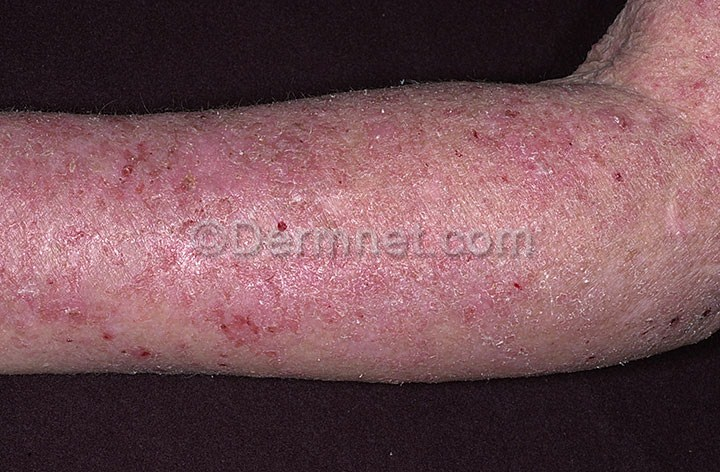
\includegraphics[width=\textwidth]{ej_skincot_human.jpg}\\[2pt]
  {\scriptsize SkinCoT: 03DermatitisArm1\\ \emph{gt}: eczema}
\end{minipage}\hfill
\begin{minipage}[c]{0.73\textwidth}
\textbf{Narrativa de referencia (SkinCoT, certificada por dermatólogos)} \textemdash\ \itshape ``The combination of erythema
$+$ fine scaling $+$ excoriations/crusts $+$ lichenification $+$ intense pruritus is highly characteristic
of chronic eczema, most likely atopic dermatitis\dots\ this presentation is consistent with atopic
dermatitis (eczema). \dots\ I recommend consulting a dermatologist for confirmation and management.''
\upshape\\[4pt]
\textbf{Reporte generado (ensamble, \emph{grounding} oracle)} \textemdash\ \itshape ``The image shows
widespread erythema (redness) with numerous small, raised papules and scattered crusting\dots\ the
surrounding dry, flaky skin indicates chronicity and possible lichenification. The distribution is diffuse,
affecting the entire limb, which is typical for Eczema Photos.''\upshape
\end{minipage}
}}
\caption{Narrativa de referencia de SkinCoT vs.\ reporte generado por el ensamble sobre el
\emph{mismo} caso (Nivel 1). La referencia \textbf{no} es un reporte redactado por un dermatólogo: SkinCoT
la produce con un pipeline de modelos de lenguaje —descripción observacional, borrador de razonamiento
generado \emph{conociendo la etiqueta verdadera} y normalización— que luego \textbf{dermatólogos
certifican y filtran} sobre seis criterios de calidad clínica~\cite{shen2025skincare}. Es, por tanto, una
referencia validada por especialistas, no una redactada por ellos. Ambos identifican los rasgos clave —eritema, descamación,
excoriaciones/costras, liquenificación— y concluyen eczema: la referencia razona el diferencial de forma
narrativa y el generado describe la morfología de manera más directa. ``Eczema Photos'' es el nombre crudo
de la categoría en la taxonomía de SkinCoT, empleada como etiqueta de \emph{grounding}.}
\label{fig:human_vs_gen}
\end{figure}

\begin{table}[H]
  \centering
  \caption{Ensamble sobre SkinCoT (con referencias). El \emph{grounding}+\emph{noreasoning} sube la
  consistencia y baja la similitud léxica.}
  \label{tab:ensamble_skincot}
  \begin{tabular}{lcccc}
    \toprule
    \textbf{Condición} & \textbf{BLEU-4} & \textbf{METEOR} & \textbf{CIDEr} & \textbf{Consistency} \\
    \midrule
    Baseline             & \textbf{0.102} & \textbf{0.330} & \textbf{0.054} & 0.392 \\
    Oracle (noreasoning) & 0.040 & 0.209 & 0.038 & \textbf{0.567} \\
    \bottomrule
  \end{tabular}
\end{table}

Como SkinCoT es el único de los conjuntos usados que trae narrativas de referencia validadas por
dermatólogos, permite además el único contraste \emph{directo} entre reporte de referencia y reporte
generado sobre el mismo caso (Figura~\ref{fig:human_vs_gen}): ambos capturan los mismos hallazgos
morfológicos y concluyen el mismo diagnóstico, con la referencia razonando el diferencial de forma más
narrativa. Cabe precisar el estatus de esa referencia: SkinCoT no contiene reportes \emph{redactados} por
un dermatólogo, sino narrativas producidas por modelos de lenguaje —el borrador de razonamiento se genera
\emph{con la etiqueta verdadera a la vista}— y luego certificadas y filtradas por dermatólogos según seis
criterios de calidad~\cite{shen2025skincare}. Esto acota lo que la comparación demuestra: es un contraste
contra una referencia \emph{validada clínicamente}, no contra la redacción espontánea de un especialista,
y no reemplaza la evaluación por dermatólogo que se discute en las limitaciones.

\paragraph{Comparación con el estado del arte.} A diferencia de la clasificación —donde una métrica
como la exactitud o la sensibilidad macro refleja de forma bastante fiel la calidad del modelo—, en
generación de reportes las métricas más usadas en la literatura son de \emph{similitud léxica} (BLEU,
ROUGE, METEOR), que comparan el texto generado con un reporte de referencia, palabra por palabra. Estas
métricas son \emph{poco representativas} de la calidad clínica de un reporte: por la naturaleza del
lenguaje, un mismo hallazgo puede expresarse de muchas formas igualmente correctas, de modo que un
reporte diagnósticamente acertado pero redactado distinto a la referencia recibe un puntaje bajo (y, a la
inversa, un reporte que copia el estilo pero yerra el diagnóstico puede puntuar alto). Aun así, son el
estándar de comparación del área, por lo que el Cuadro~\ref{tab:sota_gen} las recopila.

Dos cautelas al leer el cuadro: (i) los valores dependen mucho del ajuste al \emph{estilo} del dataset de
referencia —sobre MM-Skin, los VLMs generales obtienen BLEU-4 $\approx 8.9$ y solo el modelo
derm-especializado y ajustado sobre ese corpus (SkinVL-MM) llega a $\approx 22$; sobre datos sintéticos
de texto muy estructurado (DermatoLlama) las cifras se disparan a $\approx 65$—; y (ii) cada fila usa un
dataset, una modalidad y un protocolo distintos (MM-Skin, DERM12345, IU-Xray, corpus privados), por lo
que \textbf{no son comparables entre sí} ni con nuestros números sobre SkinCoT. Por eso este trabajo
prioriza la \emph{fidelidad diagnóstica} (Nivel 2), que mide si el reporte efectivamente acierta el
diagnóstico —dimensión que estas comparativas no capturan.

Nuestros modelos aparecen al pie del Cuadro~\ref{tab:sota_gen}, evaluados sobre MM-Skin (el mismo
\emph{benchmark} que las primeras filas). El contraste es la mejor evidencia del punto anterior: como
fueron entrenados sobre SkinCaRe y se aplican a MM-Skin \emph{sin reajuste}, su BLEU-4 cae a
$\approx 0.1$ —dos órdenes de magnitud por debajo de los modelos ajustados sobre MM-Skin—; sin embargo,
su \emph{BERTScore} ($\approx 67$--$71$), que mide similitud \emph{semántica} y no de palabras exactas,
queda al nivel del SOTA sobre ese mismo \emph{benchmark} ($\approx 67$--$71$). Es decir, el contenido es
comparable pero la redacción difiere: el BLEU castiga la diferencia de estilo, no la de calidad clínica.
Esto confirma por qué la evaluación de Nivel 2 es la métrica decisiva en este trabajo.

\begin{table}[H]
  \centering
  \caption{Estado del arte en generación de reportes dermatológicos según métricas de similitud léxica
  (escala 0--100, salvo donde se indique). Las cifras \textbf{no son directamente comparables entre
  filas}: cada trabajo usa un dataset, una modalidad y un protocolo distintos (incluso métricas
  homónimas difieren, p.\,ej.\ BLEU-4 vs SacreBLEU). Se incluyen como referencia del rango habitual en
  el dominio, no como ranking; el resaltado se limita a cada bloque internamente comparable.
  ``---'' = no reportado.}
  \label{tab:sota_gen}
  \small
  \resizebox{\textwidth}{!}{%
  \begin{tabular}{llcccc}
    \toprule
    \textbf{Fuente} & \textbf{Modelo / dataset} & \textbf{BLEU-4} & \textbf{ROUGE-L} & \textbf{METEOR} & \textbf{BERTScore} \\
    \midrule
    \multicolumn{6}{@{}l}{\itshape Evaluados sobre MM-Skin} \\
    \cite{zeng2025mmskin} & LLaVA-Med-7B (derma.) & 8.88 & 34.83 & 33.74 & 66.60 \\
    \cite{zeng2025mmskin} & SkinVL-MM (derma.) & 21.61 & \textbf{44.70} & \textbf{42.76} & \textbf{71.34} \\
    \cite{zeng2025mmskin} & SkinVL-MM (patología) & \textbf{22.04} & 44.09 & 42.70 & 70.59 \\
    \multicolumn{6}{@{}l}{\itshape Otros datasets (referencia metodológica)} \\
    \cite{AutomatedReport2025} & KD-VLM / dermatosc.\ priv. & 55.59$^{a}$ & 38.28 & --- & 90.25$^{b}$ \\
    \cite{DermatoLlama2025} & DermatoLlama / DERM12345 (sint.) & 65.59 & 93.44$^{c}$ & --- & --- \\
    \cite{PeFoMed2024} & PeFoMed / IU-Xray (radiol.) & --- & 28.60$^{d}$ & 15.70 & --- \\
    \multicolumn{6}{@{}l}{\itshape Este trabajo --- evaluado sobre MM-Skin$^{e}$} \\
    & LLaVA-Med (FT SkinCaRe) & 0.09 & 3.36 & 8.72 & 67.03 \\
    & Mini-VLM (FT SkinCaRe) & \textbf{0.16} & \textbf{5.80} & \textbf{11.21} & \textbf{71.29} \\
    \bottomrule
  \end{tabular}%
  }
  \par\smallskip
  {\footnotesize $^{a}$SacreBLEU (no equivalente a BLEU-4 estándar). $^{b}$BERTScore F1 original $0.9025$
  (escala 0--1). $^{c}$ROUGE inusualmente alto, atribuible a la estructura repetitiva de los datos
  sintéticos. $^{d}$Reportes radiológicos (IU-Xray), no dermatológicos; incluido como referencia de la
  arquitectura VLM$+$LoRA. $^{e}$Nuestros modelos se entrenaron sobre SkinCaRe y se evalúan aquí sobre
  MM-Skin \emph{sin ajuste a ese corpus} (transferencia entre datasets), de ahí los puntajes léxicos muy
  bajos pese a su fidelidad diagnóstica en Nivel 2. Recalculado el 12/10/2026 sin las imágenes sin descripción
  (antes entraban con la referencia ``nan'') y sin los bloques \texttt{<think>}: $n = 6\,590$ (Mini-VLM) y
  $2\,426$ (LLaVA-Med), sobre el archivo completo cortado por tiempo y no sobre la partición de prueba (en
  regeneración, jobs 1179990 y 1179991).\par}
\end{table}

\begin{figure}[H]
  \centering
  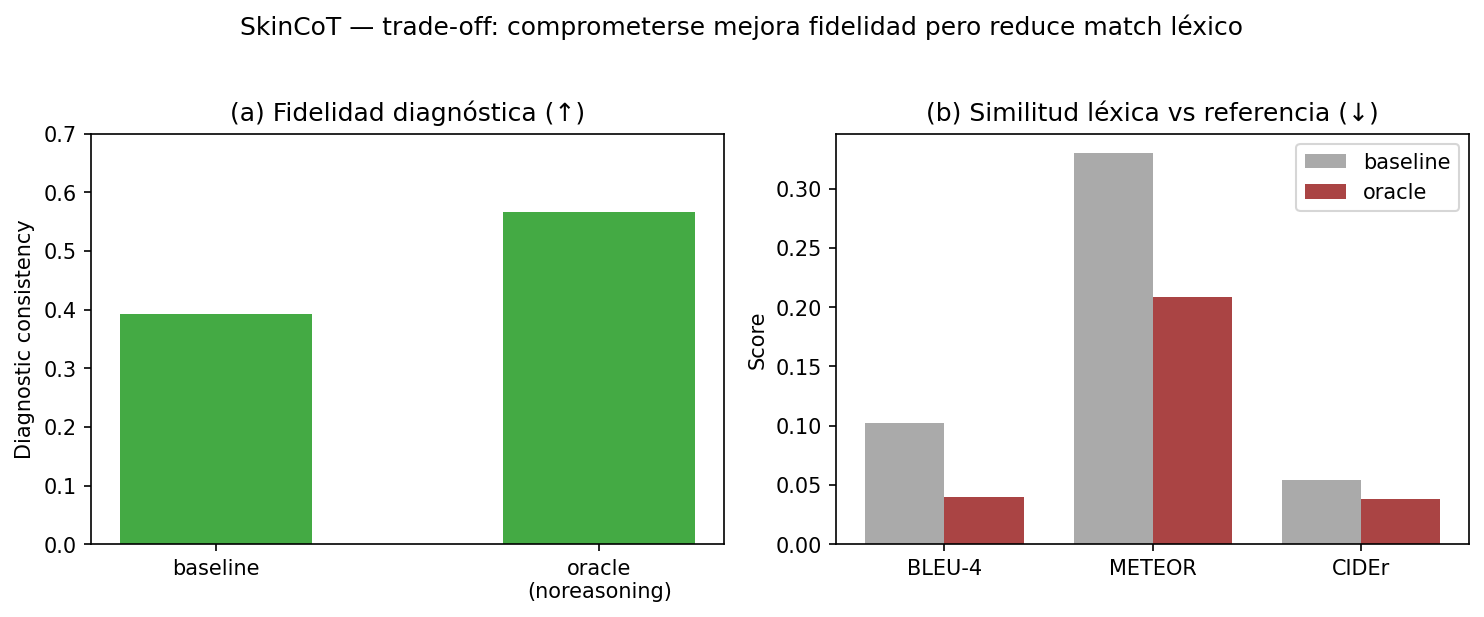
\includegraphics[width=\textwidth]{F3_skincot_tradeoff.png}
  \caption{SkinCoT: (a) la fidelidad diagnóstica sube con el \emph{grounding}; (b) las métricas léxicas
  bajan porque el reporte comprometido es más conciso que la referencia verbosa.}
  \label{fig:f3}
\end{figure}

\subsection{Ejemplos cualitativos: qué distingue un buen reporte}
\label{sec:cualitativo}
Más allá de las métricas, conviene mostrar qué separa un buen reporte de uno malo. Un \textbf{buen
reporte} (i) afirma un diagnóstico, (ii) lo sustenta con rasgos morfológicos coherentes, y (iii) es
conciso y sin contradicciones. Un \textbf{mal reporte} (i) \emph{hedea}, (ii) se compromete con un diagnóstico
\emph{incorrecto}, o (iii) degenera (p.\,ej.\ repite frases). Los Ejemplos de las
Figuras~\ref{fig:ej_grounding} y~\ref{fig:verboso} ya ilustraron (i); las Figuras~\ref{fig:ej_error}
y~\ref{fig:ej_rep} muestran, respectivamente, los riesgos (ii) y (iii).

\begin{figure}[H]
\centering
\fbox{\parbox{0.96\textwidth}{\footnotesize
\textbf{Riesgo (ii): propagación de error.}\\[3pt]
\begin{minipage}[c]{0.22\textwidth}
  \centering
  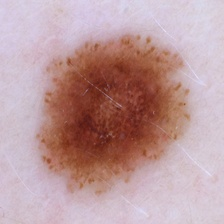
\includegraphics[width=\textwidth]{ej_ISIC_0024317.jpg}\\[2pt]
  {\scriptsize ISIC\_0024317\\ \emph{gt}: nevo\\ DermLIP: melanoma}
\end{minipage}\hfill
\begin{minipage}[c]{0.72\textwidth}
\itshape ``The lesion is a melanoma, characterized by a large, irregularly shaped, dark brown to black
pigmented area with a central umbilication\dots\ The presence of a central umbilication is highly
specific for melanoma, making this diagnosis clear.'' \upshape \\[2pt]
El reporte es fluido y se compromete\dots\ pero con el diagnóstico \emph{equivocado} que aportó el
clasificador. El ensamble hereda los errores del clasificador y los presenta con (falsa) confianza.
\end{minipage}
}}
\caption{Cuando el clasificador se equivoca, el ensamble produce un reporte confiadamente incorrecto.}
\label{fig:ej_error}
\end{figure}

\begin{figure}[H]
\centering
\fbox{\parbox{0.96\textwidth}{\footnotesize
\textbf{Riesgo (iii): artefacto de generación (repetición).}\\[3pt]
\begin{minipage}[c]{0.22\textwidth}
  \centering
  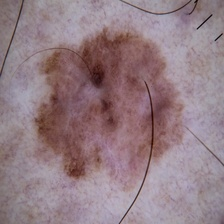
\includegraphics[width=\textwidth]{ej_ISIC_0024333.jpg}\\[2pt]
  {\scriptsize ISIC\_0024333\\ \emph{gt}: melanoma\\ Swin: melanoma}
\end{minipage}\hfill
\begin{minipage}[c]{0.72\textwidth}
\itshape ``\dots variegated color palette (brown, black, gray, red)\dots\ irregular borders\dots\ a
hallmark of melanoma. The color variegation is a key feature\dots\ irregular borders\dots\ a hallmark of
melanoma. The color variegation\dots'' \upshape \\[2pt]
Diagnóstico correcto y rasgos pertinentes, pero el texto \emph{repite} las mismas frases (degeneración
por repetición). Buen contenido diagnóstico, con una limitación de fluidez a vigilar.
\end{minipage}
}}
\caption{Un reporte diagnósticamente correcto puede aún presentar artefactos de generación, una
limitación de calidad textual distinta de la fidelidad diagnóstica.}
\label{fig:ej_rep}
\end{figure}

% ============================================================
\section{Costo computacional}
\label{sec:costo}
% ============================================================
Un eje central de la tesina es el \emph{costo}: hallar una estructura que funcione en hardware modesto y
se acerque a los modelos grandes, en lugar de asumir que un supermodelo lo resuelve todo. Se reportan dos
dimensiones de costo: el \textbf{costo temporal} —el \emph{tiempo de procesamiento de un ítem}, es decir
clasificar una imagen o generar un reporte, con \emph{batch}=1— y el \textbf{costo espacial} —la memoria
de GPU (VRAM) necesaria para cargar y ejecutar el modelo, que determina qué hardware puede alojarlo—. El
Cuadro~\ref{tab:costo} los resume (clasificadores medidos en una RTX 4070; VLMs, en A30 a partir de los
registros de las corridas: el tiempo por reporte se obtiene dividiendo el \emph{wall-clock} de cada job
por la cantidad de reportes generados).

\begin{table}[H]
  \centering
  \caption{Costo de inferencia. Tiempo por ítem de clasificadores: por imagen (\emph{batch}=1); de VLMs:
  por reporte generado. VRAM (costo espacial): estimación por pesos en clasificadores, pico observado en
  VLMs. Mejor (menor tiempo) por grupo en negrita.}
  \label{tab:costo}
  \small
  \begin{tabular}{llccc}
    \toprule
    \textbf{Modelo} & \textbf{Tipo} & \textbf{Params} & \textbf{VRAM (espacial)} & \textbf{Tiempo/ítem} \\
    \midrule
    ConvNeXt-Tiny        & Clasificador     & 28.6\,M & $\sim$0.6\,GB & \textbf{3.9\,ms} \\
    Swin-Tiny            & Clasificador     & 28.3\,M & $\sim$0.6\,GB & 8.7\,ms \\
    DenseNet121          & Clasificador     & 8.0\,M  & $\sim$0.5\,GB & 11.5\,ms \\
    DermLIP (ViT-B/16)   & VL-classifier    & 150\,M  & $\sim$2\,GB   & $\sim$15\,ms \\
    \midrule
    Mini-VLM (Phi-3.5-V) & VLM generativo   & 4.2\,B  & 10\,GB        & 24\,s \\
    SkinVL-MM            & VLM generativo   & 7\,B    & 14\,GB        & \textbf{$\sim$4\,s} \\
    LLaVA-Med v1.5       & VLM generativo   & 7\,B    & 14\,GB        & 66\,s \\
    \bottomrule
  \end{tabular}
\end{table}

\begin{figure}[H]
  \centering
  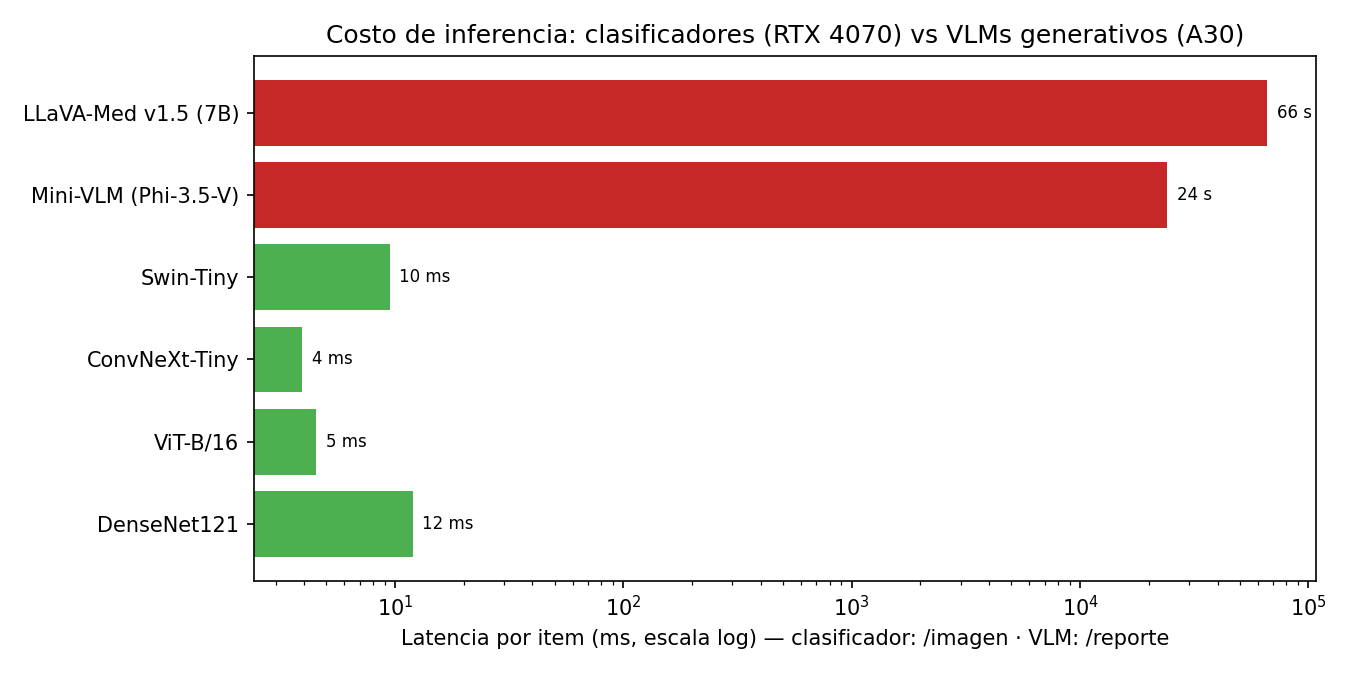
\includegraphics[width=0.92\textwidth]{P04_cost.png}
  \caption{Tiempo de procesamiento por ítem en escala logarítmica: clasificadores (verde, ms/imagen, RTX
  4070) vs VLMs generativos (rojo, s/reporte, A30). La brecha es de $\sim$3--4 órdenes de magnitud.}
  \label{fig:costo}
\end{figure}

\paragraph{Costo entre clasificadores.} Los tres clasificadores supervisados diagnostican en $4$--$12$\,ms
con menos de $1$\,GB de VRAM; DermLIP, siendo mayor ($150$\,M, $\sim$2\,GB), sigue en el rango de los
milisegundos. Las diferencias entre ellos son de \emph{fracciones de milisegundo} y de pocos cientos de
MB: a efectos prácticos, cualquiera de los cuatro corre holgadamente en una GPU de consumo e incluso en
CPU. La elección del clasificador se decide por exactitud, no por costo.

\paragraph{Costo entre generadores.} Entre los VLMs generativos sí hay diferencias relevantes. Mini-VLM
($4.2$\,B, $10$\,GB) entra en una GPU de consumo de gama alta; LLaVA-Med y SkinVL ($7$\,B, $14$\,GB)
requieren una GPU de más memoria. En tiempo, Mini-VLM ($24$\,s) es $\sim$$2.7\times$ más rápido que
LLaVA-Med ($66$\,s); SkinVL, pese a compartir tamaño con LLaVA-Med, resulta el más rápido ($\sim$4\,s)
\emph{precisamente porque produce reportes muy cortos} —el mismo colapso de estilo que lastra su
fidelidad (Sección~\ref{sec:skinvl}) abarata su generación—. Un tiempo bajo no es aquí una virtud:
refleja que el modelo dice poco.

\paragraph{Dónde vive el costo en el ensamble.} Comparar directamente los milisegundos de un clasificador
con los segundos de un generador \emph{no es una comparación justa} —son tareas distintas: una asigna una
etiqueta, la otra redacta texto—. El valor de contrastarlos es \emph{ubicar el costo dentro del
\emph{pipeline}} de dos etapas. La brecha es de \textbf{tres a cuatro órdenes de magnitud} (Mini-VLM es $\sim$$6000\times$ y LLaVA-Med
$\sim$$17\,000\times$ más lentos por ítem que ConvNeXt), de modo que en el ensamble el paso de
clasificación es \emph{despreciable} y la generación domina la cuenta, tanto en tiempo como en memoria
(Figura~\ref{fig:costo}).
La lectura para la tesina es que \emph{la tarea determina el costo del hardware}: para la
detección/diagnóstico basta hardware modesto (un clasificador o DermLIP), y el costo alto aparece solo al
generar el reporte. Mini-VLM ($24$\,s, $10$\,GB) es el mejor candidato de ``hardware modesto'' para la
generación, ya que con \emph{grounding} alcanza la consistencia de los modelos más grandes.

\paragraph{Costo de las ejecuciones completas.} Las cifras anteriores son \emph{por ítem}. Conviene
distinguir dos costos globales de otra naturaleza: el de \textbf{entrenar} (una sola vez) y el de
\textbf{evaluar/generar} sobre todo el conjunto (Cuadro~\ref{tab:costo_total}). El entrenamiento de un
\emph{clasificador} es barato ($\sim$2--4\,h en una RTX 4080, $\sim$6--8\,GB de VRAM); el de un
\emph{VLM generativo} con LoRA es el más caro en tiempo —Mini-VLM $9.4$\,h y LLaVA-Med $7.0$\,h en una A30
(medido), con $\sim$10--14\,GB de VRAM y $\sim$32\,GB de RAM de host—. Del lado de la \emph{evaluación}, la
asimetría es enorme: clasificar las $1503$ imágenes de test cuesta \emph{segundos} de inferencia ($\approx
4$\,s con TTA; unos minutos si se cuenta la carga del modelo/datos y el cómputo de todas las métricas),
mientras que \emph{generar} los reportes es el verdadero cuello de botella. Producir los reportes de un VLM
sobre el test completo tomó, según el modelo y la cantidad de condiciones de \emph{grounding} incluidas,
entre $\sim$$7.5$ y $20$\,h (Mini-VLM) y entre $13.6$ y \textbf{más de $37$\,h} (LLaVA-Med) —el extremo
superior corresponde a generar todas las condiciones, consumiendo $\sim$26--31\,GB de
RAM de host (Cuadro~\ref{tab:costo_total})—: los modelos de $7$\,B \emph{superan el límite de $48$\,h del
clúster en una sola corrida}, de modo que completar las $1503$ imágenes en todas las condiciones exigió
\emph{encadenar varias corridas} apoyándose en el \emph{resume} defensivo (que saltea los reportes ya
escritos). Es decir, tanto en entrenamiento como en evaluación, el costo global del pipeline se concentra
—de forma abrumadora— en el componente generativo, no en el de detección.

\begin{table}[H]
  \centering
  \caption{Costo global de entrenamiento (una vez) y de evaluación/generación sobre el test completo, con
  tiempos \emph{medidos} de los \emph{jobs} reales (clasificadores en RTX 4080; VLMs en A30, entrenamiento
  de la segunda etapa y generación sobre HAM). ``Generación completa'' = todas las condiciones de
  \emph{grounding} (baseline, DermLIP, Swin, oracle) sobre las $1503$ imágenes; la memoria de los VLMs es
  RAM de host (\emph{MaxRSS}), la VRAM ronda $10$--$14$\,GB.}
  \label{tab:costo_total}
  \small
  \begin{tabular}{lccc}
    \toprule
    \textbf{Proceso} & \textbf{Tiempo} & \textbf{Memoria} & \textbf{Tipo de costo} \\
    \midrule
    Entrenar un clasificador (Swin/ConvNeXt) & $\sim$2--4\,h & $\sim$6--8\,GB VRAM & una vez \\
    Entrenar VLM LoRA — Mini-VLM (etapa 2)   & $9.4$\,h & $\sim$10\,GB VRAM & una vez \\
    Entrenar VLM LoRA — LLaVA-Med (etapa 2)  & $7.0$\,h & $\sim$14\,GB VRAM & una vez \\
    Clasificar el test completo ($1503$)     & $\approx$4\,s (inferencia) & $<$1\,GB VRAM & por evaluación \\
    Generar reportes — Mini-VLM (test completo) & $\sim$7.5--20\,h & $\sim$26\,GB RAM & por evaluación \\
    Generar reportes — LLaVA-Med (test completo) & $13.6$--${>}37$\,h$^{\dagger}$ & $\sim$31\,GB RAM & por evaluación \\
    \bottomrule
  \end{tabular}
  \\[2pt]
  {\footnotesize $^{\dagger}$Superó el límite de $48$\,h del clúster en una sola corrida: completar las
  $1503$ imágenes en todas las condiciones requirió varias corridas encadenadas con \emph{resume}.}
\end{table}

% ============================================================
\section{Discusión y conclusiones}
\label{sec:conclusion}
% ============================================================
Los objetivos específicos de la experimentación son: (a) diseñar y evaluar modelos de detección —de \emph{deep
learning} y VLM— para identificar lesiones (en particular melanoma); (b) entrenar un VLM capaz de
integrar visión y texto para producir diagnósticos preliminares y reportes; y (c) evaluar el desempeño
en distintos escenarios (precisión diagnóstica, coherencia textual, utilidad). La evidencia recogida
permite responderlos de forma parcial:

\begin{enumerate}[leftmargin=1.6em]
  \item \textbf{Detección/clasificación (objetivo a).} Los clasificadores supervisados resuelven bien la
  tarea (Swin-Tiny F1 = 0.882). Los VLMs médicos \emph{generales} no son competitivos: su sensibilidad
  macro está al nivel del azar (Cuadro~\ref{tab:clasificacion}, Figura~\ref{fig:colapso}). Se mostró que
  no se debe al desbalance ni a la modalidad dermatoscópica (Sección~\ref{sec:rediag}), y que la
  literatura constata el mismo fenómeno de colapso al evaluar estos VLMs sobre HAM10000. En cambio, un
  VL model \emph{derm-especializado} (DermLIP) recupera la discriminación
  (Sección~\ref{sec:dermlip}). Es decir: para detectar lesiones, la especialización —no la mera
  capacidad ``visión--lenguaje''— es lo determinante. Para el problema clínicamente más crítico dentro de
  la detección —el melanoma, que el objetivo (a) nombra explícitamente—, la evaluación binaria
  melanoma-vs-resto (Sección~\ref{sec:melanoma}) muestra discriminación alta (AUC-ROC $0.93$--$0.95$) y,
  al optimizar el punto de operación en validación, baja la tasa de falsos negativos de $0.27$ (argmax) a
  $0.07$, con clasificadores \emph{Tiny} sobre GPU de consumo.
  \item \textbf{Generación de reportes (objetivo b).} Los VLMs generativos producen reportes ricos pero,
  por sí solos, no se comprometen con un diagnóstico (Sección~\ref{sec:reprazon}). El ensamble en
  cascada con \emph{grounding} (Sección~\ref{sec:porque_ensamble}) sí produce reportes que afirman un
  diagnóstico: con un clasificador fuerte, la \emph{diagnostic consistency} sube sustancialmente
  (Mini-VLM: $0.25 \rightarrow 0.81$, sobre las 1503 imágenes). Las ablaciones precisan \emph{de dónde} viene esa fidelidad: es el
  \textbf{diagnóstico del clasificador}, no la visión del generador, lo que la determina. En los tres
  generadores, quitarle la imagen al generador no baja la fidelidad —incluso la \emph{sube} en LLaVA-Med
  ($\Delta=-0.15$)—, mientras que inyectarle un diagnóstico equivocado la derrumba ($0.07$--$0.11$,
  Cuadro~\ref{tab:ablaciones}). Incluso un generador \emph{derm-especializado} (SkinVL,
  Sección~\ref{sec:skinvl}) confirma el patrón: sin \emph{grounding} colapsa, y con él acierta gracias a
  la etiqueta que recibe, no a lo que ``ve''. Consistente con esto, la fidelidad puede anclarse
  indistintamente con un clasificador entrenado o con \emph{recuperación} no paramétrica de casos
  similares (RAG sobre embeddings DermLIP, Sección~\ref{sec:rag}), que casi lo iguala y además enriquece
  el reporte —otra manifestación de que lo determinante es la representación especializada—. El
  \emph{grounding} simple, sin embargo, sigue comprometiéndose con un único diagnóstico aun cuando el
  clasificador tiene baja confianza. El \textbf{ensamble consciente de la incertidumbre}
  (Sección~\ref{sec:incertidumbre}) resuelve esto: afirma cuando dos clasificadores baratos coinciden,
  da un diferencial cuando no, y deriva a un especialista en el $4\%$ de máxima ambigüedad. Validado
  \emph{end-to-end} sobre los reportes generados, sube la \emph{diagnostic consistency} de $0.82$
  (\emph{grounding} simple) a $\mathbf{0.94}$ sobre los casos no derivados (Cuadro~\ref{tab:incertidumbre_e2e}),
  y en el subconjunto donde el clasificador duda, el reporte diferencial menciona el diagnóstico correcto el
  $90\%$ de las veces frente al $39\%$ del \emph{grounding} forzado.
  \item \textbf{Evaluación en distintos escenarios (objetivo c).} Se evaluó precisión diagnóstica
  (clasificación y Nivel 2 de reportes), coherencia/calidad textual (Nivel 1 y ejemplos cualitativos) y
  el comportamiento entre dominios de imagen (dermatoscopía vs clínica). Surgió además un aporte
  metodológico: al evaluar reportes provenientes de datos tipo \emph{Chain-of-Thought} es necesario
  separar el \emph{reporte} del \emph{razonamiento}, pues evaluar el texto completo sobreestima la
  fidelidad.
\end{enumerate}

\noindent\textbf{Síntesis (parcial).} La evidencia hasta el momento sugiere que, para \emph{diagnosticar},
conviene un modelo especializado (supervisado o VL derm-específico) —incluyendo el caso clínicamente más
crítico, melanoma, donde ese mismo tipo de modelo alcanza AUC $0.93$--$0.95$ con una tasa de falsos
negativos que baja a $0.07$ al fijar el punto de operación—, y que, para \emph{reportar}, un VLM
generativo \emph{anclado} a un clasificador produce reportes más fieles que un VLM por sí solo, mejorando
aún más cuando el anclaje es \emph{consciente de la incertidumbre} (afirmar, dar un diferencial o derivar
según la confianza), que sube la fidelidad de $0.82$ a $0.94$ sobre los casos no derivados. Ningún
VLM general resolvió, por sí mismo, ambas tareas; un ensamble de modelos especializados —chicos, sobre
GPU de consumo, en línea con el eje de \textbf{hardware accesible} planteado desde la
Introducción— se perfila como una vía efectiva para el objetivo de la experimentación. Estas conclusiones
valen dentro del alcance evaluado —dermatoscopía de HAM10000, medida con métricas automáticas—, cuyos
límites se detallan en las dos secciones siguientes.

\subsection{Amenazas a la validez}
\label{sec:amenazas}
Las cautelas metodológicas están señaladas a lo largo del documento; se las consolida acá según el tipo de
validez que afectan.
\begin{itemize}[leftmargin=1.6em]
  \item \textbf{Validez interna (protocolos mixtos).} Conviven mediciones \emph{single-view} y con
  \emph{test-time augmentation} (TTA) según el experimento: el \emph{headline} de clasificación usa TTA
  (Cuadro~\ref{tab:clasificacion}), mientras que calibración, robustez y el checkpoint de anclaje del
  pipeline de generación se miden single-view (notas de los Cuadros~\ref{tab:calib} y \ref{tab:ensamble}).
  Cada cuadro declara su protocolo, pero la comparación directa de valores absolutos entre cuadros exige
  tenerlo en cuenta. Asimismo, algunos números puntuales (razonamiento vs.\ reporte, ajuste de
  \emph{prompt}) provienen de condiciones controladas y no son directamente comparables con los cuadros.
  \item \textbf{Validez externa (un dataset principal).} El grueso de la evaluación es sobre HAM10000
  (dermatoscopía); HIBA se usa solo como conjunto OOD, y la caída de $27$--$40$ puntos allí
  (Sección~\ref{sec:robustez}) acota la generalización a otras poblaciones y equipos de adquisición. Las
  comparaciones con el estado del arte son \textbf{orientativas}: los protocolos y datasets difieren
  (Cuadros~\ref{tab:sota_clasif}, \ref{tab:sota_melanoma}, \ref{tab:sota_gen}). El mapeo de etiquetas
  HIBA$\to$HAM introduce además algo de ruido de anotación (Sección~\ref{sec:robustez}).
  \item \textbf{Validez de constructo (métricas como \emph{proxies}).} La fidelidad se mide con
  \emph{diagnostic consistency} y \emph{clinical entity recall} (Nivel 2), que aproximan pero no equivalen
  al juicio de un especialista, que no interviene en ninguna de las evaluaciones reportadas. Las métricas
  léxicas de Nivel 1 (BLEU/ROUGE) penalizan el estilo más que la calidad clínica
  (Secciones~\ref{sec:skincot} y discusión del Cuadro~\ref{tab:sota_gen}), por lo que se las interpreta con
  cautela.
\end{itemize}

\subsection{Limitaciones}
\label{sec:limitaciones}
La experimentación se da por cerrada con los resultados reportados hasta acá. Lo que sigue delimita
\emph{hasta dónde} llegan esas conclusiones.
\begin{itemize}[leftmargin=1.6em]
  \item \textbf{Escala de la evaluación de reportes.} La comparación central del ensamble
  (Cuadro~\ref{tab:ensamble}) se evaluó sobre el \emph{test split completo} (1503 imágenes) para los tres
  generadores. Las ablaciones más finas (imagen-vs-dx, dx-erróneo, Cuadro~\ref{tab:ablaciones}) se hicieron
  sobre un subconjunto de 400 imágenes por su costo de generación; los valores centrales sobre 400 y sobre
  1503 coinciden estrechamente (p.ej.\ Mini-VLM con Swin $0.830$ vs $0.812$), lo que respalda la
  representatividad del subconjunto.
  \item \textbf{Costo experimental.} Cada prueba que involucra VLMs o generación de reportes requiere
  enviar trabajos al clúster Mendieta (por la memoria de GPU necesaria), con tiempos de espera en cola
  de aproximadamente 4 a 6 días en muchos casos. Esto limitó fuertemente la cantidad de iteraciones posibles
  y condicionó el diseño de los experimentos (p.\,ej.\ usar subconjuntos, paralelizar trabajos).
  \item \textbf{Ausencia de reportes redactados por especialistas.} Ninguno de los conjuntos usados
  contiene reportes \emph{escritos} por un dermatólogo: la referencia más cercana es SkinCoT, cuyas
  narrativas las genera un pipeline de modelos de lenguaje y las \emph{certifican} dermatólogos
  (Figura~\ref{fig:human_vs_gen}). Esa comparación cualitativa solo es posible sobre SkinCoT,
  el único conjunto con referencias humanas; sobre HAM10000 (dermatoscopía) no hay reportes de referencia,
  de modo que allí la fidelidad se mide contra la etiqueta diagnóstica (Nivel 2), no contra un texto
  humano. No existe públicamente un corpus de reportes dermatoscópicos redactados por especialistas, de
  modo que la comparación lado a lado no puede extenderse más allá de SkinCoT.
  \item \textbf{Generalización fuera de distribución.} La caída de $27$--$40$ puntos de exactitud sobre
  HIBA (Sección~\ref{sec:robustez}) muestra que los clasificadores no transfieren bien a otra población
  (fototipos III--VI). Eso acota el alcance de todo lo reportado acá: como es el clasificador el que ancla
  la fidelidad del ensamble, la mejora de $0.82$ a $0.94$ en \emph{diagnostic consistency} no debe leerse
  como transferible a una población distinta de la evaluada.
  \item \textbf{Anclajes no evaluados.} El ensamble de generación solo se probó con Swin y con DermLIP
  zero-shot/linear-probe como clasificador de anclaje. El SVM-RBF sobre \emph{embeddings} congelados de
  DermLIP (Sección~\ref{sec:dermlip}), que iguala o supera a Swin en Acc/F1, nunca se usó en ese rol, de
  modo que la relación entre exactitud del ancla y fidelidad del reporte se caracteriza sobre tres puntos
  ($0.38$, $0.80$, $1.00$) y no sobre un barrido.
  \item \textbf{Generadores no evaluados.} Los modelos de razonamiento clínico como
  Skin-R1 (\cite{liu2025skinr1}) no se probaron como generadores del ensamble. El otro candidato natural, un
  generador \emph{derm-especializado} (SkinVL~\cite{zeng2025mmskin}), sí se incorporó
  (Sección~\ref{sec:skinvl}) y su resultado —colapso sin \emph{grounding}, reportes muy breves con él—
  reforzó, en lugar de matizar, la conclusión de que la fidelidad proviene del clasificador; eso vuelve
  menos probable, aunque no descartable, que cambiar de generador altere el resultado central.
\end{itemize}

\printbibliography

\end{document}
